\documentclass[12pt,fullpage]{report}
\usepackage{fullpage}
\usepackage{graphicx}
\usepackage{times}
\usepackage{mdframed}
% \usepackage{authblk}
\usepackage{float}
\usepackage{cite}
% \usepackage{makeidx}
\usepackage{hyperref}
\usepackage{glossaries}
\usepackage[toc,page]{appendix}

\usepackage{listings}
\lstset{
   breaklines=true,
   basicstyle=\ttfamily
}
\linespread{1.1}

\setcounter{secnumdepth}{6}

% \makeindex
\makeglossaries

\begin{document}


%----------------------------------------------------------------------------------------
%       TITLE PAGE
%----------------------------------------------------------------------------------------
\newcommand*{\titleGM}{\begingroup % Create the command for including the title page in the document
\hbox{ % Horizontal box
\hspace*{0.5cm}

\includegraphics[scale=1.7]{Images/MGRAST_logo-green.png}%\hspace*{0.2\textwidth} % Whitespace to the left of the title page
\hspace*{0.02\textwidth} % Whitespace between the vertical line and title page text
\rule{1pt}{\textheight} % Vertical line
\hspace*{0.04\textwidth} % Whitespace between the vertical line and title page text
\parbox[b]{0.8\textwidth}{ % Paragraph box which restricts text to less than the width of the page
{\noindent\Huge\bfseries MG-RAST Manual}\\[0.8\baselineskip] 
{\noindent\Huge\bfseries for version 3.3.6,}\\[0.8\baselineskip] % Title
{\noindent\Huge\bfseries revision 10}\\[2\baselineskip] % Title
{\large \textit{November 15, 2014}}\\[4\baselineskip] % Tagline or further description
{\textbf{Andreas Wilke\textsuperscript{1,2},}}\\    % author name
{\textbf{Elizabeth M. Glass\textsuperscript{1,2},}}\\    % author name
{\textbf{Jared Bischof\textsuperscript{2,1},}}\\    % author name
{\textbf{Daniel Braithwaite\textsuperscript{1,2},}}\\    % author name
{\textbf{Mark D'Souza\textsuperscript{2,1},}}\\    % author name
{\textbf{Wolfgang Gerlach\textsuperscript{2,1},}}\\    % author name
{\textbf{Travis Harrison\textsuperscript{2,1},}}\\    % author name
{\textbf{Kevin Keegan\textsuperscript{1,2},}}\\    % author name
{\textbf{Hunter Matthews\textsuperscript{1,2},}}\\    % author name
{\textbf{Tobias Paczian\textsuperscript{2,1},}}\\    % author name
{\textbf{Wei Tang\textsuperscript{1,2},}}\\    % author name
{\textbf{William L. Trimble\textsuperscript{2,1},}}\\    % author name
{\textbf{Narayan Desai\textsuperscript{1,2} and}}\\    % author name
{\textbf{Folker Meyer\textsuperscript{1,2}}}\\[3\baselineskip]    % author name
{\noindent \textsuperscript{1}Argonne National Laboratory}\\   % affiliation
{\noindent \textsuperscript{2}University of Chicago}\\[\baselineskip] % affiliation
}
}
\endgroup}


\titleGM % This command includes the title page
\thispagestyle{empty}

%%%%%%%%%%%%%%%%%%%%%%%%%%%%%%%%%%%%%%%%%%%%%%%
%  begin old title page  %%%%%%%%%%%%%%%%%%%%%%%%%%%%%%%%%%%
%%%%%%%%%%%%%%%%%%%%%%%%%%%%%%%%%%%%%%%%%%%%%%%
% \usepackage{authblk}
% \author[1,2]{Andreas Wilke}
% \author[1,2]{Elizabeth M. Glass}
% \author[2,1]{Jared Bischof}
% \author[1,2]{Daniel Braithwaite}
% \author[2,1]{Mark D'Souza}
% \author[2,1]{Wolfgang Gerlach}
% \author[2,1]{Travis Harrison}
% \author[1,2]{Kevin Keegan}
% \author[1,2]{Hunter Matthews}
% \author[2,1]{Tobias Paczian}
% \author[1,2]{Wei Tang}
% \author[2.1]{William L. Trimble}
% \author[1,2]{Narayan Desai}
% \author[1,2]{Folker Meyer}
% \affil[1]{Argonne National Laboratory}
% \affil[2]{University of Chicago}
% \date{April 11, 2014}
% \title{
% \emph{\textbf{MG-RAST Manual\\
% for version 3.3.6,\\ revision 7}}
% }
% \maketitle
%%%%%%%%%%%%%%%%%%%%%%%%%%%%%%%%%%%%%%%%%%%%%%%
%  end old title page  %%%%%%%%%%%%%%%%%%%%%%%%%%%%%%%%%%%%
%%%%%%%%%%%%%%%%%%%%%%%%%%%%%%%%%%%%%%%%%%%%%%%


%\bibstyle{apsrev}
% \section{Review}

\pagenumbering{roman}
\tableofcontents

%\begin{abstract}
%The democratized world of sequencing is leading to numerous data analysis challenges; MG-RAST solves them for amplicon data sets, shotgun metagenomes, and metatranscriptomes. The changes from version 2 to version 3 include the addition of a dedicated gene calling stage using FragGenescan, clustering of predicted proteins at 90\% identity, and the use of BLAT for the computation of similarities. Together with changes in the underlying software infrastructure, this has enabled the dramatic scaling up of pipeline throughput while remaining on a limited hardware budget. The web based service allows upload, fully automated analysis and visualization of results. As a result of the plummeting cost of sequencing and the readily available analytical power of MG-RAST, over 78,000 metagenomic datasets have been analyzed, with over 12,000 of them publicly available in MG-RAST.
%Keywords: automated analysis of metagenomes, metatranscriptomes and amplicon data, public archive for data and analysis results, metadata enabled data discovery, scalable analysis pipeline
%\end{abstract}

% %%%%%%%%%%%%%%%%%%%%%%%%%%%%%%%%%%%%%%%%%%%%%%%%%%%%%%%%%%%%%%%%%%%%%%
% %%%%%%%%%%%%%%%%%%%%%%%%%%%%%%%%%%%%%%%%%%%%%%%%%%%%%%%%%%%%%%%%%%%%%%
% %%%%%%%%%%%%%%%%%%%%%%%%%%%%%%%%%%%%%%%%%%%%%%%%%%%%%%%%%%%%%%%%%%%%%%
% %%%%%%%%%%%%%%%%%%%%%%%%%%%%%%%%%%%%%%%%%%%%%%%%%%%%%%%%%%%%%%%%%%%%%%
\newcommand{\dictentry}[2]{%
  \newglossaryentry{#1}{name=#1,description={#2}}%
  \glslink{#1}{}%
}
\dictentry{DNA}{Deoxyribonucleic acid}
\dictentry{RNA}{Ribonucleic acid}
\dictentry{ADR}{Artificial duplicate read}
\dictentry{JSON}{JavaScript Object Notation}
\dictentry{EC2}{ Amazon Elastic Compute Cloud}
\dictentry{rRNA}{ribosomal ribonucleic acid}
\dictentry{16s}{16S ribosomal RNA (or 16S rRNA) is a component of the 30S small subunit of prokaryotic ribosomes}
\dictentry{SEED}{The SEED effort led by Ross Overbeek is a systematic annotation effort for prokaryotic genomes using Subsystems}
\dictentry{Subsystem}{A subsystem is a set of functional roles that an annotator has decided should be thought of as related. Frequently, subsystems represent the collection of functional roles that make up a metabolic pathway, a complex (e.g., the ribosome), or a class of proteins (e.g., two-component signal-transduction proteins within Staphylococcus aureus). Construction of a large set of curated populated subsystems is at the center of the SEED annotation efforts}
\dictentry{MD5}{The MD5 message-digest algorithm is a widely used cryptographic hash function that produces a 128-bit (16-byte) hash value. Specified in RFC 1321, MD5 has been utilized in a wide variety of security applications, and is also commonly used to check data integrity}
% %%%%%%%%%%%%%%%%%%%%%%%%%%%%%%%%%%%%%%%%%%%%%%%%%%%%%%%%%%%%%%%%%%%%%%
% %%%%%%%%%%%%%%%%%%%%%%%%%%%%%%%%%%%%%%%%%%%%%%%%%%%%%%%%%%%%%%%%%%%%%%
% %%%%%%%%%%%%%%%%%%%%%%%%%%%%%%%%%%%%%%%%%%%%%%%%%%%%%%%%%%%%%%%%%%%%%% 
% %%%%%%%%%%%%%%%%%%%%%%%%%%%%%%%%%%%%%%%%%%%%%%%%%%%%%%%%%%%%%%%%%%%%%%
\chapter{Introduction}
\setcounter{page}{1}
\pagenumbering{arabic}
% %%%%%%%%%%%%%%%%%%%%%%%%%%%%%%%%%%%%%%%%%%%%%%%%%%%%%%%%%%%%%%%%%%%%%%
% %%%%%%%%%%%%%%%%%%%%%%%%%%%%%%%%%%%%%%%%%%%%%%%%%%%%%%%%%%%%%%%%%%%%%% 
% %%%%%%%%%%%%%%%%%%%%%%%%%%%%%%%%%%%%%%%%%%%%%%%%%%%%%%%%%%%%%%%%%%%%%%
\section{Motivation}

The National Human Genome Research Institute (NHGRI), a division of the National Institutes of Health, publishes information (see Figure \ref{fig:cost_per_megabase}) describing the development of computing costs and DNA sequencing costs over time \cite{NHGRI_COST}. The dramatic gap between the shrinking costs of sequencing and the more or less stable costs of computing is a major challenge for biomedical researchers trying to use next-generation DNA sequencing platforms to obtain information on microbial communities. Wilkening \textit{et al.} \cite{MGCLOUD} provide a real currency cost for the analysis of 100 gigabasepairs of DNA sequence data using BLASTX on Amazon's \gls{EC2} service: \$300,000.\footnote{This includes only the computation cost, no data transfer cost, and was computed using 2009 prices.} A more recent study by University of Maryland researchers \cite{CLOVR} estimates the computation for a terabase of DNA shotgun data using their CLOVR metagenome analysis pipeline at over \$5 million per terabase.

\begin{figure*}
\begin{center}
 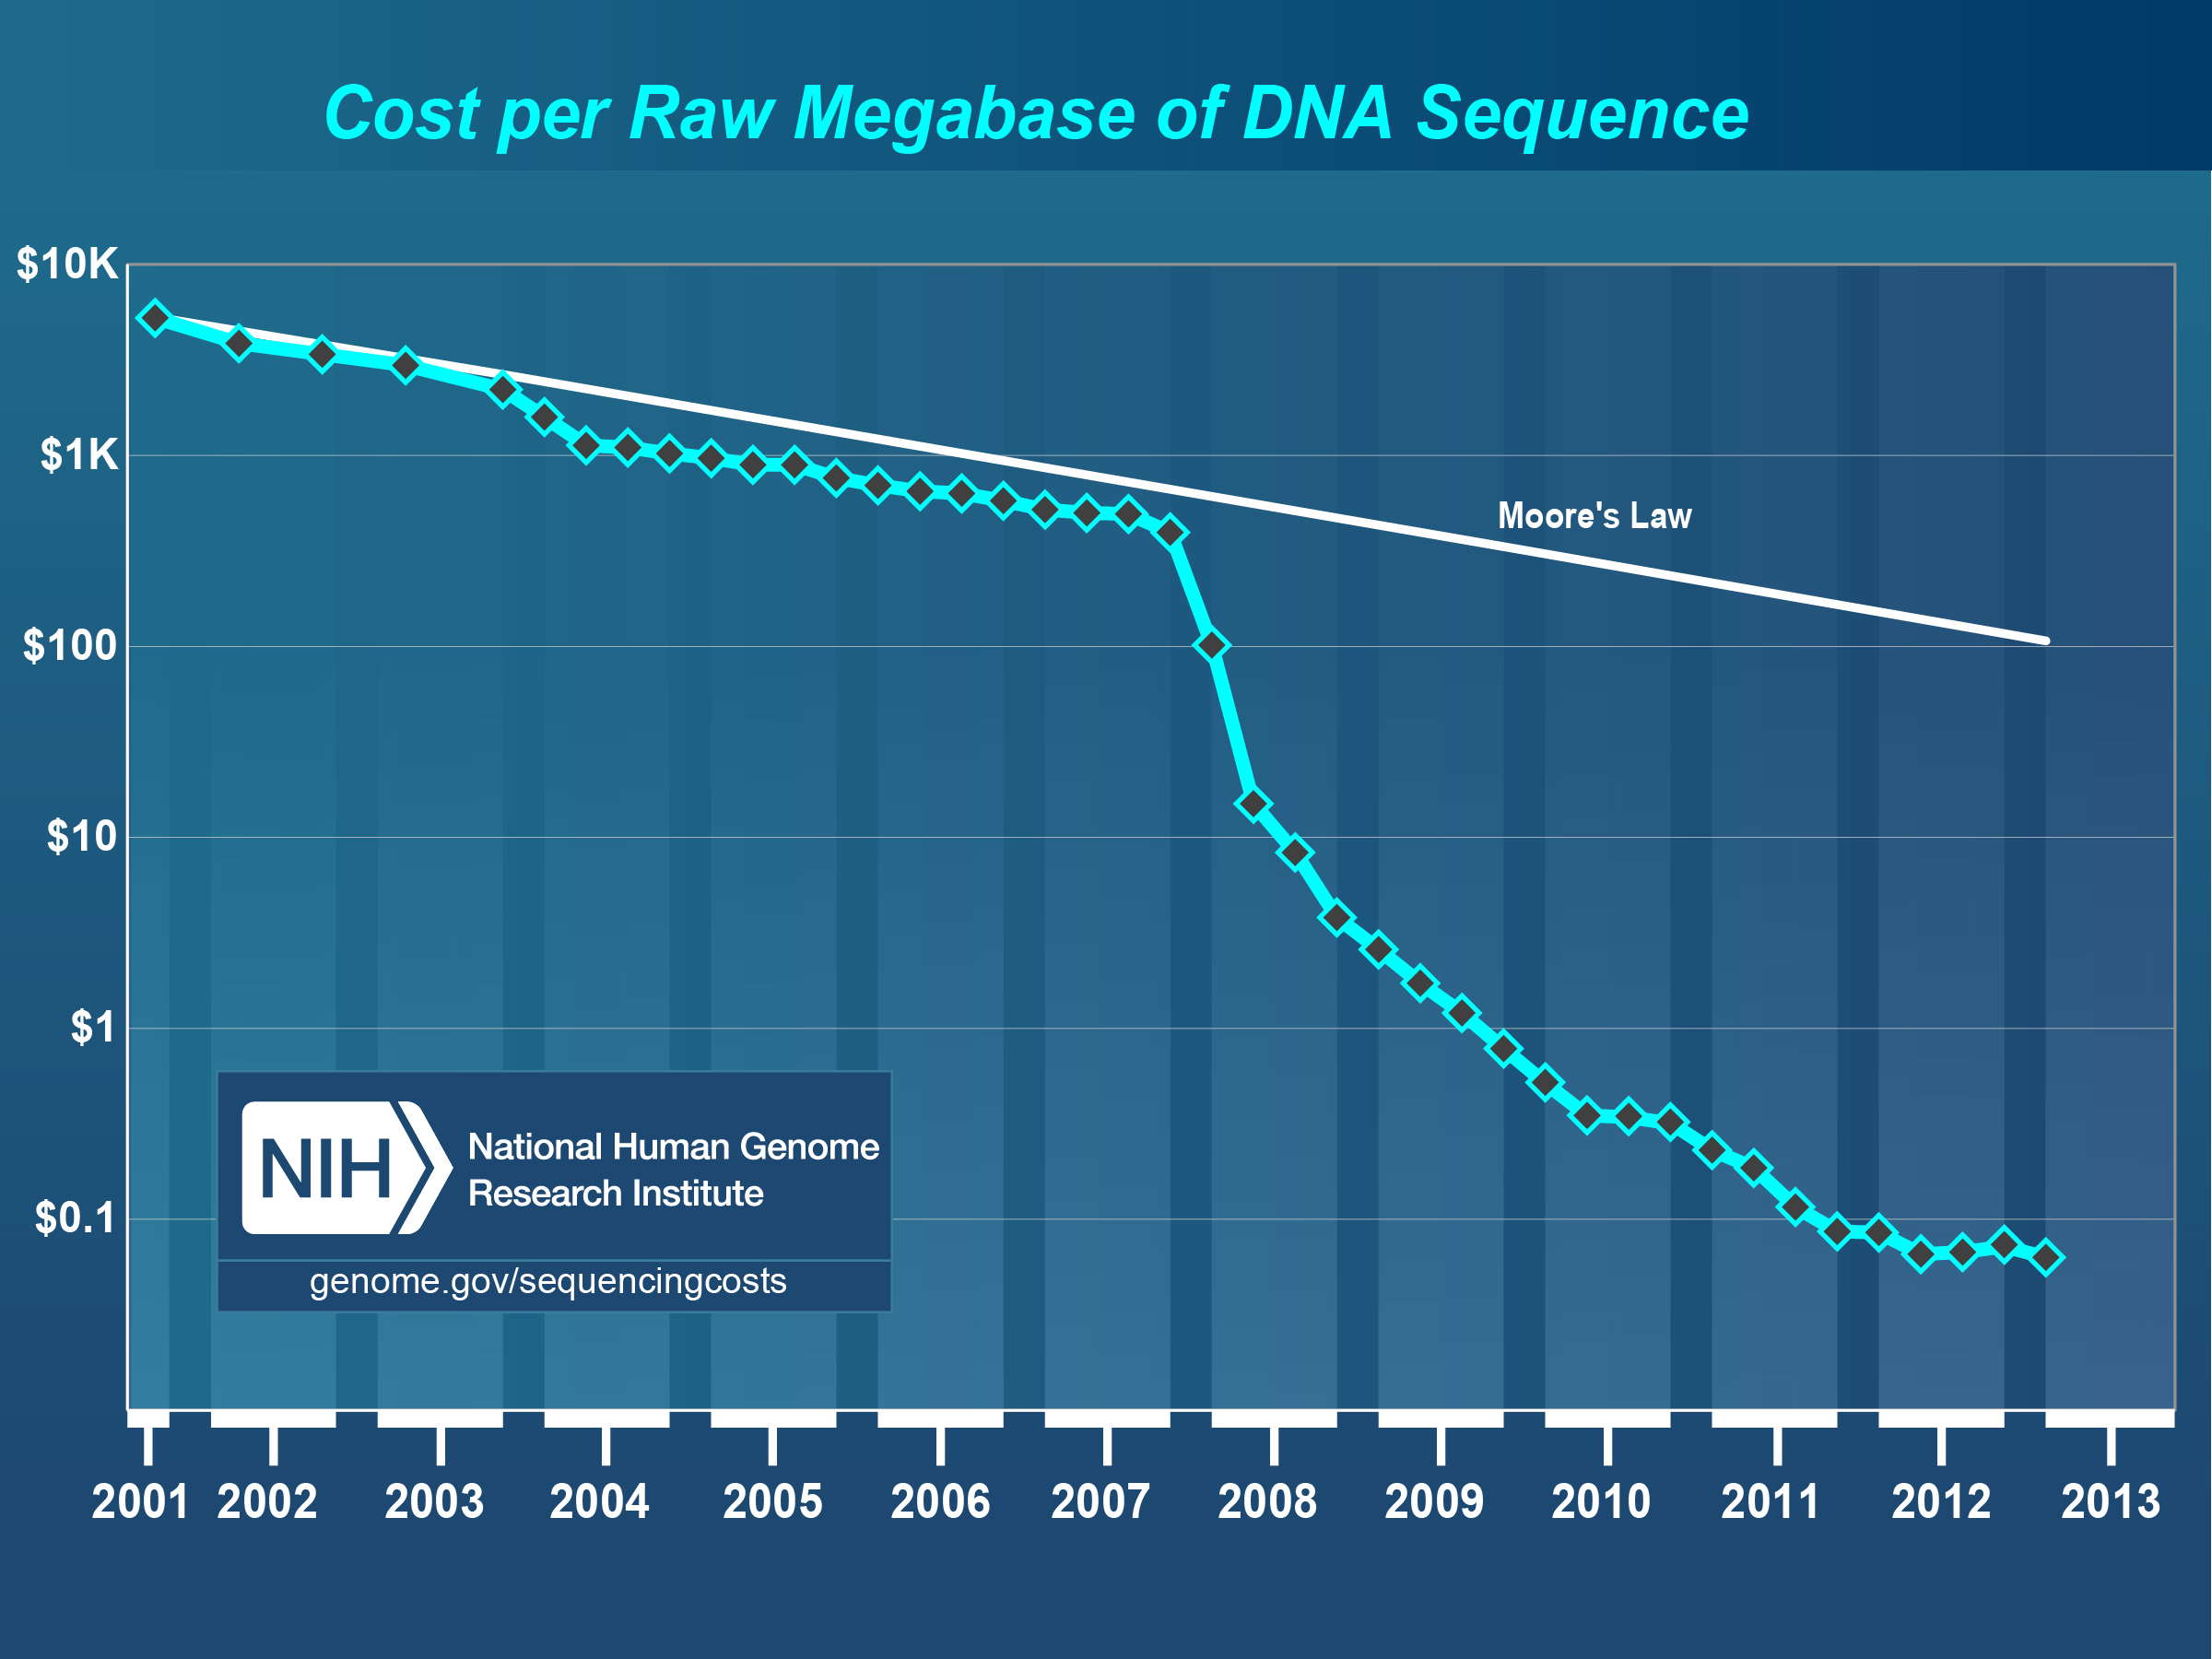
\includegraphics[width=4in]{Images/cost_per_megabase.png}
\end{center}
\label{fig:cost_per_megabase}
\caption{Chart showing shrinking cost for DNA sequencing. This comparison with Moore's law roughly describing the development of computing costs highlights the growing gap between sequence data and the available analysis resources. Source: NHGRI \cite{NHGRI_COST}
}
\end{figure*}

Nevertheless, the growth in data enabled by next-generation sequencing platforms also provides an exciting opportunity for studying microbial communities: ~99\% of the microbes in which have not yet been cultured \cite{MGREVIEW}. Cultivation-free methods (often summarized as metagenomics) offer novel insights into the biology of the vast majority of life on Earth \cite{THOMASREVIEW}.

Three types of metagenomics experiments are commonly used:

\begin{enumerate}

\item Environmental clone libraries (functional metagenomics):
use of Sanger sequencing (frequently) instead of more cost-efficient next-generation sequencing

\item Amplicon studies (single gene studies, \gls{16s} rDNA):
next-generation sequencing of PCR amplified ribosomal genes providing a single reference gene--based view of microbial community ecology

\item Shotgun metagenomics: 
use of next-generation technology applied directly to environmental samples
\end{enumerate}

\noindent
Each of these methods has strengths and weaknesses (see \cite{THOMASREVIEW}), as do the various sequencing technologies (see \cite{LOMAN}).

To support user-driven analysis of all types of metagenomic data, we have provided MG-RAST \cite{MG-RAST} to enable researchers to study the function and composition of microbial communities.
The MG-RAST portal offers automated quality control, annotation, comparative analysis, and archiving services.
At the time of writing (\date{\today}) MG-RAST has completed the analysis of over 45 terabasepairs of DNA data in over 115,000 datasets contributed by thousands of researchers worldwide.

The MG-RAST system provides answers to the following scientific questions:
\begin{itemize}
\item Who is out there?
Identifying the composition of a microbial community either by using amplicon data for single genes or by deriving community composition from shotgun metagenomic data using sequence similarities.

\item What are they doing?
Using shotgun data (or metatranscriptomic data) to derive the functional complement of a microbial community using similarity searches against a number of databases.

\item Who is doing what?
Based on sequence similarity searches, identifying the organisms encoding specific functions.
\end{itemize}

The system supports the analysis of the prokaryotic content of samples, analysis of viruses and eukaryotic sequences is not currently supported.

MG-RAST users can upload raw sequence data in fastq, fasta and sff format; the sequences will be normalized (quality controlled) and processed and summaries automatically generated. The server provides several methods to access the different data types, including phylogenetic and metabolic reconstructions, and the ability to compare the metabolism and annotations of one or more metagenomes, individually or in groups. Access to the data is password protected unless the owner has made it public, and all data generated by the automated pipeline is available for download in variety of common formats.
% %%%%%%%%%%%%%%%%%%%%%%%%%%%%%%%%%%%%%%%%%%%%%%%%%%%%%%%%%%%%%%%%%%%%%%
% %%%%%%%%%%%%%%%%%%%%%%%%%%%%%%%%%%%%%%%%%%%%%%%%%%%%%%%%%%%%%%%%%%%%%% 
% %%%%%%%%%%%%%%%%%%%%%%%%%%%%%%%%%%%%%%%%%%%%%%%%%%%%%%%%%%%%%%%%%%%%%% 
\section{Brief description}
\label{section:brief-description}
The MG-RAST pipeline performs quality control, protein prediction, clustering and similarity-based annotation on nucleic acid sequence datasets using a number of bioinformatics tools (see Section \ref{section:bioinformatics-codes}.  MG-RAST was built to analyze large shotgun metagenomic data sets ranging in size from megabases to terabases.  We also support amplicon (16s, 18s, ITS, �) sequence datasets and metatranscriptome (RNA-seq) sequence datasets.   The current MG-RAST pipeline is not capable of predicting coding regions from eukaryotes and thus will be of limited use for eukaryotic shotgun metagenomes and/or the eukaryotic subsets of shotgun metagenomes.

Data on MG-RAST is private to the submitting user unless shared with other users or made public by the user. We strongly encourage the eventual release of data and require metadata (``data describing data'') for data sharing or publication. Data submitted with metadata will be given priority for the computational queue.

You need to provide (raw or assembled) nucleotide sequence data and sample descriptions (``metadata''). The system accepts sequence data in FASTA, FASTQ and SFF format and metadata in the form or GSC (\begin{small}\url{http://gensc.org/}\end{small}) standard compliant checklists (see Yilmaz et al, Nature Biotech, 2011).   Uploads can be put in the system via either the web interface or a command line tool.   Data and metadata are validated after upload.
%http://www.nature.com/nbt/journal/v29/n5/full/nbt.1823.html?WT.ec_id=NBT-201105

You must choose quality control filtering options at the time you submit your job. MG-RAST provides several options for  quality control (QC) filtering for nucleotide sequence data, including  removal of artificial duplicate reads, quality-based read trimming, length-based read trimming, and screening for DNA of model organisms (or humans). These filters are applied before the data are submitted for annotation.

The MG-RAST pipeline assigns an accession number and puts the data in a queue for computation.  The similarity search step is computationally expensive. Small jobs can complete as fast as hours, while large jobs can spend a week waiting in line for computational resources.

MG-RAST performs a protein similarity search between predicted proteins and database proteins (for shotgun) and a nucleic-acid similarity search (for reads similar to 16S and 18S sequences). 
%These databases are searched.  refer  appendix

MG-RAST presents the annotations via the tools on the analysis page which prepare, compare, display, and export the results on the website. The download page offers the input data, data at intermediate stages of filtering, the similarity search output, and summary tables of functions and organisms detected.

MG-RAST can compare thousands of data sets run through a consistent annotation pipeline.  We also provide a means to view annotations in multiple different namespaces (e.g. SEED functions, K.O. Terms, Cog Classes, EGGnoggs) via the M5Nr.
% cite m5nr

The publication ``Metagenomics-a guide from sampling to data analysis'' (PMID 22587947) in Microbial Informatics and Experimentation, 2012 is a good review of best practices for experiment design for further reading.
% %%%%%%%%%%%%%%%%%%%%%%%%%%%%%%%%%%%%%%%%%%%%%%%%%%%%%%%%%%%%%%%%%%%%%%
% %%%%%%%%%%%%%%%%%%%%%%%%%%%%%%%%%%%%%%%%%%%%%%%%%%%%%%%%%%%%%%%%%%%%%% 
% %%%%%%%%%%%%%%%%%%%%%%%%%%%%%%%%%%%%%%%%%%%%%%%%%%%%%%%%%%%%%%%%%%%%%% 
\section{URL}
\label{section:MG-RAST-URL}
\url{http://metagenomics.anl.gov/}
% %%%%%%%%%%%%%%%%%%%%%%%%%%%%%%%%%%%%%%%%%%%%%%%%%%%%%%%%%%%%%%%%%%%%%% 
% %%%%%%%%%%%%%%%%%%%%%%%%%%%%%%%%%%%%%%%%%%%%%%%%%%%%%%%%%%%%%%%%%%%%%% 
% %%%%%%%%%%%%%%%%%%%%%%%%%%%%%%%%%%%%%%%%%%%%%%%%%%%%%%%%%%%%%%%%%%%%%% 
\section{Citing MG-RAST}
\label{section:MG-RAST-citation}
If you use our service, please cite: \\
\noindent
The Metagenomics RAST server --- A public resource for the automatic phylogenetic and functional analysis of metagenomes \\
\noindent
F. Meyer, D. Paarmann, M. D'Souza, R. Olson , E. M. Glass, M. Kubal, T. Paczian, A. Rodriguez, R. Stevens, A. Wilke, J. Wilkening, and R. A. Edwards \\
\noindent
BMC Bioinformatics 2008, 9:386 \\
\noindent
\begin{small}\url{http://www.biomedcentral.com/1471-2105/ 9/386}\end{small}.
% %%%%%%%%%%%%%%%%%%%%%%%%%%%%%%%%%%%%%%%%%%%%%%%%%%%%%%%%%%%%%%%%%%%%%% 
% %%%%%%%%%%%%%%%%%%%%%%%%%%%%%%%%%%%%%%%%%%%%%%%%%%%%%%%%%%%%%%%%%%%%%% 
% %%%%%%%%%%%%%%%%%%%%%%%%%%%%%%%%%%%%%%%%%%%%%%%%%%%%%%%%%%%%%%%%%%%%%% 
\section{Version history}
% %%%%%%%%%%%%%%%%%%%%%%%%%%%%%%%%%%%%%%%%%%%%%%%%%%%%%%%%%%%%%%%%%%%%%%
% %%%%%%%%%%%%%%%%%%%%%%%%%%%%%%%%%%%%%%%%%%%%%%%%%%%%%%%%%%%%%%%%%%%%%% 
\subsection*{Version 1}
The original version of MG-RAST was developed in 2007 by Folker Meyer, Andreas Wilke, Daniel Paarman, Bob Olson, and Rob Edwards. It relied heavily on the \gls{SEED}\cite{SUBSYSTEMS} environment and allowed upload of preprocessed 454 and Sanger data.
% %%%%%%%%%%%%%%%%%%%%%%%%%%%%%%%%%%%%%%%%%%%%%%%%%%%%%%%%%%%%%%%%%%%%%%
% %%%%%%%%%%%%%%%%%%%%%%%%%%%%%%%%%%%%%%%%%%%%%%%%%%%%%%%%%%%%%%%%%%%%%% 
\subsection*{Version 2}
Version 2, released in 2008, had numerous improvements. It was optimized to handle full-sized 454 datasets and was the first version of MG-RAST that was not fully \gls{SEED} based.
Version 2.0 used BLASTX analysis for both gene prediction and functional classification\cite{MG-RAST}.
% %%%%%%%%%%%%%%%%%%%%%%%%%%%%%%%%%%%%%%%%%%%%%%%%%%%%%%%%%%%%%%%%%%%%%%
% %%%%%%%%%%%%%%%%%%%%%%%%%%%%%%%%%%%%%%%%%%%%%%%%%%%%%%%%%%%%%%%%%%%%%% 
\subsection*{Version 3}
While version 2 of MG-RAST was widely used, it was limited to datasets smaller than a few hundred megabases, and comparison of samples was limited to pairwise comparisons. Version 3 is not based on \gls{SEED} technology; instead, it uses the SEED subsystems as a preferred data source.
Starting with version 3, MG-RAST moved to github.
% %%%%%%%%%%%%%%%%%%%%%%%%%%%%%%%%%%%%%%%%%%%%%%%%%%%%%%%%%%%%%%%%%%%%%%
% %%%%%%%%%%%%%%%%%%%%%%%%%%%%%%%%%%%%%%%%%%%%%%%%%%%%%%%%%%%%%%%%%%%%%%
% %%%%%%%%%%%%%%%%%%%%%%%%%%%%%%%%%%%%%%%%%%%%%%%%%%%%%%%%%%%%%%%%%%%%%% 
\section{Comparison of versions 2 and 3}

In the 3.0 version, datasets of tens of gigabases can be annotated, and comparison of taxa or functions that differ between samples is now limited only by the available screen real estate. Figure \ref{fig:mgrastv2VSv3} shows a comparison of the analytical and computational approaches used in MG-RAST v2 and v3. The major changes are the inclusion of a dedicated gene-calling stage using FragGenescan \cite{FGS}, clustering of predicted proteins at 90\% identified by using uclust \cite{UCLUST}, and the use of BLAT \cite{BLAT} for the computation of similarities. Together with changes in the underlying infrastructure, this version has allowed dramatic scaling of the analysis with the limited hardware available.

Similar to version 2.0, the new version of MG-RAST does not pretend to know the correct parameters for the transfer of annotations. Instead, users are empowered to choose the best parameters for their datasets.

\begin{figure*}
\begin{center}
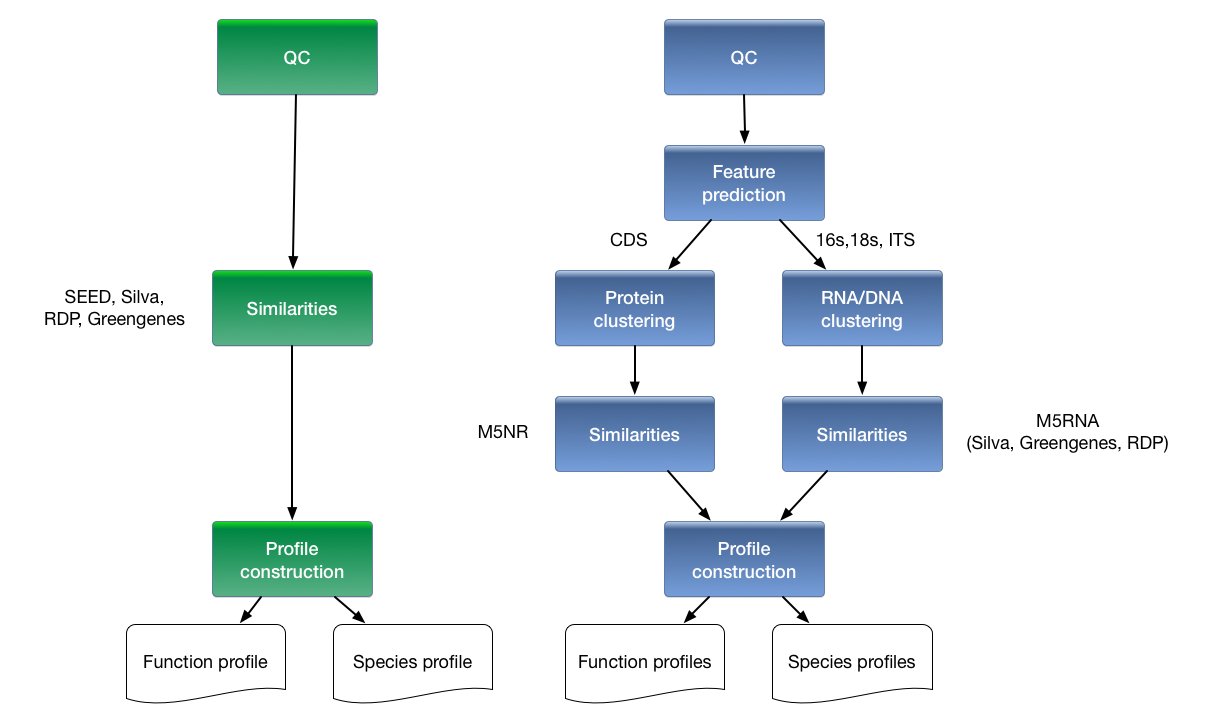
\includegraphics[width=6in]{Images/mgrastv2VSv3.png}
\end{center}
\caption{
Overview of processing pipeline in (left) MG-RAST v2 and (right) MG-RAST v3. In the old pipeline, metadata was rudimentary, compute steps were performed on individual reads on a 40-node cluster that was tightly coupled to the system, and similarities were computed by BLAST to yield abundance profiles that could then be compared on a per sample or per pair basis. In the new pipeline, rich metadata can be uploaded, normalization and feature prediction are performed, faster methods such as BLAT are used to compute similarities, and the resulting abundance profiles are fed into downstream pipelines on the cloud to perform community and metabolic reconstruction and to allow queries according to rich sample and functional metadata.
}
\label{fig:mgrastv2VSv3}
\end{figure*}

The new version of MG-RAST represents a rethinking of core processes and data products, as well as new user interface metaphors and a redesigned computational infrastructure. MG-RAST supports a variety of user-driven analyses, including comparisons of many samples, previously too computationally intensive to support for an open user community.

Scaling to the new workload required changes in two areas: the underlying infrastructure needed to be rethought, and the analysis pipeline needed to be adapted to address the properties of the newest sequencing technologies.
% %%%%%%%%%%%%%%%%%%%%%%%%%%%%%%%%%%%%%%%%%%%%%%%%%%%%%%%%%%%%%%%%%%%%%%
% %%%%%%%%%%%%%%%%%%%%%%%%%%%%%%%%%%%%%%%%%%%%%%%%%%%%%%%%%%%%%%%%%%%%%%
% %%%%%%%%%%%%%%%%%%%%%%%%%%%%%%%%%%%%%%%%%%%%%%%%%%%%%%%%%%%%%%%%%%%%%% 
\section{The MG-RAST team}
MG-RAST was started by Rob Edwards and Folker Meyer in 2007.
The MG-RAST team has significantly expanded in the past few years.
The current team is listed below.
\begin{itemize}
\item Andreas Wilke
\item Elizabeth M. Glass
\item Jared Bischof
\item Daniel Braithwaite
\item Mark D'Souza
\item Wolfgang Gerlach
\item Travis Harrison
\item Kevin Keegan
\item Hunter Matthews
\item Tobias Paczian
\item Wei Tang
\item William L. Trimble
\item Narayan Desai
\item Folker Meyer
\end{itemize}
% %%%%%%%%%%%%%%%%%%%%%%%%%%%%%%%%%%%%%%%%%%%%%%%%%%%%%%%%%%%%%%%%%%%%%%
% %%%%%%%%%%%%%%%%%%%%%%%%%%%%%%%%%%%%%%%%%%%%%%%%%%%%%%%%%%%%%%%%%%%%%% 
\subsection*{Past members of the MG-RAST team}
The following people were associated with MG-RAST in the past:

\begin{itemize}
\item    Daniel Paarmann, 2007-2008
\item    Rob Edwards, 2007-2008
\item    Mike Kubal, 2007-2008
\item    Alex Rodriguez, 2007-2008
\item    Bob Olson, 2007-2009
\item    Daniela Bartels, 2007-2011
\item    Yekaterina Dribinsky, 2011
\item   Jared Wilkening, 2007-2013
\end{itemize}
% %%%%%%%%%%%%%%%%%%%%%%%%%%%%%%%%%%%%%%%%%%%%%%%%%%%%%%%%%%%%%%%%%%%%%%
% %%%%%%%%%%%%%%%%%%%%%%%%%%%%%%%%%%%%%%%%%%%%%%%%%%%%%%%%%%%%%%%%%%%%%%
% %%%%%%%%%%%%%%%%%%%%%%%%%%%%%%%%%%%%%%%%%%%%%%%%%%%%%%%%%%%%%%%%%%%%%% 
\section{Contacting the MG-RAST team and help desk}
See Section \ref{section:contact-mgrast}.
% %%%%%%%%%%%%%%%%%%%%%%%%%%%%%%%%%%%%%%%%%%%%%%%%%%%%%%%%%%%%%%%%%%%%%%
% %%%%%%%%%%%%%%%%%%%%%%%%%%%%%%%%%%%%%%%%%%%%%%%%%%%%%%%%%%%%%%%%%%%%%%
% %%%%%%%%%%%%%%%%%%%%%%%%%%%%%%%%%%%%%%%%%%%%%%%%%%%%%%%%%%%%%%%%%%%%%% 


% %%%%%%%%%%%%%%%%%%%%%%%%%%%%%%%%%%%%%%%%%%%%%%%%%%%%%%%%%%%%%%%%%%%%%%
% %%%%%%%%%%%%%%%%%%%%%%%%%%%%%%%%%%%%%%%%%%%%%%%%%%%%%%%%%%%%%%%%%%%%%%
% %%%%%%%%%%%%%%%%%%%%%%%%%%%%%%%%%%%%%%%%%%%%%%%%%%%%%%%%%%%%%%%%%%%%%% 
% %%%%%%%%%%%%%%%%%%%%%%%%%%%%%%%%%%%%%%%%%%%%%%%%%%%%%%%%%%%%%%%%%%%%%%
\chapter{Under the hood: The MG-RAST technology platform and pipeline}
One key aspect of scaling MG-RAST to large numbers of modern NGS datasets is the use of cloud computing\footnote{We use the term \textit{cloud} as a shortcut for Infrastructure as a Service (IaaS).}, which decouples MG-RAST from its previous dedicated hardware resources. Using our task server AWE \cite{AWE} and the SHOCK data management system developed alongside it, we have updated our underlying computational platform using a purpose-built software platform optimized for large-scale sequence analysis.

The new analytical pipeline for MG-RAST v3 is encapsulated and separated from the data store, enabling far greater scalability.

Combined, these changes in infrastructure and pipeline have made version 3 of MG-RAST 750 times faster than version 2.

% 
% include Wei's graphic about the system design here once AWE + SHOCK are published
% 

% %%%%%%%%%%%%%%%%%%%%%%%%%%%%%%%%%%%%%%%%%%%%%%%%%%%%%%%%%%%%%%%%%%%%%%
% %%%%%%%%%%%%%%%%%%%%%%%%%%%%%%%%%%%%%%%%%%%%%%%%%%%%%%%%%%%%%%%%%%%%%%
% %%%%%%%%%%%%%%%%%%%%%%%%%%%%%%%%%%%%%%%%%%%%%%%%%%%%%%%%%%%%%%%%%%%%%% 
\section{Data model}

The MG-RAST data model (see Figure \ref{fig:data-model}) has changed dramatically in order to handle the size of modern next-generation sequencing datasets. In particular, we have made a number of choices that reduce the computational and storage burden.

We note that the size of the derived data products for a next-generation dataset in MG-RAST is typically about 10x the size of the actual dataset. Individual datasets now may be as large as a terabase\footnote{This would be for several metagenomes that are part of the JGI Prairie pilot.}, with the on-disk footprint significantly larger than the basepair count because of the inefficient nature of FASTQ files, which  basically double the on-disk size for FASTQ representations.

\begin{itemize}
\item Abundance profiles.
Using abundance profiles, where we count the number of occurrences of function or taxon per metagenomic dataset, is one important factor that keeps the datasets manageable. Instead of growing the dataset sizes (often with several hundred million individual sequences per dataset), the data products now are more or less static in size.

\item Single similarity computing step per feature type.
By running exactly one similarity computation for proteins and another one for \gls{rRNA} features, we have limited the computational requirements.

\item Clustering of features.
By clustering features at 90\% identity, we reduce the number of times we compute on similar proteins. Abundant features will be even more efficiently clustered, leading to more compression for abundant species.

\end{itemize}

\begin{figure*}
\begin{center}
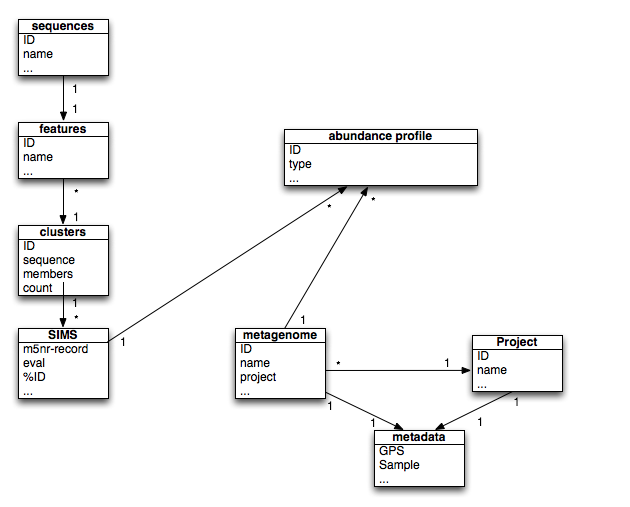
\includegraphics[width=6in]{Images/data-model.png}
\end{center}
\caption{
MG-RAST v3 data model.}
\label{fig:data-model}
\end{figure*}

As shown in Figure \ref{fig:data-model}, MG-RAST relies on abundance profiles to capture information for each metagenome.
The following abundance profiles are calculated for every metagenome.

\begin{itemize}
\item MD5s --
number of sequences (clusters) per database entry in the M5nr.

\item functions --
summary of all the MD5s that match a given function.

\item ontologies --
summary of all the MD5s that match a given hierarchy entry.

\item organisms --
summary of all MD5s that match a given taxon entry.

\item lowest common ancestors
%GWP - anything to say about these?
\end{itemize}

The static helper tables (show in blue in Figure \ref{fig:mgrast_analysis-schema}) help
keep the main tables smaller, by normalizing and providing integer representations for the entities in the abundance profiles.

\begin{figure*}
\begin{center}
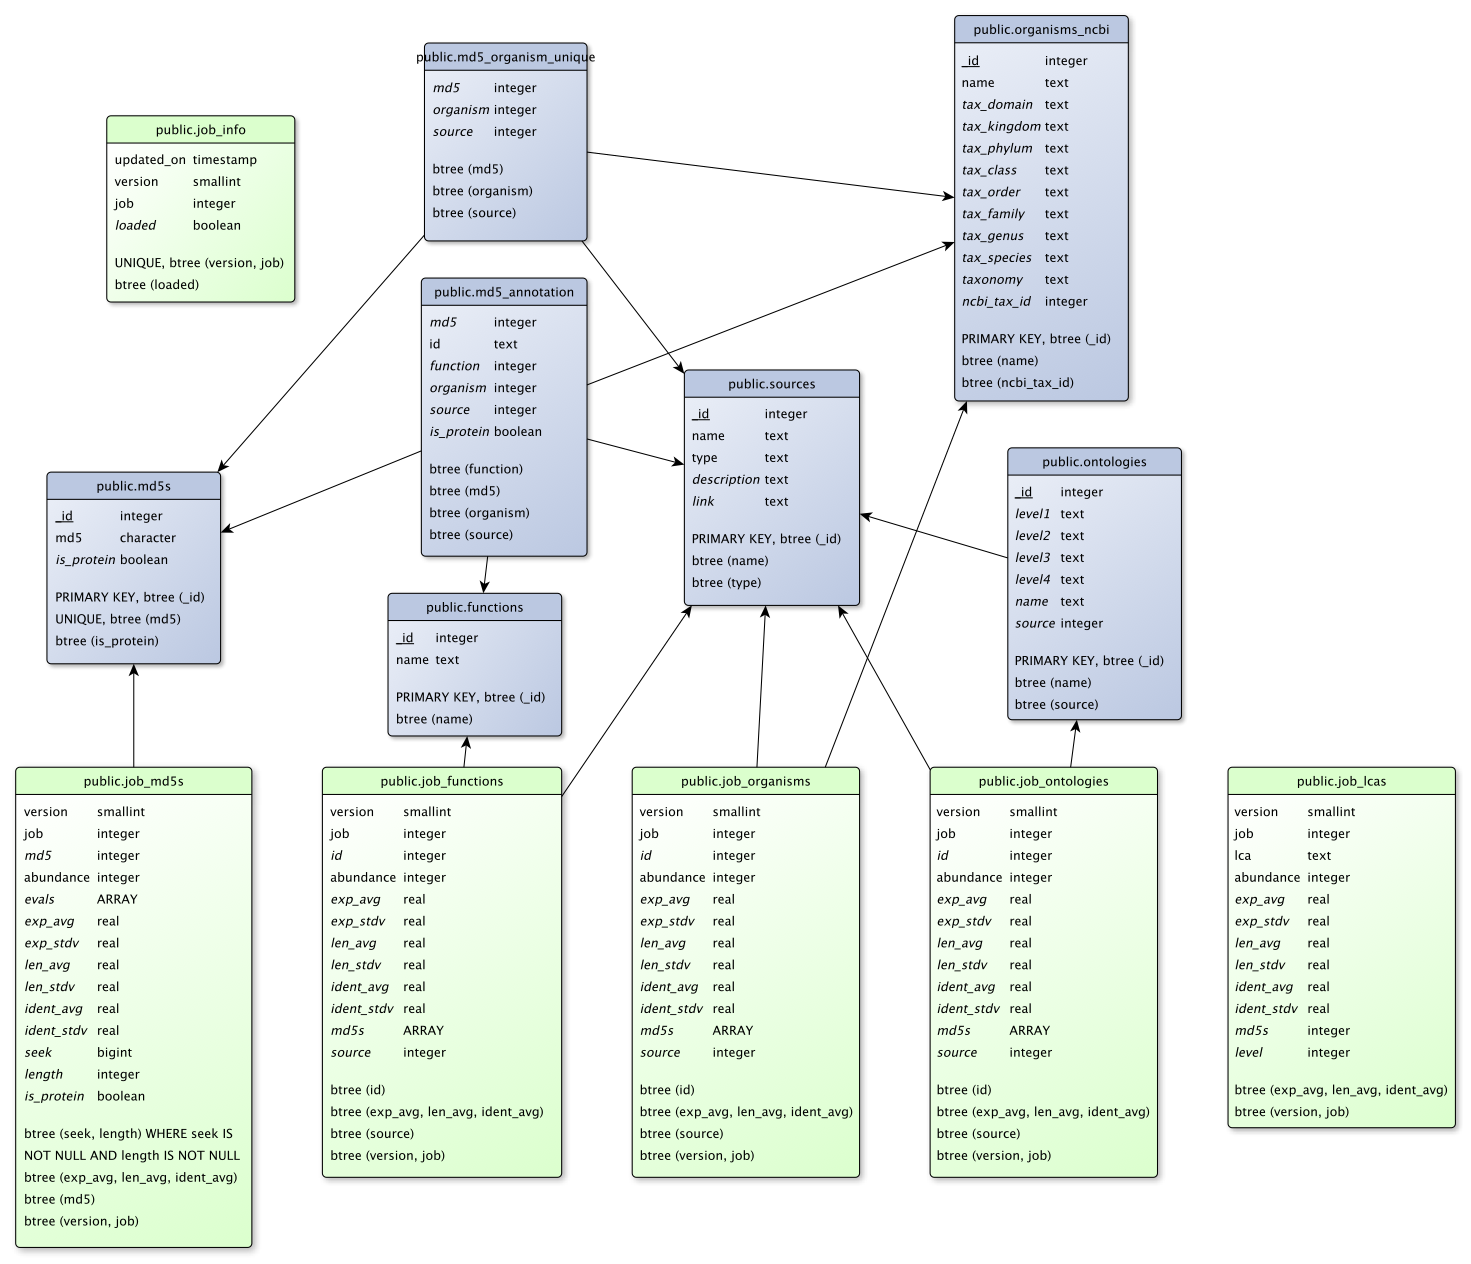
\includegraphics[width=6in]{Images/mgrast_analysis-schema.png}
\end{center}
\caption{
Analysis database schema: static objects (blue) and per metagenome (variable) objects (green).
}
\label{fig:mgrast_analysis-schema}
\end{figure*}

\begin{figure*}
\begin{center}
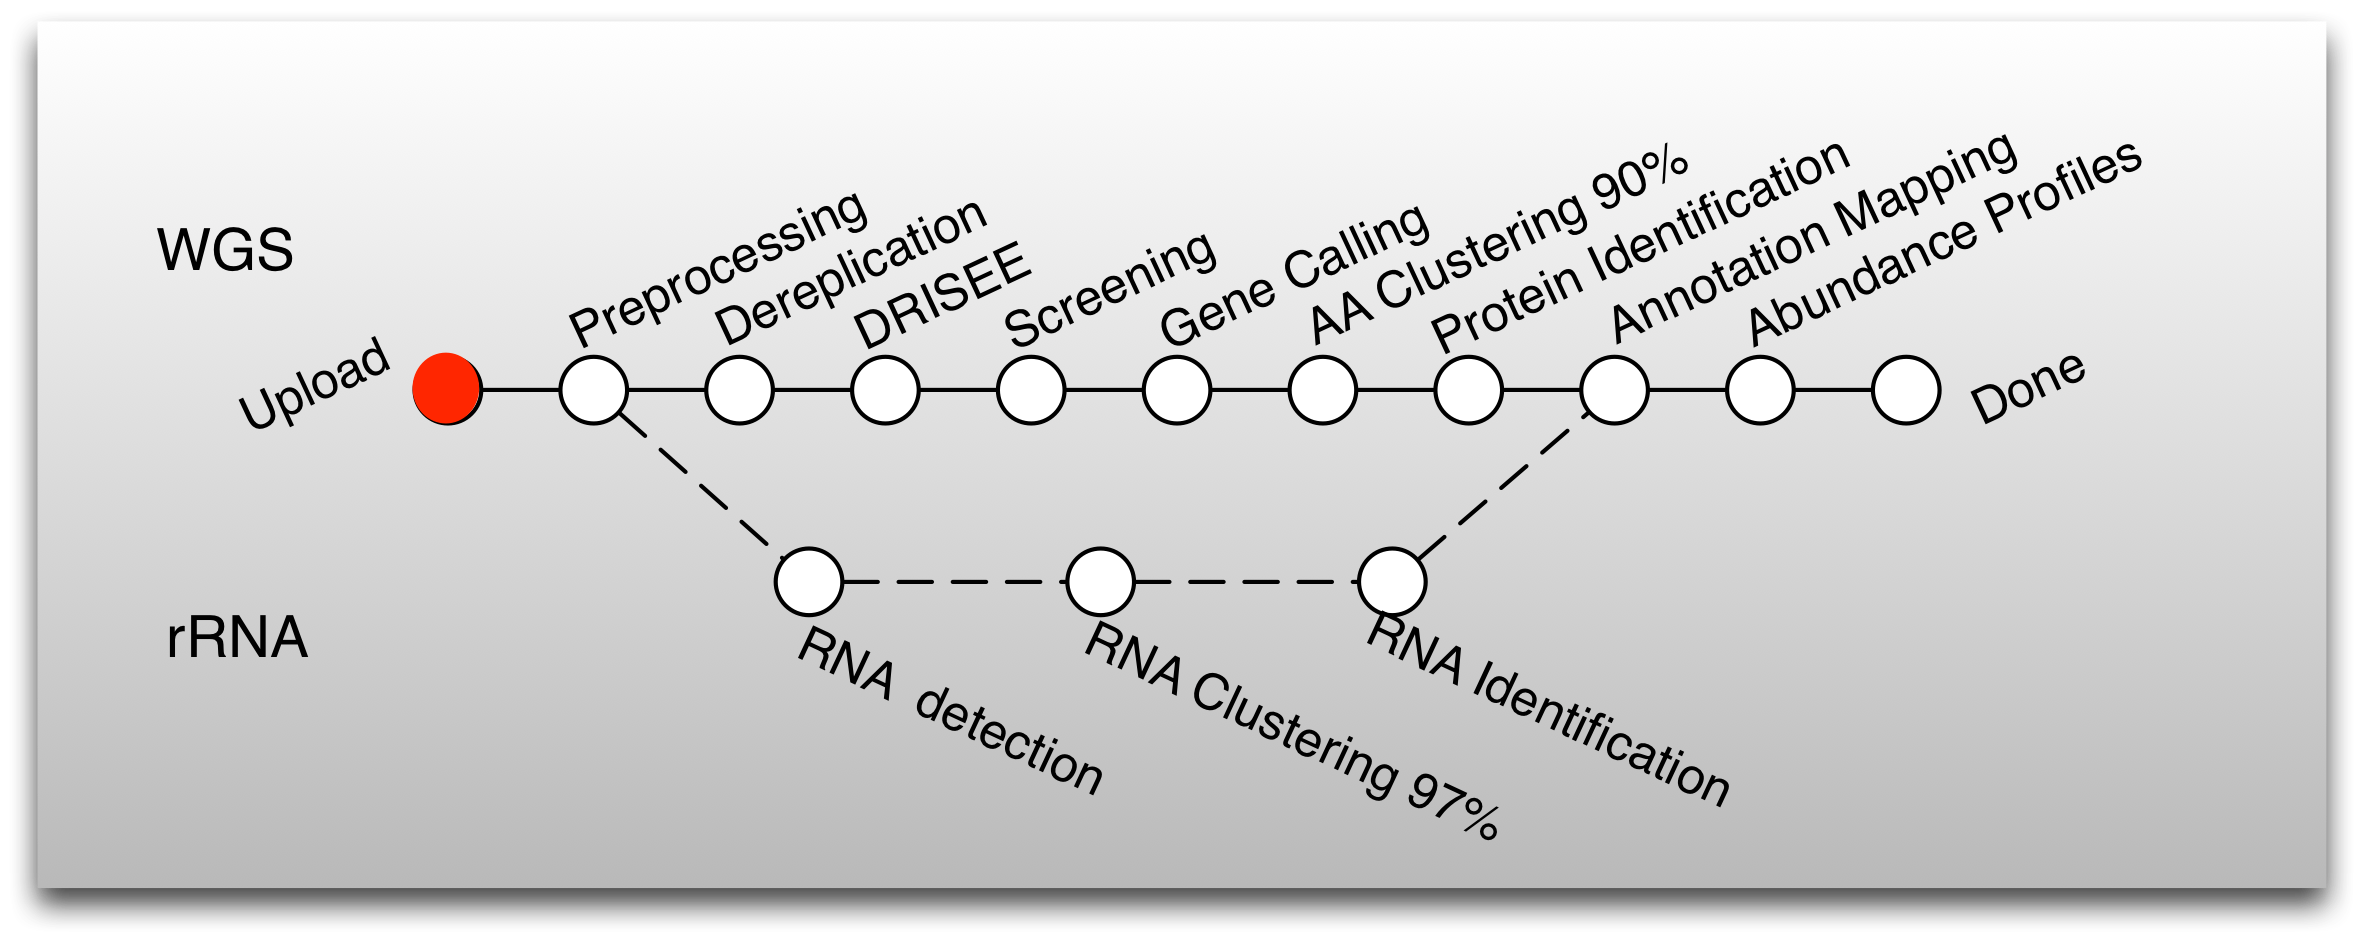
\includegraphics[width=6in]{Images/mgrastv3pipeline.png}
\end{center}
\caption{
Details of the analysis pipeline for MG-RAST version 3}
\label{fig:mgrast-v3-pipeline}
\end{figure*}

% %%%%%%%%%%%%%%%%%%%%%%%%%%%%%%%%%%%%%%%%%%%%%%%%%%%%%%%%%%%%%%%%%%%%%%
% %%%%%%%%%%%%%%%%%%%%%%%%%%%%%%%%%%%%%%%%%%%%%%%%%%%%%%%%%%%%%%%%%%%%%%
% %%%%%%%%%%%%%%%%%%%%%%%%%%%%%%%%%%%%%%%%%%%%%%%%%%%%%%%%%%%%%%%%%%%%%% 
\section{Details on the new MG-RAST pipeline}
\label{section:mgrast_pipeline_details}
The pipeline shown in Figure \ref{fig:mgrast-v3-pipeline} contains a significant number of improvements over version 3.0.
Using the M5nr \cite{M5NR} (an MD5 nonredundant database), the new pipeline computes results against many reference databases instead of only \gls{SEED}.
Several key algorithmic improvements were needed to support the flood of user-generated data (see Figure \ref{fig:mgrast-job-sizes}). Using dedicated software to perform gene prediction instead of using a similarity-based approach reduces runtime requirements. The additional clustering of proteins at 90\% identity reduces data while preserving biological signals.
%Because of the amount of sequence data submitted to MG-RAST (see Figure \ref{fig:mgrast-job-sizes}),
We also restrict the pipeline annotations only to protein coding genes and ribosomal RNA (\gls{rRNA}) genes.

Below we describe each step of the pipeline in some detail. All datasets generated by the individual stages of the processing pipeline are made available as downloads. Appendix \ref{chapter:downloads} lists the available files for each dataset.

\begin{figure*}
\begin{center}
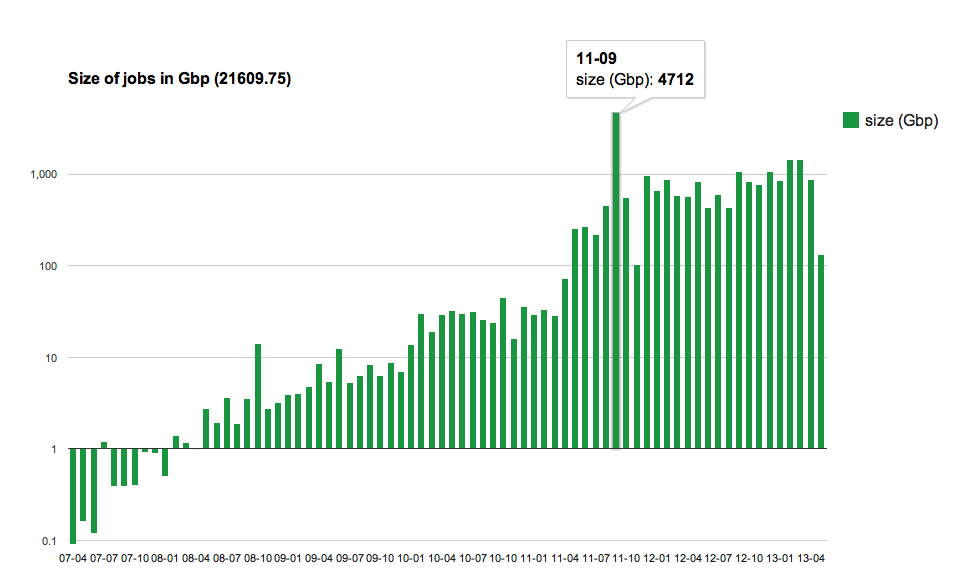
\includegraphics[width=4in]{Images/MG-RAST-job-sizes}
\end{center}
\caption{
Sizes of MG-RAST jobs per month in gigabasepairs from 2007 to 2013.}
\label{fig:mgrast-job-sizes}
\end{figure*}

% %%%%%%%%%%%%%%%%%%%%%%%%%%%%%%%%%%%%%%%%%%%%%%%%%%%%%%%%%%%%%%%%%%%%%%
% %%%%%%%%%%%%%%%%%%%%%%%%%%%%%%%%%%%%%%%%%%%%%%%%%%%%%%%%%%%%%%%%%%%%%%
\subsection{Preprocessing}
After upload, data is preprocessed by using SolexaQA \cite{SOLEXAQA} to trim low-quality regions from FASTQ data. Platform-specific approaches are used for 454 data submitted in FASTA format: reads more than than two standard deviations away from the mean read length are discarded following \cite{HUSEPYRO}. All sequences submitted to the system are available, but discarded reads will not be analyzed further.
% %%%%%%%%%%%%%%%%%%%%%%%%%%%%%%%%%%%%%%%%%%%%%%%%%%%%%%%%%%%%%%%%%%%%%% 
% %%%%%%%%%%%%%%%%%%%%%%%%%%%%%%%%%%%%%%%%%%%%%%%%%%%%%%%%%%%%%%%%%%%%%% 
\subsection{Dereplication}
For shotgun metagenome and shotgun metatranscriptome datasets we perform a dereplication step.
We use a simple k-mer approach to rapidly identify all 20 character prefix identical sequences.
This step is required in order to remove Artificial Duplicate Reads (\gls{ADR}s) \cite{ADRS}. Instead of simply discarding the ADRs, we set them aside and use them later for error estimation.

We note that dereplication is not suitable for amplicon datasets that are likely to share common prefixes.
% %%%%%%%%%%%%%%%%%%%%%%%%%%%%%%%%%%%%%%%%%%%%%%%%%%%%%%%%%%%%%%%%%%%%%% 
% %%%%%%%%%%%%%%%%%%%%%%%%%%%%%%%%%%%%%%%%%%%%%%%%%%%%%%%%%%%%%%%%%%%%%% 
\subsection{DRISEE}
\label{section:DRISEE}
MG-RAST v3 uses DRISEE (Duplicate Read Inferred Sequencing Error Estimation) \cite{DRISEE} to analyze the sets of Artificial Duplicate Reads (\gls{ADR}s) \cite{ADRS} and determine the degree of variation among prefix-identical sequences derived from the same template. See Section \ref{DRISEEDETAIL} for details.

\subsection{Screening}
The pipeline provides the option of removing reads that are near-exact matches to the genomes of a handful of model organisms, including fly, mouse, cow, and human. The screening stage uses Bowtie \cite{BOWTIE} (a fast, memory-efficient, short read aligner), and only reads that do not match the model organisms pass into the next stage of the annotation pipeline.

Note that this option will remove all reads similar to the human genome and render them inaccessible. This decision was made in order to avoid storing any human DNA on MG-RAST.
% %%%%%%%%%%%%%%%%%%%%%%%%%%%%%%%%%%%%%%%%%%%%%%%%%%%%%%%%%%%%%%%%%%%%%%
% %%%%%%%%%%%%%%%%%%%%%%%%%%%%%%%%%%%%%%%%%%%%%%%%%%%%%%%%%%%%%%%%%%%%%% 
\subsection{Gene calling}

The previous version of MG-RAST used similarity-based gene predictions, an approach that is significantly more expensive computationally than de novo gene prediction. After an in-depth investigation of tool performance \cite{TRIMBLE_SHORT}, we have moved to a machine learning approach: FragGeneScan \cite{FGS}. Using this approach, we can now predict coding regions in DNA sequences of 75 bp and longer. Our novel approach also enables the analysis of user-provided assembled contigs.

We note that FragGeneScan is trained for prokaryotes only. While it will identify proteins for eukaryotic sequences, the results should be viewed as more or less random.
% %%%%%%%%%%%%%%%%%%%%%%%%%%%%%%%%%%%%%%%%%%%%%%%%%%%%%%%%%%%%%%%%%%%%%% 
% %%%%%%%%%%%%%%%%%%%%%%%%%%%%%%%%%%%%%%%%%%%%%%%%%%%%%%%%%%%%%%%%%%%%%%
\subsection{AA clustering}
MG-RAST builds clusters of proteins at the 90\% identity level using the uclust \cite{UCLUST} implementation in QIIME \cite{QIIME} preserving the relative abundances. These clusters greatly reduce the computational burden of comparing all pairs of short reads, while clustering at 90\% identity preserves sufficient biological signals.
% %%%%%%%%%%%%%%%%%%%%%%%%%%%%%%%%%%%%%%%%%%%%%%%%%%%%%%%%%%%%%%%%%%%%%% 
% %%%%%%%%%%%%%%%%%%%%%%%%%%%%%%%%%%%%%%%%%%%%%%%%%%%%%%%%%%%%%%%%%%%%%%
\subsection{Protein identification}
Once created, a representative (the longest sequence) for each cluster is subjected to similarity analysis. Instead of BLAST we use sBLAT, an implementation of the BLAT algorithm \cite{BLAT}, which we parallelized using OpenMP \cite{OPENMP} for this work.

Once the similarities are computed, we present reconstructions of the species content of the sample based on the similarity results. We reconstruct the putative species composition of the sample by looking at the phylogenetic origin of the database sequences hit by the similarity searches.
% %%%%%%%%%%%%%%%%%%%%%%%%%%%%%%%%%%%%%%%%%%%%%%%%%%%%%%%%%%%%%%%%%%%%%% 
% %%%%%%%%%%%%%%%%%%%%%%%%%%%%%%%%%%%%%%%%%%%%%%%%%%%%%%%%%%%%%%%%%%%%%%
\subsection{Annotation mapping}
 Sequence similarity searches are computed against a protein database derived from the M5nr \cite{M5NR}, which provides nonredundant integration of many databases: GenBank,\cite{GENBANK}, \gls{SEED} \cite{SUBSYSTEMS}, IMG \cite{IMG}, UniProt \cite{UNIPROT}, KEGG \cite{KEGG}, and eggNOGs \cite{EGGNOG}. Unlike MG-RAST v2, which relied solely on SEED, MG-RAST now supports many complementary views into the data with one similarity search, including different functional hierarchies: SEED \gls{Subsystem}s, IMG terms, COG \cite{COG}, eggNOGs \cite{EGGNOG}, and ontologies such as GO (Gene Ontology Consortium, 2013). Users can easily change views without recomputation. For example, COG and KEGG views can be displayed, which both show the relative abundances of histidine biosynthesis in a dataset of four cow rumen metagenomes.
% %%%%%%%%%%%%%%%%%%%%%%%%%%%%%%%%%%%%%%%%%%%%%%%%%%%%%%%%%%%%%%%%%%%%%%
% %%%%%%%%%%%%%%%%%%%%%%%%%%%%%%%%%%%%%%%%%%%%%%%%%%%%%%%%%%%%%%%%%%%%%% 
\subsection{Abundance profiles}

Abundance profiles are the primary data product that MG-RAST's user interface uses to display information on the datasets.
%Abundance profiles functional and taxonomic information.

Using the abundance profiles, the MG-RAST system defers making a decision on when to transfer annotations. Since there is no well-defined threshold that is acceptable for all use cases, the abundance profiles contain all similarities and require their users to set cut-off values.

The threshold for annotation transfer can be set by using the following parameters:
e-value,
percent identity, and
minimal alignment length.

The taxonomic profiles use the NCBI taxnomy. All taxonomic information is projected against this data.
The functional profiles are available for data sources that provide hierarchical information. These currently comprise the following.

\begin{itemize}
\item \gls{SEED} \gls{Subsystem}s

The SEED subsystems\cite{SUBSYSTEMS} represent an independent reannotation effort that powers, for example,  the RAST\cite{RAST} effort. Manual curation of subsystems makes them an extremely valuable data source.

Subsystems represent a four-level hierarchy:
\begin{enumerate}
\item Subsystem level 1 -- highest level
\item Subsystem level 2 -- 
\item Subsystem level 3 -- similar to a KEGG pathway
\item Subsystem level 4 -- actual functional assignment to the feature in question
\end{enumerate}

The page at \url{http://pubseed.theseed.org/SubsysEditor.cgi} allows browsing the subsystems.

\item KEGG Orthologs

We use the KEGG\cite{KEGG} enzyme number hierarchy to implement a four-level hierarchy.
\begin{enumerate}
\item KEGG level 1 -- first digit of the EC number (EC:X.*.*.*)
\item KEGG level 2 -- first two digits of the EC number (EC:X.Y.*.*)
\item KEGG level 3 -- first three digits of the EC number (EC:X:Y:Z:.*)
\item KEGG level 4 -- entire four digits EC number
\end{enumerate}

We note that KEGG data is no longer available for free download. We thus have to rely on using the latest freely downloadable version of the data.

The high-level KEGG categories are as follows.
\begin{enumerate}
\item Cellular Processes
\item Environmental Information Processing
\item Genetic Information Processing
\item Human Diseases
\item Metabolism
\item Organizational Systems
\end{enumerate}

\item COG and EGGNOG Categories

The high-level COG and EGGNOG categories are as follows.
\begin{enumerate}
\item Cellular Processes
\item Information Storage and Processing
\item Metabolism
\item Poorly Characterized
\end{enumerate}

We note that for most metagenomes the coverage of each of the four namespaces is quite different. The ``source hits distribution" (see Section \ref{section:source-hits-distribution}) provides information on how many sequences per dataset
were found for each database.
\end{itemize}
% %%%%%%%%%%%%%%%%%%%%%%%%%%%%%%%%%%%%%%%%%%%%%%%%%%%%%%%%%%%%%%%%%%%%%% 
% %%%%%%%%%%%%%%%%%%%%%%%%%%%%%%%%%%%%%%%%%%%%%%%%%%%%%%%%%%%%%%%%%%%%%% 
% %%%%%%%%%%%%%%%%%%%%%%%%%%%%%%%%%%%%%%%%%%%%%%%%%%%%%%%%%%%%%%%%%%%%%% 
\section{The rRNA pipeline}

\gls{rRNA} reads are identified by using a simple rRNA detection pipeline and are searched in a separate flow in the pipeline.
% %%%%%%%%%%%%%%%%%%%%%%%%%%%%%%%%%%%%%%%%%%%%%%%%%%%%%%%%%%%%%%%%%%%%%%
\subsection{rRNA detection}
An initial BLAT \cite{BLAT} search against a reduced RNA database efficiently identifies RNA. The reduced database is a 90\% identity clustered version of the SILVA database and is used to rapidly identify sequences with similarities to ribosomal RNA.

%\textbf{ANDREAS how is this DB built!}

% %%%%%%%%%%%%%%%%%%%%%%%%%%%%%%%%%%%%%%%%%%%%%%%%%%%%%%%%%%%%%%%%%%%%%%
\subsection{rRNA clustering}
The rRNA-similar reads are then clustered at 97\% identity, and the longest sequence is picked as the cluster representative.
% %%%%%%%%%%%%%%%%%%%%%%%%%%%%%%%%%%%%%%%%%%%%%%%%%%%%%%%%%%%%%%%%%%%%%%
\subsection{rRNA identification}
 A BLAT similarity search for the longest cluster representative is performed against the M5rna database which integrates SILVA\cite{SILVA}, Greengenes\cite{GREENGENES}, and RDP\cite{RDP}.
% %%%%%%%%%%%%%%%%%%%%%%%%%%%%%%%%%%%%%%%%%%%%%%%%%%%%%%%%%%%%%%%%%%%%%% 
% %%%%%%%%%%%%%%%%%%%%%%%%%%%%%%%%%%%%%%%%%%%%%%%%%%%%%%%%%%%%%%%%%%%%%% 
% %%%%%%%%%%%%%%%%%%%%%%%%%%%%%%%%%%%%%%%%%%%%%%%%%%%%%%%%%%%%%%%%%%%%%% 
\section{Quality assessment}
\label{section:Quality}
The MG-RAST pipeline offers a variety of summaries of technical aspects of the sequence quality to enable sequence data triage.  These tools include DRISEE for estimating sequence error, summaries of the spectra of long kmers, and visualizations of the base caller output.
% %%%%%%%%%%%%%%%%%%%%%%%%%%%%%%%%%%%%%%%%%%%%%%%%%%%%%%%%%%%%%%%%%%%%%% 
% %%%%%%%%%%%%%%%%%%%%%%%%%%%%%%%%%%%%%%%%%%%%%%%%%%%%%%%%%%%%%%%%%%%%%% 
\subsection{DRISEE}
\label{DRISEEDETAIL}

DRISEE \cite{DRISEE} is a method for measuring sequencing error in whole-genome shotgun metagenomic sequence data that is independent of sequencing technology and overcomes many of the shortcomings of Phred. It utilizes artificial duplicate reads (ADRs) to generate internal sequence standards from which an overall assessment of sequencing error in a sample is derived. 
The current implementation of DRISEE is not suitable for amplicon sequencing data or other samples that may contain natural duplicated sequences (e.g., eukaryotic DNA where gene duplication and other forms of highly repetitive sequences are common) in high abundance.
\
%DRISEE values are normally reported as percent error.
%DRISEE values can be used to assess the overall quality of sequence samples.
DRISEE results are presented on the Overview page for each MG-RAST sample for which a DRISEE profile can be determined.
Total DRISEE error presents the overall DRISEE-based assessment of the sample as a percent error:

\begin{small}
$$Total \,\, DRISEE \,\, Error = \frac{base\_errors}{total\_bases} * 100$$
\end{small}

\noindent where ${base\_errors}$ refers to the sum of DRISEE-detected errors and ${total\_bases}$ refers to the sum of all bases considered by DRISEE.
Beneath the Total DRISEE Error, a barchart indicates the error for the sample (the red vertical bar) as well as the minimum (barchart initial value), maximum (barchart final value), mean \begin{math}(\mu)\end{math}, mean +/- one standard deviation (\begin{math}\sigma\end{math}), and mean +/- two standard deviations (\begin{math}2\sigma\end{math}) Total DRISEE Errors observed among all samples in MG-RAST for which a DRISEE profile has been computed. 

The DRISEE plot presents a more detailed view of the DRISEE profile; the DRISEE percent error is displayed per base. Individual errors (A,T,C,G, and N substitution rates as well as the InDel rate) are presented as well as a cumulative total.

Users can download DRISEE values as a tab-separated file. The first line of the file contains headers for the values in the second line. The second line contains DRISEE percent error values for A substitutions (A\_err), T substitutions (T\_err), C substitutions (C\_err), G substitutions (G\_err), N substitutions (N\_err), insertions and deletions (InDel\_err), and the Total DRISEE Error. The third line indicates headers for all remaining lines. Rows 4 and 4+ present the DRISEE counts for the indexed position across all considered bins of ADRs. Column values represent the number of reads that match an A,T,C,G,N, or InDel at the indicated position relative to the appropriate consensus sequence followed by the number of reads that do not match an A,T,C,G,N, or InDel.
% %%%%%%%%%%%%%%%%%%%%%%%%%%%%%%%%%%%%%%%%%%%%%%%%%%%%%%%%%%%%%%%%%%%%%% 
% %%%%%%%%%%%%%%%%%%%%%%%%%%%%%%%%%%%%%%%%%%%%%%%%%%%%%%%%%%%%%%%%%%%%%% 
\subsection{Kmer profiles}

kmer digests are an annotation-independent method for describing sequence datasets that can support inferences about genome size and coverage. Here the Overview page presents several visualizations, evaluated at k=15:
%Three visualizations provided of the kmer spectrum are 
the kmer spectrum, kmer rank abundance, and ranked kmer consumed. All three graphs represent the same spectrum, but in different ways. The kmer spectrum plots the number of distinct kmers against kmer coverage; the kmer coverage is equivalent to number of observations of each kmer. The kmer rank abundance plots the relationship between kmer coverage and the kmer rank� answering the question ``What is the coverage of the nth most-abundant kmer?". Ranked kmer consumed plots the largest fraction of the data explained by the nth most-abundant kmers only.

\subsection{Nucleotide histograms}

Nucleotide histograms are graphs showing the fraction of base pairs of each type (A, C, G, T, or ambiguous base ``N") at each position starting from the beginning of each read.

Amplicon datasets (see Figure \ref{fig:nucleotide-hist-amplicon}) should show biased distributions of bases at each position, reflecting both conservation and variability in the recovered sequences:

\begin{figure}[ht]
\begin{center}
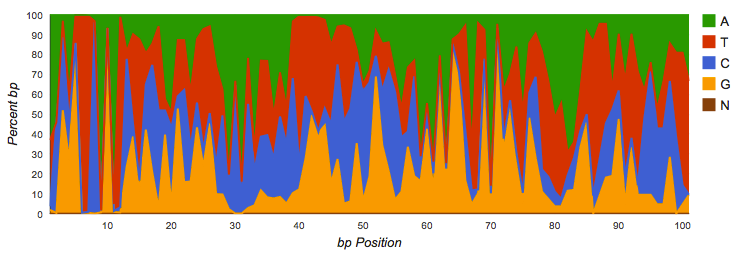
\includegraphics[width=4in]{Images/nucleotide-hist-amplicon.png}
\end{center}
\caption{
 Nucleotide histogram with biased distributions typical for an amplicon dataset.}
\label{fig:nucleotide-hist-amplicon}
\end{figure}

Shotgun datasets should have roughly equal proportions of A, T, G and C basecalls, independent of position in the read as shown in Figure \ref{fig:nucleotide-hist-ok}.

\begin{figure}[ht]
\begin{center}
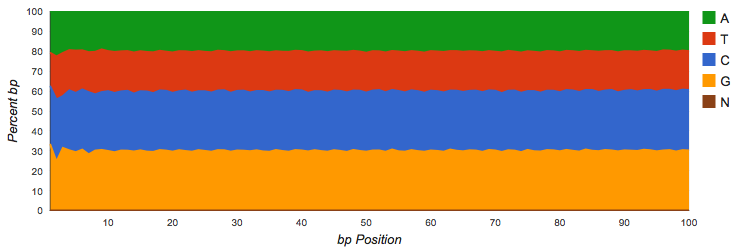
\includegraphics[width=4in]{Images/nucleotide-hist-ok.png}
\end{center}
\caption{
Nucleotide histogram showing ideal distributions typical for a shotgun metagenome.
}
\label{fig:nucleotide-hist-ok}
\end{figure}

Vertical bars at the beginning of the read indicate untrimmed (see Figure \ref{fig:nucleotide-hist-barcodes}), contiguous barcodes. Gene calling via FragGeneScan \cite{FGS} and \gls{RNA} similarity searches are not impacted by the presence of barcodes. However, if a significant fraction of the reads is consumed by barcodes, it reduces the biological information contained in the reads.

\begin{figure}[ht]
\begin{center}
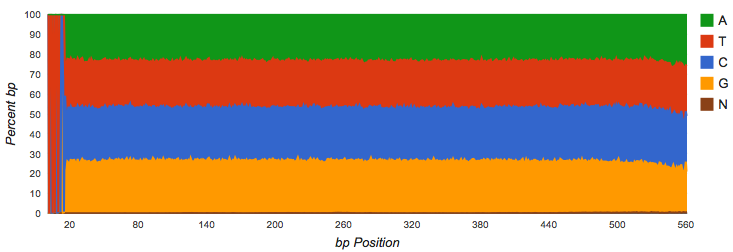
\includegraphics[width=4in]{Images/nucleotide-hist-barcodes.png}
\end{center}
\caption{
Nucleotide histogram with untrimmed barcodes.
}
\label{fig:nucleotide-hist-barcodes}
\end{figure}

If a shotgun dataset has clear patterns in the data, these indicate likely contamination with artificial sequences.
The dataset shown in see Figure \ref{fig:nucleotide-with-contamination} had a large fraction of adapter dimers.

\begin{figure}
\begin{center}
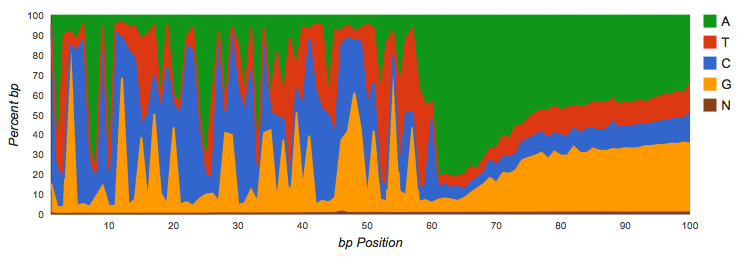
\includegraphics[width=4in]{Images/nucleotide-with-contamination.png}
\end{center}
\caption{
Nucleotide histogram with contamination.
}
\label{fig:nucleotide-with-contamination}
\end{figure}
% %%%%%%%%%%%%%%%%%%%%%%%%%%%%%%%%%%%%%%%%%%%%%%%%%%%%%%%%%%%%%%%%%%%%%% 
% %%%%%%%%%%%%%%%%%%%%%%%%%%%%%%%%%%%%%%%%%%%%%%%%%%%%%%%%%%%%%%%%%%%%%% 
% %%%%%%%%%%%%%%%%%%%%%%%%%%%%%%%%%%%%%%%%%%%%%%%%%%%%%%%%%%%%%%%%%%%%%%
\section{Best hit, representative hit, and lowest common ancestor interpretation}
\label{section:hit-types}

MG-RAST searches the nonredundant M5nr and M5rna databases in which each sequence is unique. These two databases are built from multiple sequence database sources, and the individual sequences may occur multiple times in different strains and species (and sometimes genera) with 100\% identity. In these circumstances, choosing the ``right'' taxonomic information is not a straightforward process.

To optimally serve a number of different use cases, we have implemented three methods--best hit, representative hit, and lowest common ancestor---for 
end users to determine the number of hits
(occurrences of the input sequence in the database)
reported for a given sequence in their dataset.
%Details about the three different classification functions implemented are given below.
% %%%%%%%%%%%%%%%%%%%%%%%%%%%%%%%%%%%%%%%%%%%%%%%%%%%%%%%%%%%%%%%%%%%%%% 
% %%%%%%%%%%%%%%%%%%%%%%%%%%%%%%%%%%%%%%%%%%%%%%%%%%%%%%%%%%%%%%%%%%%%%%
\subsection{Best hit}

The best hit classification reports the functional and taxonomic annotation of the best hit in the M5nr for each feature. In those cases where the similarity search yields multiple same-scoring hits for a feature, we do not choose any single ``correct'' label. For this reason we have decided to double count all annotations with identical match properties and leave determination of truth to our users. While this approach aims to inform about the functional and taxonomic potential of a microbial community by preserving all information, subsequent analysis can be biased because of a single feature having multiple annotations, leading to inflated hit counts. For users looking for a specific species or function in their results, the best hit classification is likely what is wanted.
% %%%%%%%%%%%%%%%%%%%%%%%%%%%%%%%%%%%%%%%%%%%%%%%%%%%%%%%%%%%%%%%%%%%%%% 
% %%%%%%%%%%%%%%%%%%%%%%%%%%%%%%%%%%%%%%%%%%%%%%%%%%%%%%%%%%%%%%%%%%%%%%
\subsection{Representative hit}

The representative hit classification selects a single, unambiguous annotation for each feature. The annotation is based on the first hit in the homology search and the first annotation for that hit in our database. This approach makes counts additive across functional and taxonomic levels and thus allows, for example, the comparison of functional and taxonomic profiles of different metagenomes.
% %%%%%%%%%%%%%%%%%%%%%%%%%%%%%%%%%%%%%%%%%%%%%%%%%%%%%%%%%%%%%%%%%%%%%% 
% %%%%%%%%%%%%%%%%%%%%%%%%%%%%%%%%%%%%%%%%%%%%%%%%%%%%%%%%%%%%%%%%%%%%%%
\subsection{Lowest Common Ancestor (LCA)}
\label{section:LCA}
To avoid the problem of multiple taxonomic annotations for a single feature, we provide taxonomic annotations based on the widely used LCA method introduced by MEGAN \cite{MEGAN}. In this method all hits are collected that have a bit score close to the bit score of the best hit. The taxonomic annotation of the feature is then determined by computing the LCA of all species in this set. This replaces all taxonomic annotations from ambiguous hits with a single higher-level annotation in the NCBI taxonomy tree.
% %%%%%%%%%%%%%%%%%%%%%%%%%%%%%%%%%%%%%%%%%%%%%%%%%%%%%%%%%%%%%%%%%%%%%% 
% %%%%%%%%%%%%%%%%%%%%%%%%%%%%%%%%%%%%%%%%%%%%%%%%%%%%%%%%%%%%%%%%%%%%%% 
\subsection{Comparison of methods}
Users should be aware that the number of hits might be inflated if the best hit filter is used or that a favorite species might be missing despite a similar sequence similarity result if the representative hit filter is used (in fact, even if a 100\% identical match to a favorite species exists).

One way to consider both the best hit and representative hit is that they overinterpret the available evidence. With the LCA classifier function, on the other hand, any input sequence is classified only down to a trustworthy taxonomic level. While naively this seems to be the best function to choose in all cases because it classifies sequences to varying depths, the approach causes problems for downstream analysis tools that might rely on everything being classified to the same level.
% %%%%%%%%%%%%%%%%%%%%%%%%%%%%%%%%%%%%%%%%%%%%%%%%%%%%%%%%%%%%%%%%%%%%%% 
% %%%%%%%%%%%%%%%%%%%%%%%%%%%%%%%%%%%%%%%%%%%%%%%%%%%%%%%%%%%%%%%%%%%%%% 
%%%%%%%%%%%%%%%%%%%%%%%%%%%%%%%%%%%%%%%%%%%%%%%%%%%%%%%%%%%%%%%%%%%
\section{Numbers of annotations vs. number of reads}
\label{section:annotation_numbers}
The MG-RAST v3 annotation pipeline does not usually provide a single annotation for each submitted fragment of DNA. Steps in the pipeline map one read to multiple annotations and one annotation to multiple reads. These steps are a consequence of genome structure, pipeline engineering, and the character of the sequence databases that MG-RAST uses for annotation.

The first step that is not one-to-one is gene prediction. Long reads ($>$ $400$bp) and contigs can contain pieces of two or more microbial genes; when the gene caller makes this prediction, the multiple predicted protein sequences (called fragments) are annotated separately.

An intermediate clustering step identifies sequences at 90\% amino acid identity and performs one search for each cluster. Sequences that do not fall into clusters are searched separately. The ``abundance'' column in the MG-RAST tables presents the estimate of the number of sequences that contain a given annotation, found by multiplying each selected database match (hit) by the number of representatives in each cluster.
The final step that is not one-to-one is the annotation process itself. Sequences can exist in the underlying data sources many times with different labels. When those sequence are the best hit similarity, we do not have a principled way to choosing the ``correct'' label. For this reason we have decided to double count these annotations and leave determination of truth to our users. Note: Even when considering a single data source, double-counting can occur depending on the consistency of annotations.
Also note: Hits refer to the number of unique database sequences that were found in the similarity search, {\bf not} the number of reads. The hit count can be smaller than the number of reads because of clustering or larger due to double counting.
% %%%%%%%%%%%%%%%%%%%%%%%%%%%%%%%%%%%%%%%%%%%%%%%%%%%%%%%%%%%%%%%%%%%%%%
% %%%%%%%%%%%%%%%%%%%%%%%%%%%%%%%%%%%%%%%%%%%%%%%%%%%%%%%%%%%%%%%%%%%%%%
% %%%%%%%%%%%%%%%%%%%%%%%%%%%%%%%%%%%%%%%%%%%%%%%%%%%%%%%%%%%%%%%%%%%%%% 
\section{Metadata}
\label{section:metadata}

MG-RAST is both an analytical platform and a data integration system. To enable data reuse, for example for meta-analyses, we require that all data being made publicly available to third parties contain at least minimal metadata. The MG-RAST team has decided to follow the minimal checklist approach used by the Genomics Standards Consortium (GSC)\cite{GSC}.

While the GSC provides a GCDML \cite{GCDML} encoding, this XML-based format is more useful to programmers than to end users submitting data.
We have therefore elected to use spreadsheets to transport metadata. Specifically we use MIxS (Minimum information about any (x) sequence (MIxS) and MIMARKS (Minimum Information about a MARKer gene Survey) to encode minimal metadata \cite{MIENS}.

The metadata describe the origins of samples and provide details on the generation of the sequence data. While the GSC checklist aims at capturing a minimum of information, MG-RAST can handle additional metadata if supplied by the user. The metadata is stored in a simple key value format and is displayed on the Metagenome Overview page.

Once uploaded, the metadata spreadsheets are validated automatically, and users are informed of any problems.

The presence of metadata enables discovery by end users using contextual metadata. Users can perform searches such as ``retrieve soil samples from the continental U.S.A.'' If the users have added additional metadata (domain specific extension), additional queries are enabled: for example, ``restrict the results to soils with a specific pH".
% %%%%%%%%%%%%%%%%%%%%%%%%%%%%%%%%%%%%%%%%%%%%%%%%%%%%%%%%%%%%%%%%%%%%%%
% %%%%%%%%%%%%%%%%%%%%%%%%%%%%%%%%%%%%%%%%%%%%%%%%%%%%%%%%%%%%%%%%%%%%%%
% %%%%%%%%%%%%%%%%%%%%%%%%%%%%%%%%%%%%%%%%%%%%%%%%%%%%%%%%%%%%%%%%%%%%%% 
% %%%%%%%%%%%%%%%%%%%%%%%%%%%%%%%%%%%%%%%%%%%%%%%%%%%%%%%%%%%%%%%%%%%%%%
% %%%%%%%%%%%%%%%%%%%%%%%%%%%%%%%%%%%%%%%%%%%%%%%%%%%%%%%%%%%%%%%%%%%%%%
\chapter{MG-RAST v3 web interface}

The MG-RAST system provides a rich web user interface that covers all aspects of the metagenome analysis, from data upload to ordination analysis. The web interface can also be used for data discovery. Metagenomic datasets can be easily selected individually or on the basis of filters such as technology (including read length), quality, sample type, and keyword, with dynamic filtering of results based on similarity to known reference proteins or taxonomy. For example, a user might want to perform a search such as ``phylum eq `actinobacteria' and function in `KEGG pathway Lysine Biosynthesis'� and sample in `Ocean'" to extract sets of reads matching the appropriate functions and taxa across metagenomes. The results can be displayed in familiar formats, including bar charts, trees that incorporate abundance information, heatmaps, or principal components analyses, or exported in tabular form. The raw or processed data can be recovered via download pages. Metabolic reconstructions based on mapping to KEGG pathways are also provided.

Sample selection is crucial for understanding large-scale patterns when multiple metagenomes are compared. Accordingly, MG-RAST supports MIxS and MIMARKS (Yilmaz, 2011) (as well as domain-specific plug-ins for specialized environments not extending the minimal GSC standards); several projects, including TerraGenome, HMP, TARA, and EMP, use these GSC standards, enabling standardized queries that integrate new samples into these massive datasets. An example query using the metadata browser, enabling the user to interrogate the existing pool of public datasets for a biome of interest (e.g., hot springs) and performing comparisons and a search for organisms encoding a specific gene function (e.g., beta-lactamase or aldo/keto reductase) is given in
Figure \ref{fig:quad-chart-analysis-example}.

One key aspect of the MG-RAST approach is the creation of smart data products enabling the user at the time of analysis to determine the best parameters for, for example, a comparison between samples. This is done without the need for recomputation of results.

\begin{figure*}
\begin{center}
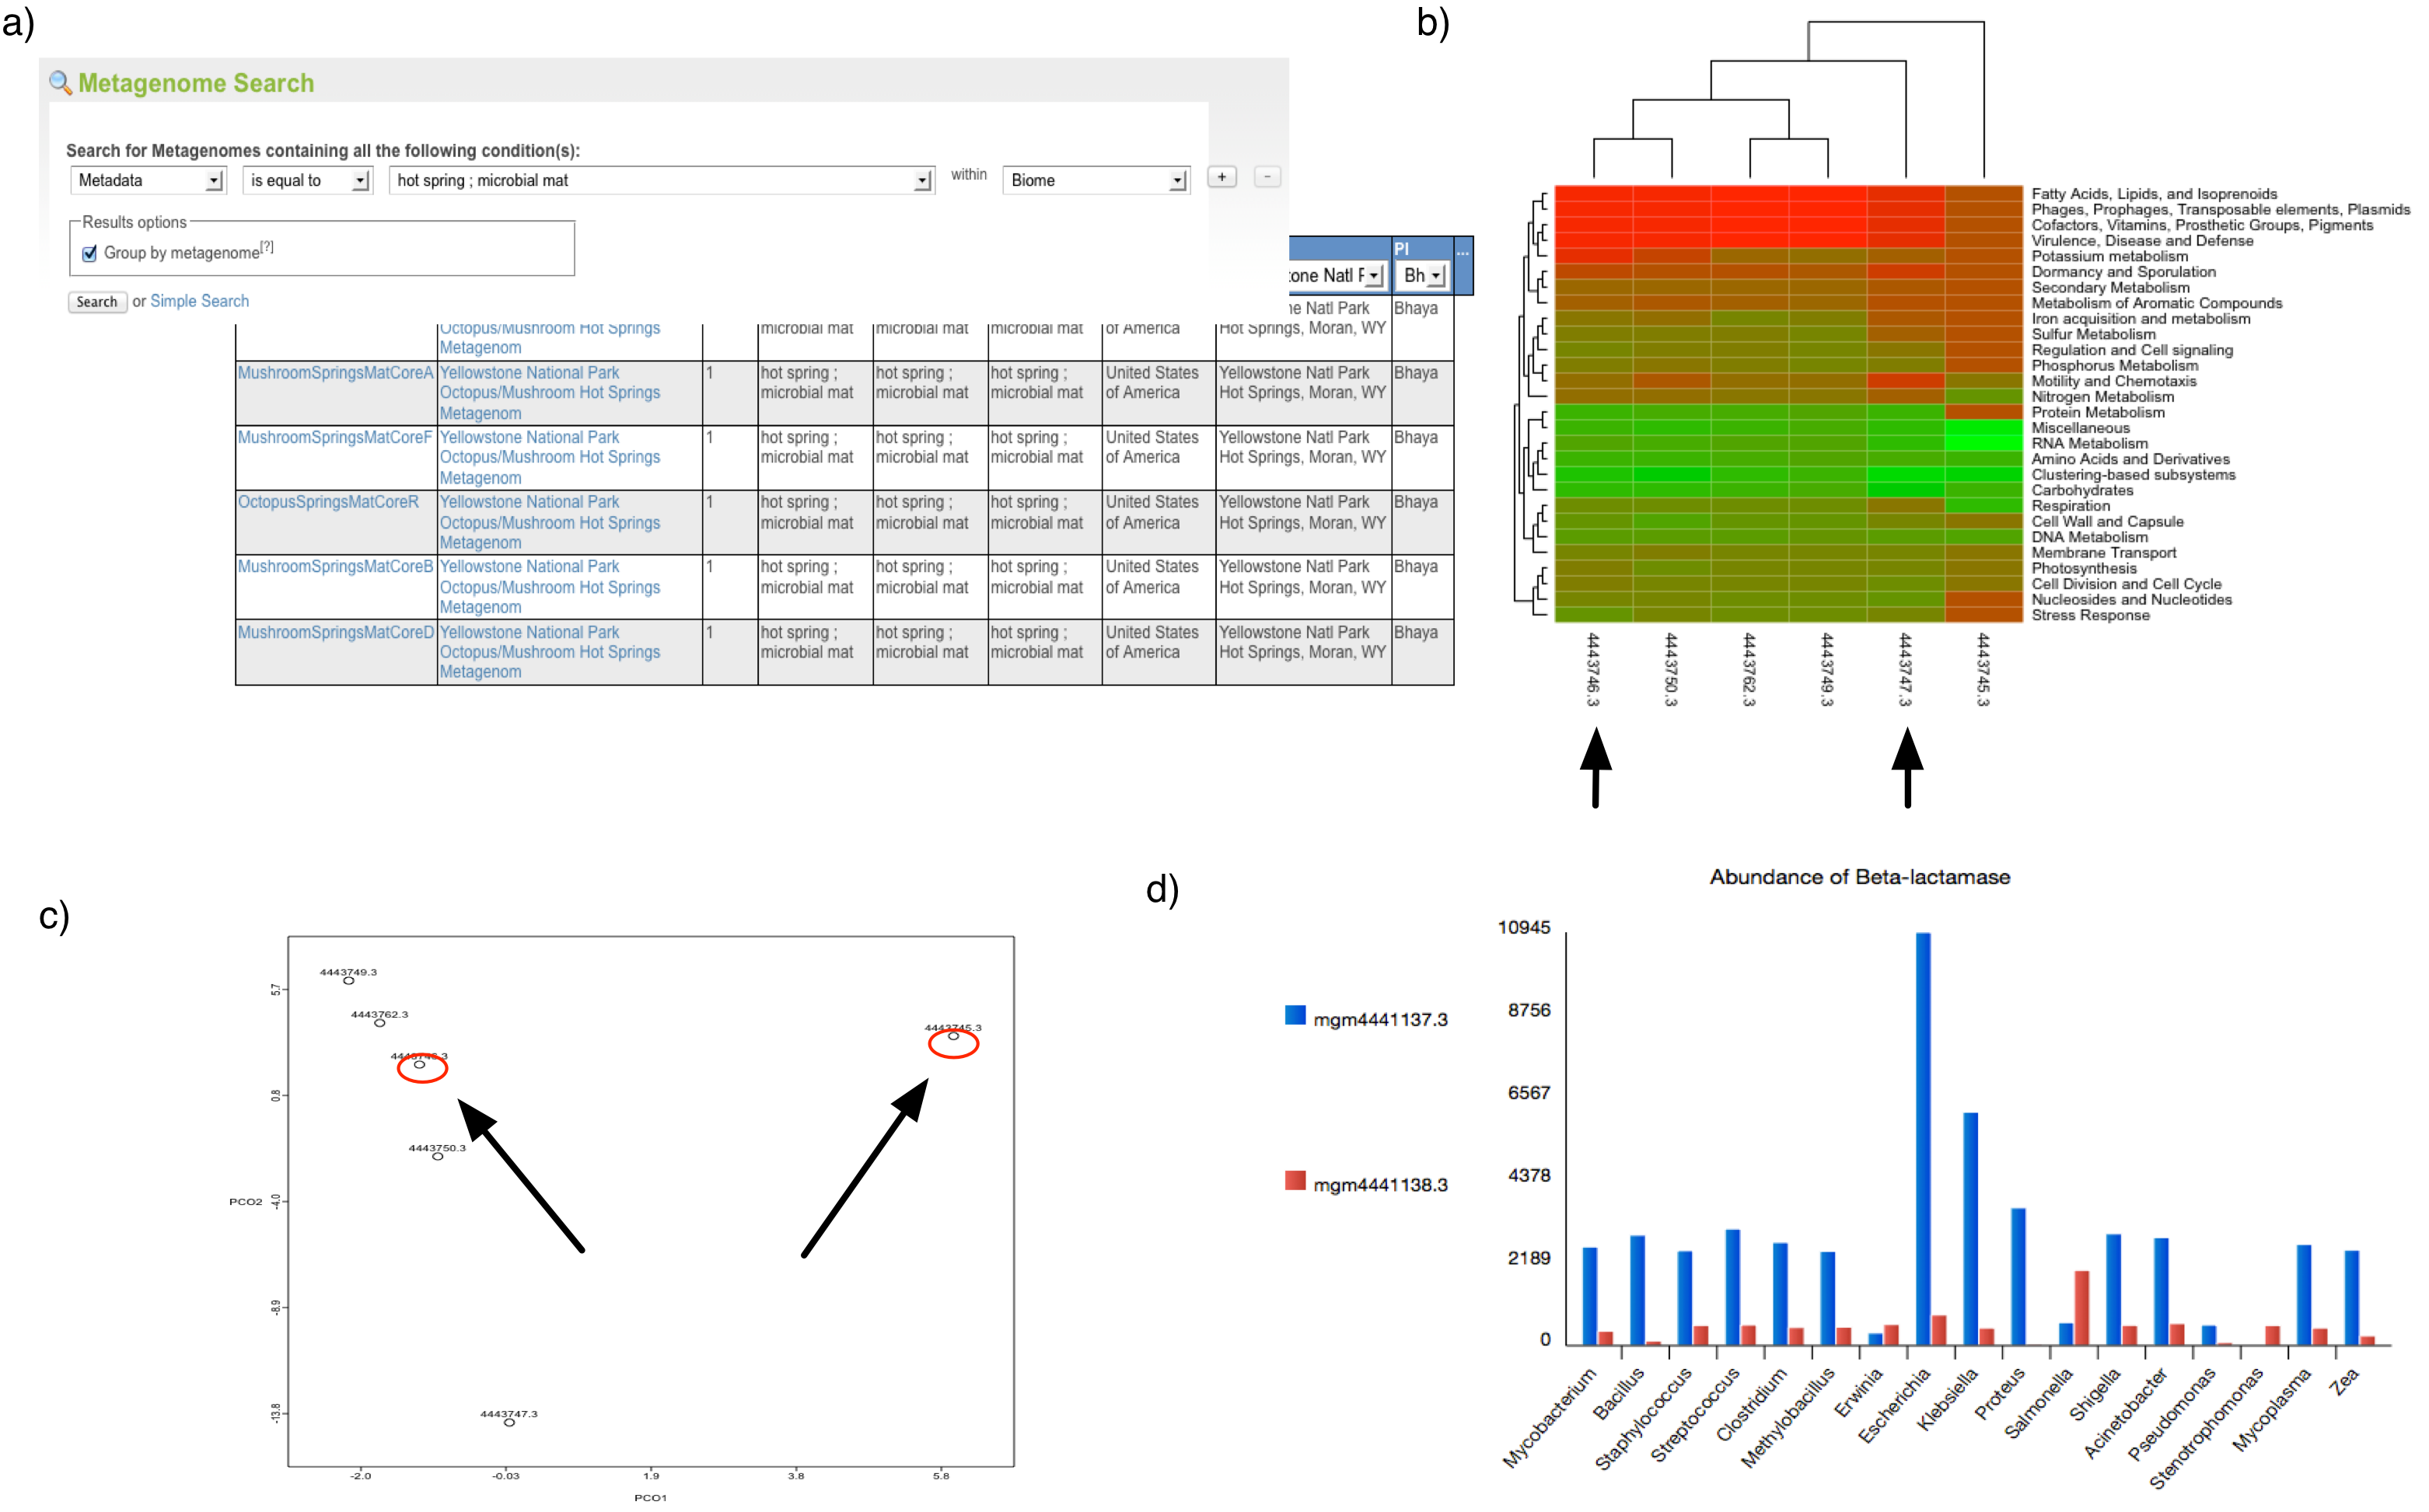
\includegraphics[width=6in]{Images/quad-chart-analysis-example.png}
\end{center}
\caption{
(a) Using the web interface for a search of metagenomes for microbial mats in hotsprings (GSC-MIMS-Keywords Biome=``hotspring; microbial mat"), we find 6 metagenomes (refs: 4443745.3, 4443746.3, 4443747.3, 4443749.3, 4443750.3, 4443762.3). (b) Initial comparison reveals some differences in protein functional class abundance (using \gls{SEED} subsystens level 1). (c) From the PCoA plot using normalized counts of functional \gls{SEED} \gls{Subsystem}--based functional annotations (level 2) and Bray-Curtis as metric, we attempt to find differences between two similar datasets (MG-RAST-IDs: 444749.3, 4443762.3). (d) Using exported tables with functional annotations and taxonomic mapping, we analyze the distribution of organisms observed to contain beta-lactamase and plot the abundance per species for two distinct samples.
}
\label{fig:quad-chart-analysis-example}
\end{figure*}
% %%%%%%l%%%%%%%%%%%%%%%%%%%%%%%%%%%%%%%%%%%%%%%%%%%%%%%%%%%%%%%%%%%%%%%%
% %%%%%%%%%%%%%%%%%%%%%%%%%%%%%%%%%%%%%%%%%%%%%%%%%%%%%%%%%%%%%%%%%%%%%%
% %%%%%%%%%%%%%%%%%%%%%%%%%%%%%%%%%%%%%%%%%%%%%%%%%%%%%%%%%%%%%%%%%%%%%%
\section{Technical details}
% %%%%%%%%%%%%%%%%%%%%%%%%%%%%%%%%%%%%%%%%%%%%%%%%%%%%%%%%%%%%%%%%%%%%%%
% %%%%%%%%%%%%%%%%%%%%%%%%%%%%%%%%%%%%%%%%%%%%%%%%%%%%%%%%%%%%%%%%%%%%%%
This section briefly presents information about browsers and downloading. 
\subsection{Browser requirements}
The current web interface for MG-RAST is being developed for recent versions of Firefox.
If you are using another browser, please understand that some or all of the web site will not function.

We realize that Firefox may not be your favorite (or institutionally prescribed) browser, but writing
interactive web sites for many browsers is hard. While we are aiming to create a multibrowser version of the web interface, the current version is limited to Firefox.
% %%%%%%%%%%%%%%%%%%%%%%%%%%%%%%%%%%%%%%%%%%%%%%%%%%%%%%%%%%%%%%%%%%%%%%
% %%%%%%%%%%%%%%%%%%%%%%%%%%%%%%%%%%%%%%%%%%%%%%%%%%%%%%%%%%%%%%%%%%%%%%
\subsection{Downloading figures}
Almost all figures and tables are downloadable into either graphics or spreadsheets. Please look for
a download chart data link next to the graphic.
% %%%%%%%%%%%%%%%%%%%%%%%%%%%%%%%%%%%%%%%%%%%%%%%%%%%%%%%%%%%%%%%%%%%%%%
% %%%%%%%%%%%%%%%%%%%%%%%%%%%%%%%%%%%%%%%%%%%%%%%%%%%%%%%%%%%%%%%%%%%%%%
% %%%%%%%%%%%%%%%%%%%%%%%%%%%%%%%%%%%%%%%%%%%%%%%%%%%%%%%%%%%%%%%%%%%%%%
\section{Sitemap for MG-RAST}
\label{section:sitemap}
The MG-RAST web site (as shown in Figure \ref{fig:sitemap}) is complex and offers a lot of
different options.

\noindent The site at \url{http://metagenomics.anl.gov} has five main pages
and a home page,
shown in blue in Figure \ref{fig:sitemap}.

\begin{itemize}
\item Download page -- 
lists all publicly available data for download. The data is structured into projects.

\item Browse page --
allows interactive browsing of all datasets and is powered by metadata.

\item Search page --
allows identifier, taxonomy, and function-driven searches against all public data.

\item Analysis page --
enables in-depth analyses and comparisons between datasets.

\item Upload page --
allows users to provide their samples and metadata to MG-RAST. More details on uploading are below.

\item Metagenome Overview page --
provides an overview
for each individual dataset.
\end{itemize}

\begin{figure*}[ht]
\begin{center}
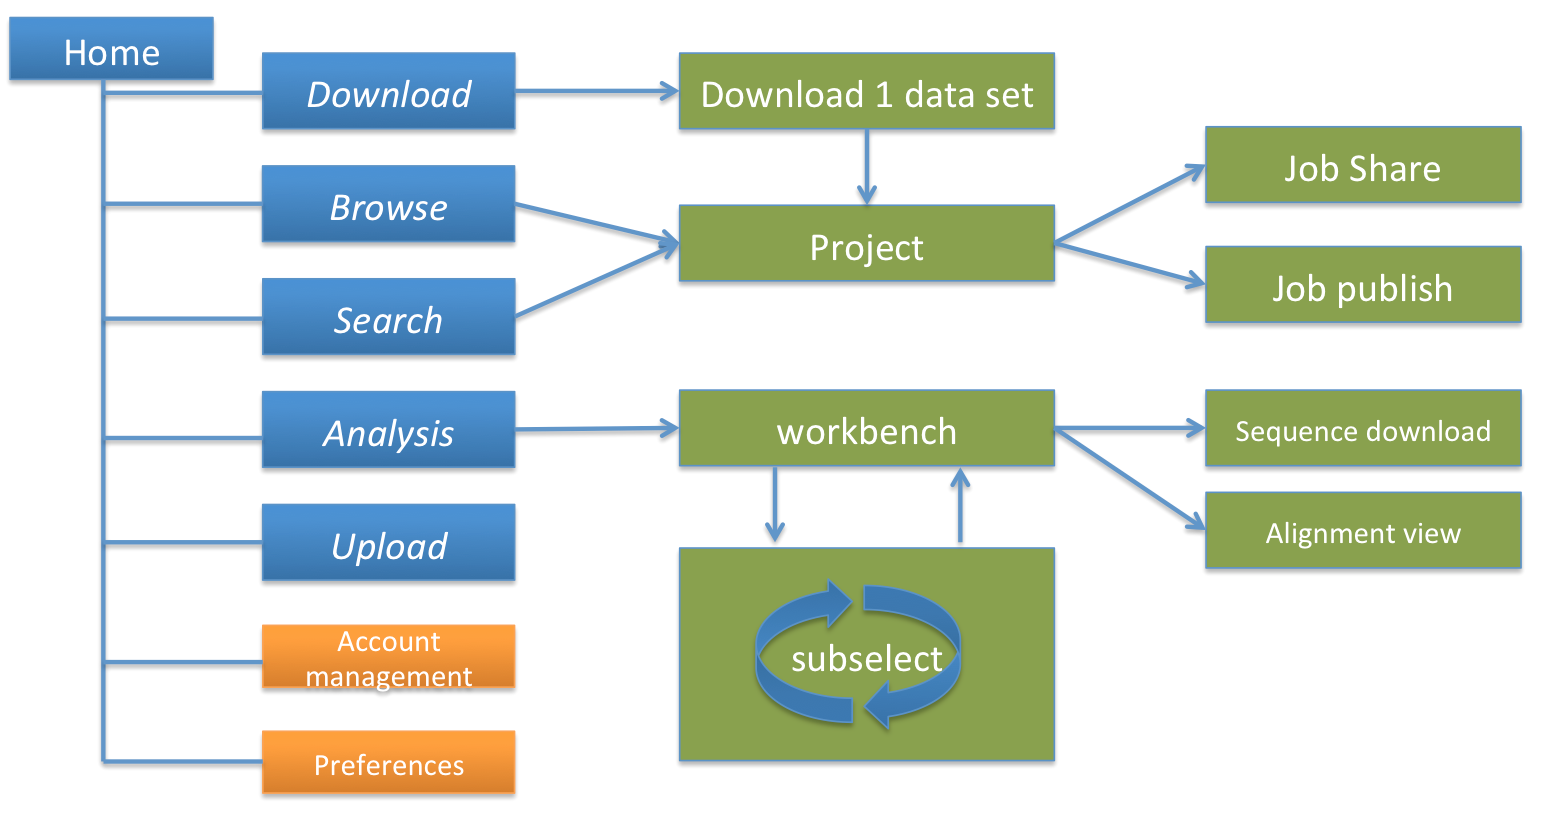
\includegraphics[width=6in]{Images/sitemap.png}
\end{center}
\caption{
Sitemap for the MG-RAST version 3 web site. On the site map the main pages are shown in blue, management pages in orange. The green boxes represent pages that are not directly accessible from the home page.
}
\label{fig:sitemap}
\end{figure*}

We note that if you want to create links to the MG-RAST web site, you should use the \textit{linkin} mechanism instead of linking to any web page directly. All pages intended for users to create external links provide the linkin feature, See Section \ref{section:linkin}.
% %%%%%%%%%%%%%%%%%%%%%%%%%%%%%%%%%%%%%%%%%%%%%%%%%%%%%%%%%%%%%%%%%%%%%%
% %%%%%%%%%%%%%%%%%%%%%%%%%%%%%%%%%%%%%%%%%%%%%%%%%%%%%%%%%%%%%%%%%%%%%%
% %%%%%%%%%%%%%%%%%%%%%%%%%%%%%%%%%%%%%%%%%%%%%%%%%%%%%%%%%%%%%%%%%%%%%%
\section{Navigation}
\label{section:website-navigation}

\begin{figure*}[ht]
\begin{center}
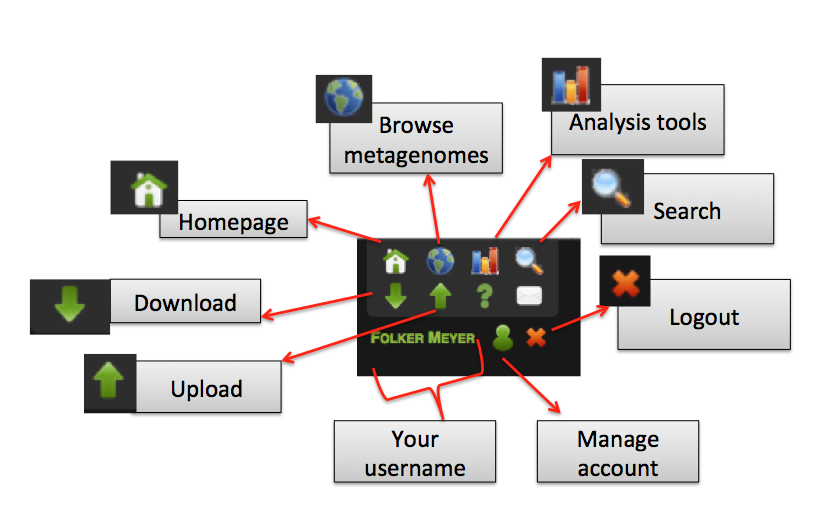
\includegraphics[width=6in]{Images/website-navigation-toolbox.png}
\end{center}
\caption{
The navigation toolbox located in the upper right hand corner of every MG-RAST web page allows easy navigation in the system.
}
\label{fig:website-navigation-toolbox}
\end{figure*}

The navigation toolkit provides easy access to the web pages listed in Section \ref{section:sitemap}. In addition, there are links to:
\begin{itemize}
\item the Account Management page -- change your name, password, email address, and manage personal preferences,

\item the Contact Page -- get in touch with the MG-RAST team, and

\item the MG-RAST blog site.
\end{itemize}
% %%%%%%%%%%%%%%%%%%%%%%%%%%%%%%%%%%%%%%%%%%%%%%%%%%%%%%%%%%%%%%%%%%%%%%
% %%%%%%%%%%%%%%%%%%%%%%%%%%%%%%%%%%%%%%%%%%%%%%%%%%%%%%%%%%%%%%%%%%%%%%
% %%%%%%%%%%%%%%%%%%%%%%%%%%%%%%%%%%%%%%%%%%%%%%%%%%%%%%%%%%%%%%%%%%%%%%
\section{Upload page}

Data and metadata can be uploaded in the form of spreadsheets along with the sequence data by using both the ftp and the http protocols. The web uploader will automatically split larger files and allow parallel uploads.

MG-RAST supports datasets that are augmented with rich metadata using the standards and technology developed by the GSC.
Each user has a temporary storage location inside the MG-RAST system. This inbox provides temporary storage for data and metadata to be submitted to the system. Using the inbox, users can extract compressed files, convert a number of vendor specific formats to MG-RAST submission-compliant formats, join paired-end reads, and obtain an \gls{MD5} checksum for verifying that transmission to MG-RAST has not altered the data.

The web uploader has been optimized for large datasets of over 100 gigabasepairs, often resulting in file sizes in excess of 150 GB.
% %%%%%%%%%%%%%%%%%%%%%%%%%%%%%%%%%%%%%%%%%%%%%%%%%%%%%%%%%%%%%%%%%%%%%%
% %%%%%%%%%%%%%%%%%%%%%%%%%%%%%%%%%%%%%%%%%%%%%%%%%%%%%%%%%%%%%%%%%%%%%%
% %%%%%%%%%%%%%%%%%%%%%%%%%%%%%%%%%%%%%%%%%%%%%%%%%%%%%%%%%%%%%%%%%%%%%%
\section{Browse page -- Metadata-enabled data discovery}

The Browse page lists all datasets visible to the user\footnote{Datasets in MG-RAST are private by default, but the submitting user has the option of sharing datasets with specific users or  making datasets public.}. This page also provides an overview of the nonpublic datasets submitted by the user or shared with the user.

Figure \ref{fig:metagenome-browser} shows the interactive metagenome browse table, which provides an interactive graphical means to discover data based on technical data (e.g., sequence type or dataset size) or metadata (e.g., location or biome).

\begin{figure*}
\begin{center}
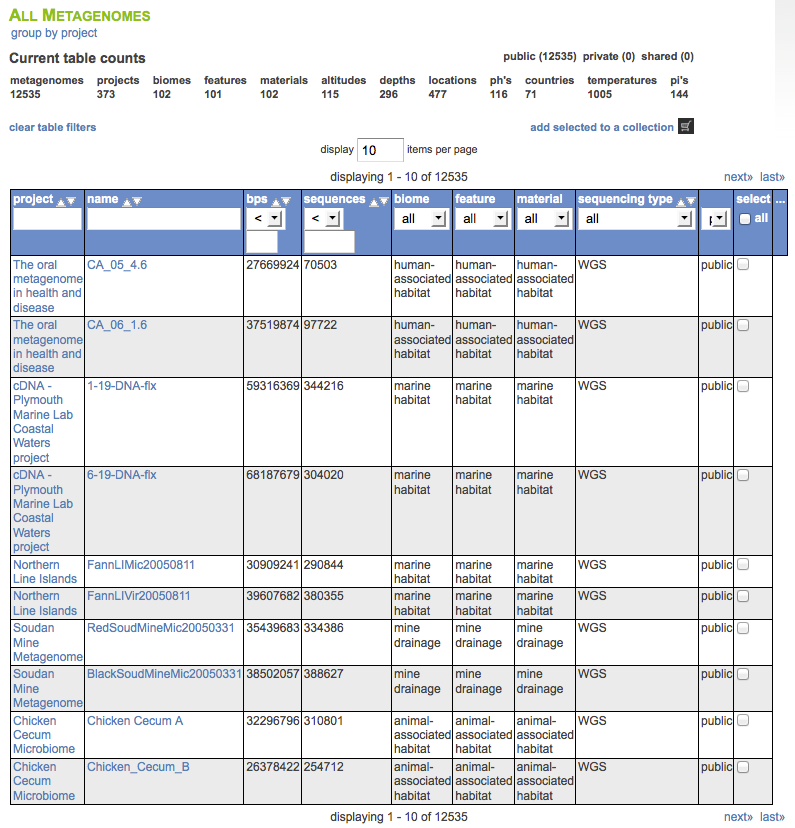
\includegraphics[width=6in]{Images/metagenome-browser.png}
\end{center}
\caption{
Browse page, enabling sorting and data search. Users can select the metadata they wish to view and search. Some of the metadata is hidden by default and can be viewed by clicking on the last column header on the right side of the table and selecting the desired columns; this can also be used to hide unwanted columns.
}
\label{fig:metagenome-browser}
\end{figure*}
% %%%%%%%%%%%%%%%%%%%%%%%%%%%%%%%%%%%%%%%%%%%%%%%%%%%%%%%%%%%%%%%%%%%%%%
% %%%%%%%%%%%%%%%%%%%%%%%%%%%%%%%%%%%%%%%%%%%%%%%%%%%%%%%%%%%%%%%%%%%%%%
% %%%%%%%%%%%%%%%%%%%%%%%%%%%%%%%%%%%%%%%%%%%%%%%%%%%%%%%%%%%%%%%%%%%%%%
\section{Project page}
Shown in Figure \ref{fig:project-page}, the project page provides a list of datasets and metadata for a project.
The table at the bottom of the Project page provides access to the individual metagenomes by clicking on the identifiers in the first column. In addition, the final column provides downloads for metadata, submitted data, and the analysis results via the three labelled arrows.

\begin{figure*}
\begin{center}
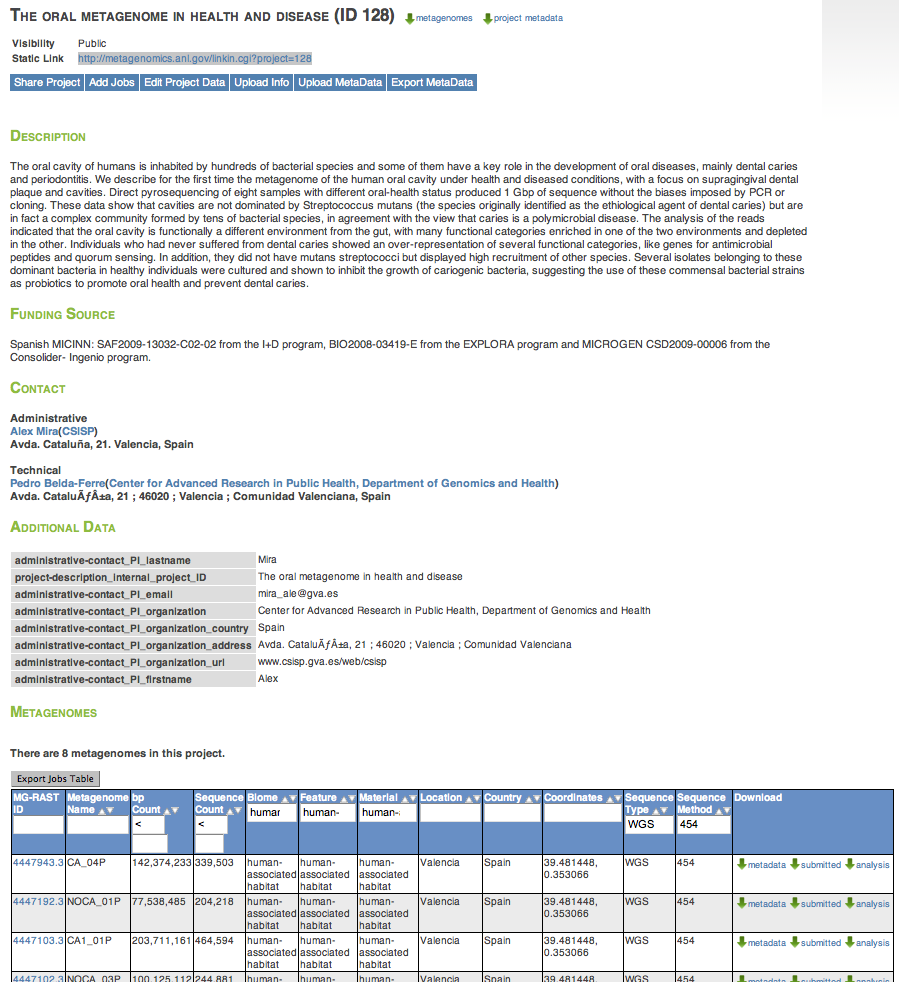
\includegraphics[width=6in]{Images/project-page.png}
\end{center}
\caption{
Project page, providing a summary of all the datasets in the project and an interface for downloads.
}
\label{fig:project-page}
\end{figure*}

For the dataset owners the Project page provides an editing capability using a number of menu entries at the top of the page. Figure \ref{fig:project-page-editing-buttons} shows the available options.

\begin{itemize}
\item Share Project --
make the data in this project available to third parties via sending them access tokens. This also allows users to grant anonymous access to manuscript reviewers for projects which have not yet been made public.

\item Add Jobs --
add additional datasets to this project.

\item Edit Project Data --
edit the contents of this page.

\item Upload Info --
upload information to be displayed on this page.

\item Upload MetaData --
upload a metadata spreadsheet for the project.

\item Export MetaData\footnote{This option is available to non-dataset owners.} --
export the metadata spreadsheet for this project.

\end{itemize}

\begin{figure*}
\begin{center}

\includegraphics[width=6in]{Images/project-page-editing-buttons.png}
\end{center}
\caption{
Buttons displayed by Project page to
dataset owner.}
\label{fig:project-page-editing-buttons}
\end{figure*}
% %%%%%%%%%%%%%%%%%%%%%%%%%%%%%%%%%%%%%%%%%%%%%%%%%%%%%%%%%%%%%%%%%%%%%%
% %%%%%%%%%%%%%%%%%%%%%%%%%%%%%%%%%%%%%%%%%%%%%%%%%%%%%%%%%%%%%%%%%%%%%%
% %%%%%%%%%%%%%%%%%%%%%%%%%%%%%%%%%%%%%%%%%%%%%%%%%%%%%%%%%%%%%%%%%%%%%%
\section{Overview page}

MG-RAST automatically creates an individual summary page for each dataset. This metagenome overview page provides a summary of the annotations for a single dataset. The page is made available by the automated pipeline once the computation is finished.
This page is a good starting point for looking at a particular dataset. It provides a significant amount of information on technical details and biological content.

The page is intended as a single point of reference for metadata, quality, and data. It also provides an initial overview of the analysis results for individual datasets with default parameters. Further analyses are available on the Analysis page.
% %%%%%%%%%%%%%%%%%%%%%%%%%%%%%%%%%%%%%%%%%%%%%%%%%%%%%%%%%%%%%%%%%%%%%%
% %%%%%%%%%%%%%%%%%%%%%%%%%%%%%%%%%%%%%%%%%%%%%%%%%%%%%%%%%%%%%%%%%%%%%%
\subsection{Technical part of the Overview page -- Details on sequencing and analysis}

The Overview page provides the MG-RAST ID for a data set, a unique identifier that is usable as accession number for publications. Additional information such as the name of the submitting PI and organization and a user-provided metagenome name are displayed at the top of the page as well. A static URL for linking to the system that will be stable across changes to the MG-RAST web interface is provided as additional information
(Figure \ref{fig:metagenome-overview}).

\begin{figure}
\begin{center}
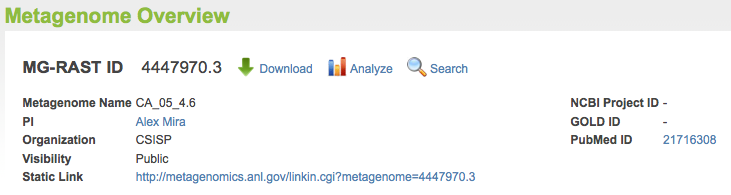
\includegraphics[width=6in]{Images/metagenome-overview.png}
\end{center}
\caption{
Top of the metagenome Overview page.
}
\label{fig:metagenome-overview}
\end{figure}

We provide an automatically generated paragraph of text describing the submitted data and the results computed by the pipeline. By means of the project information we display additional information provided by the data submitters at the time of submission or later.

One of the key diagrams in MG-RAST is the sequence breakdown pie chart (Figure \ref{fig:classification-pie-chart}) classifying the submitted sequences submitted into several categories according to their annotation status. As detailed in the description of the MG-RAST v3 pipeline above, the features annotated in MG-RAST are protein coding genes and ribosomal proteins.

\begin{figure}
\begin{center}
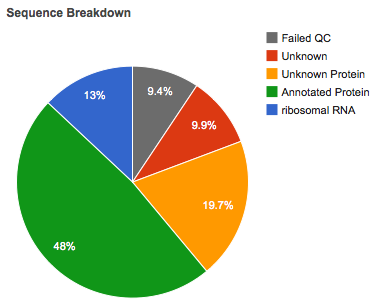
\includegraphics[width=4in]{Images/classification-pie-chart.png}
\end{center}
\caption{
Sequences to the pipeline are classified into one of five categories: grey = failed the QC, red = unknown sequences, yellow = unknown function but protein coding, green = protein coding with known function, and blue = ribosomal RNA. For this example almost 40\% of sequences were either filtered by QC or failed to be recognized as either protein coding or ribosomal.
}
\label{fig:classification-pie-chart}
\end{figure}

We note that for performance reasons no other sequence features are annotated by the default pipeline. Other feature types such as small RNAs or regulatory motifs (e.g., CRISPRs \cite{CRISPRS}) not only will require significantly higher computational resources but also are frequently not supported by the unassembled short reads that constitute the vast majority of todays metagenomic data in MG-RAST. The quality of the sequence data coming from next-generation instruments requires careful design of experiments, lest the sensitivity of the methods is greater than the signal-to-noise ratio the data supports.

The overview page also provides metadata for each dataset to the extent that such information has been made available. Metadata enables other researchers to discover datasets and compare annotations. MG-RAST requires standard metadata for data sharing and data publication. This is implemented using the standards developed by the Genomics Standards Consortium. Figure \ref{fig:GSC-MIxS-checklist-information} shows the metadata summary for a dataset.

\begin{figure}
\begin{center}
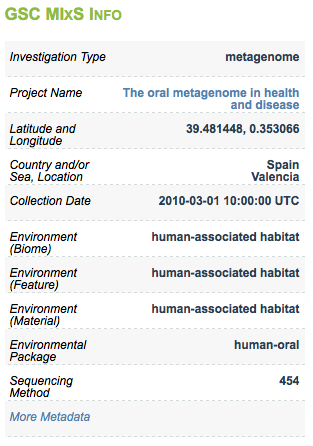
\includegraphics[width=3.5in]{Images/GSC-MIxS-checklist-information.png}
\end{center}
\caption{
Information from the GSC MIxS checklist providing minimal metadata on the sample.
}
\label{fig:GSC-MIxS-checklist-information}
\end{figure}

All metadata stored for a specific dataset is available in MG-RAST; we merely display a standardized subset in this table. A link at the bottom of the table (``More Metadata'') provides access to a table with the complete metadata. This enables users to provide extended metadata going beyond the GSC minimal standards. A mechanism to provide community consensus extensions to the minimal checklists and the environmental packages are explicitly encouraged but not required when using MG-RAST.
% %%%%%%%%%%%%%%%%%%%%%%%%%%%%%%%%%%%%%%%%%%%%%%%%%%%%%%%%%%%%%%%%%%%%%%
\subsubsection{Metagenome quality control}

The analysis flowchart and analysis statistics provide an overview of the number of sequences at each stage in the pipeline (Figure \ref{fig:analysis-flowchart}). The text block next to the analysis flowchart presents the numbers next to their definitions.
\begin{figure}
\begin{center}
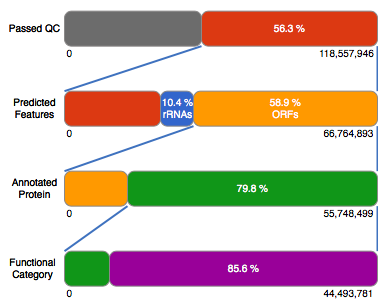
\includegraphics[width=4in]{Images/analysis-flowchart.png}
\end{center}
\caption{
Analysis flowchart providing an overview of the fractions of sequences surviving the various steps of the automated analysis. In this case about 43.7\% of sequences were filtered during quality control. From the remaining 66,764,893 sequences, 58.9\% were predicted to be protein coding, 10.4\% hit ribosomal RNA. From the predicted proteins, 79.8\% could be annotated with a putative protein function. Of 44.5 million annotated proteins, 85.6\% have been assigned to a functional classification (\gls{SEED}, COG, eggNOG, KEGG).
}
\label{fig:analysis-flowchart}
\end{figure}

% %%%%%%%%%%%%%%%%%%%%%%%%%%%%%%%%%%%%%%%%%%%%%%%%%%%%%%%%%%%%%%%%%%%%%%%%%%%%%%%
\subsubsection{Source hits distribution}
\label{section:source-hits-distribution}
The source hits distribution shows what percentage of the predicted protein features could be annotated with similarity to a protein of known function and which database those functions were from. In addition, ribosomal RNA genes are mapped to the rRNA databases.

Figure \ref{fig:source-hits-distribution} shows the number of features in this dataset that were annotated by the different databases. These include protein databases, protein databases with functional hierarchy information, and ribosomal RNA databases.

In addition this display will print the number of records in the M5nr protein database and in the M5rna ribosomal databases. 

\begin{figure}
\begin{center}
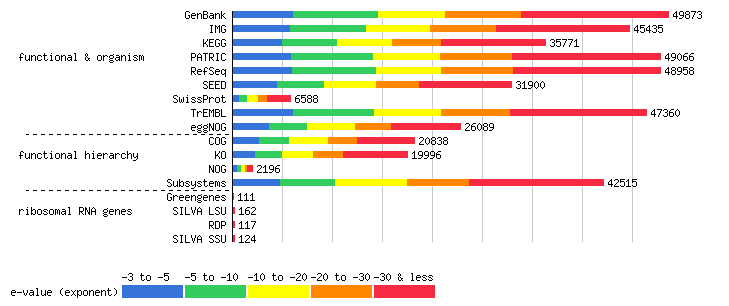
\includegraphics[width=6in]{Images/source-hits-distribution.png}
\end{center}
\caption{Graph showing the number of features in this dataset annotated by the different databases.
 The bars representing annotated reads are colored by e-value range. Different databases have different numbers of hits but can also have different types of annotation data.}
\label{fig:source-hits-distribution}
\end{figure}
% %%%%%%%%%%%%%%%%%%%%%%%%%%%%%%%%%%%%%%%%%%%%%%%%%%%%%%%%%%%%%%%%%%%%%%
\subsubsection{Other statistics }

MG-RAST also provides a quick link to other statistics.
%a general statistical overview of the different analysis steps performed (see the Analysis flowchart), a comprehensive list of all metadata for the dataset, sequence length and GC distributions.

\noindent For example, the Analysis Statistics and Analysis Flowchart provide sequence statistics for the main steps in the pipeline from raw data to annotation, describing the transformation of the data between steps.
Sequence length and GC histograms display the distribution before and after quality control steps.
Metadata is presented in a searchable table that contains contextual metadata describing sample location, acquisition, library construction, and sequencing using GSC compliant metadata. All metadata can be downloaded from the table.

In addition, 
a breakdown of BLAT hits is provided  per data source (e.g., hits to RefSeq \cite{REFSEQ}, UniProt \cite{UNIPROT}, or \gls{SEED} \cite{SUBSYSTEMS}).
%\subsection{Taxonomic and functional information on the overview page}
% %%%%%%%%%%%%%%%%%%%%%%%%%%%%%%%%%%%%%%%%%%%%%%%%%%%%%%%%%%%%%%%%%%%%%%
% %%%%%%%%%%%%%%%%%%%%%%%%%%%%%%%%%%%%%%%%%%%%%%%%%%%%%%%%%%%%%%%%%%%%%%
\subsection{Biological part of the Overview page }

The taxonomic hit distribution display divides taxonomic units into a series of pie charts of all the annotations grouped at various taxonomic ranks (domain, phylum, class, order, family, genus). The subsets are selectable for downstream analysis; this also enables downloads of subsets of reads, for example, those hitting a specific taxonomic unit.
% %%%%%%%%%%%%%%%%%%%%%%%%%%%%%%%%%%%%%%%%%%%%%%%%%%%%%%%%%%%%%%%%%%%%%%
\subsubsection{Rank abundance}

The rank abundance plot (Figure \ref{fig:rank-abundance}) provides a rank-ordered list of taxonomic units at a user-defined taxonomic level, ordered by their abundance in the annotations.

\begin{figure}
\begin{center}
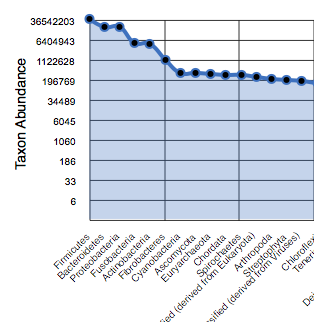
\includegraphics[width=3in]{Images/rank-abundance.png}
\end{center}
\caption{
Sample rank abundance plot by phylum.
}
\label{fig:rank-abundance}
\end{figure}
% %%%%%%%%%%%%%%%%%%%%%%%%%%%%%%%%%%%%%%%%%%%%%%%%%%%%%%%%%%%%%%%%%%%%%%
\subsubsection{Rarefaction}
The rarefaction curve of annotated species richness is a plot (see Figure \ref{fig:rarefaction} of the total number of distinct species annotations as a function of the number of sequences sampled.
The slope of the right-hand part of the curve is related to the fraction of sampled species that are rare.
On the left, a steep slope indicates that a large fraction of the species diversity remains to be discovered. If the curve becomes flatter to the right, a reasonable number of individuals is sampled: more intensive sampling is likely to yield only few additional species.
Sampling curves generally rise quickly at first and then level off toward an asymptote as fewer new species are found per unit of individuals collected.

%These rarefaction curves are calculated from the table of species abundance. The curves represent the average number of different species annotations for subsamples of the complete dataset.

\begin{figure*}
\begin{center}
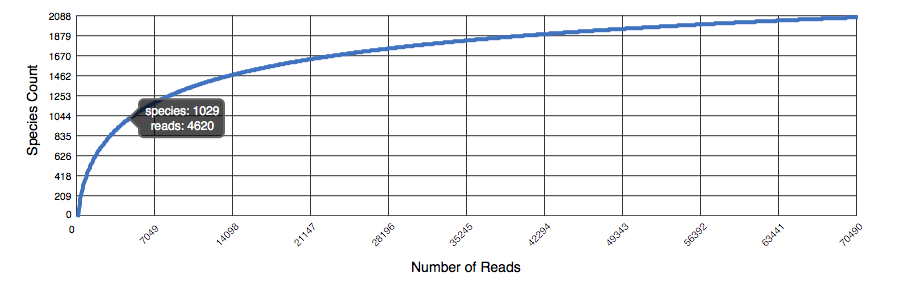
\includegraphics[width=6in]{Images/rarefaction.png}
\end{center}
\caption{
Rarefaction plot showing a curve of annotated species richness. This curve is a plot of the total number of distinct species annotations as a function of the number of sequences sampled.
}
\label{fig:rarefaction}
\end{figure*}

The rarefaction curve is derived from the protein taxonomic annotations and is subject to problems stemming from technical artifacts. These artifacts can be similar to the ones affecting amplicon sequencing \cite{RARE}, but the process of inferring species from protein similarities may introduce additional uncertainty.

% Sampling curves generally rise very quickly at first and then level off towards an asymptote a%s fewer new species are found per unit of individuals collected. These rarefaction curves are c%alculated from the table of species abundance. The curves represent the average number of di%fferent species annotations for subsamples of the the complete dataset.
% %%%%%%%%%%%%%%%%%%%%%%%%%%%%%%%%%%%%%%%%%%%%%%%%%%%%%%%%%%%%%%%%%%%%%%
\subsubsection{Alpha diversity}
In this section we display an estimate of the alpha diversity based on the taxonomic annotations for the predicted proteins. The alpha diversity is presented in context of other metagenomes in the same project (see Figure \ref{fig:alpha-diversity}).

\begin{figure*}
\begin{center}
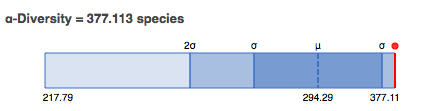
\includegraphics[width=6in]{Images/alpha-diversity.png}
\end{center}
\caption{
Alpha diversity plot showing the range of  {$\alpha$}-diversity values in the project the data set belongs to. The min, max, and mean values are shown, with the standard deviation ranges ($\sigma$ and $2\sigma$) in different shades. The {$\alpha$}-diversity of this metagenome is shown in red.
}
\label{fig:alpha-diversity}
\end{figure*}

The alpha diversity estimate is a single number that summarizes the distribution of species-level annotations in a dataset.   The Shannon diversity index is an abundance-weighted average of the logarithm of the relative abundances of annotated species.

We compute the species richness as the antilog of the Shannon diversity:

$$ \textrm{Richness} = 10^{-\sum_i  p_i \log(p_i) }  $$

\noindent
where $p_i$ are the proportions of annotations in each of the species categories.
Shannon species richness
%is the antilog of the Shannon index
has units of  the ``effective number of species''. Each $p$ is a ratio of the number of annotations for each species to the total number of annotations.
%and m is the total number of different species annotations.
The species-level annotations are from all the annotation source databases used by MG-RAST. The table of species and number of observations used to calculate this diversity estimate can be downloaded under ``download source data'' on the Overview page.
% %%%%%%%%%%%%%%%%%%%%%%%%%%%%%%%%%%%%%%%%%%%%%%%%%%%%%%%%%%%%%%%%%%%%%%
\subsubsection{Functional categories}

This section contains four pie charts providing a breakdown of the functional categories for KEGG \cite{KEGG}, COG \cite{COG}, \gls{SEED} \gls{Subsystem}s \cite{SUBSYSTEMS}, and eggNOGs \cite{EGGNOG}. Clicking on the individual pie chart slices will save the respective sequences to the workbench.
The relative abundance of sequences per functional category can be downloaded as a spreadsheet, and users can browse the functional breakdowns via the Krona tool \cite{KRONA} integrated in the page.

A more detailed functional analysis, allowing the user to manipulate parameters for sequence similarity matches, is available from the Analysis page.

\begin{figure*}
\begin{center}
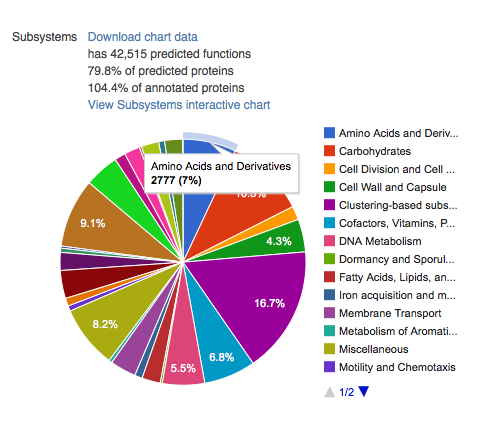
\includegraphics[width=6in]{Images/subsystems-functions-piechart.png}
\end{center}
\caption{
The \gls{Subsystem}s function piechart, showing reads classified into SEED subsystem level-one functions. In contrast to the COG, eggNOG, and KEGG classification schemes, there are over 20 top-level subsystem categories, creating a more highly resolved ``fingerprint" for the metagenome.
}
\label{fig:subsystems-functions-piechart}
\end{figure*}

%\textbf{QUESTION:: What are the default parameters used to display these graphs??} BEST HIT REP HIT?

% %%%%%%%%%%%%%%%%%%%%%%%%%%%%%%%%%%%%%%%%%%%%%%%%%%%%%%%%%%%%%%%%%%%%%%
%\subsubsection{Taxonomic breakdown}

%This section contains 6 pie charts representing the break

% %%%%%%%%%%%%%%%%%%%%%%%%%%%%%%%%%%%%%%%%%%%%%%%%%%%%%%%%%%%%%%%%%%%%%%
% %%%%%%%%%%%%%%%%%%%%%%%%%%%%%%%%%%%%%%%%%%%%%%%%%%%%%%%%%%%%%%%%%%%%%%
\section{Download page}

The Download page provides all publicly available datasets for download.
Three types of data are available for download.

\begin{itemize}
\item Metadata --
data describing data in GSC-compliant format.

\item Submitted data --
the original user submission.

\item Analysis results --
results of running the MG-RAST pipeline. The list includes all intermediate data products and is intended to serve as a basis for further analysis outside the MG-RAST pipeline.

Details on the individual files are in Appendix \ref{chapter:downloads}.
\end{itemize}
% %%%%%%%%%%%%%%%%%%%%%%%%%%%%%%%%%%%%%%%%%%%%%%%%%%%%%%%%%%%%%%%%%%%%%%
% %%%%%%%%%%%%%%%%%%%%%%%%%%%%%%%%%%%%%%%%%%%%%%%%%%%%%%%%%%%%%%%%%%%%%%
% %%%%%%%%%%%%%%%%%%%%%%%%%%%%%%%%%%%%%%%%%%%%%%%%%%%%%%%%%%%%%%%%%%%%%%
\section{Search Page}
\label{section:search-page}

In addition to the Browse page, one can use
the Search page to find datasets in MG-RAST.
The basic function of the Search page is to find data sets that (1) contain a search string in the metadata (dataset name, project name, project description, GSC metadata), (2) contain specific functions (e.g., SEED functional roles, SEED subsystems, or GenBank annotations), or (3) contain specific organisms. The default search uses all three kinds of data.

In addition to a Google-like search that searches all data fields, we provide specialized searches in one of the three data types. Figure
\ref{fig:search-page-unsorted-results} shows the result of a metadata search for ``oral health.''
Figure \ref{fig:search-page-sorted-results} shows the results from Figure \ref{fig:search-page-unsorted-results} after sorting by metagenome ID.

\begin{figure}
\begin{center}
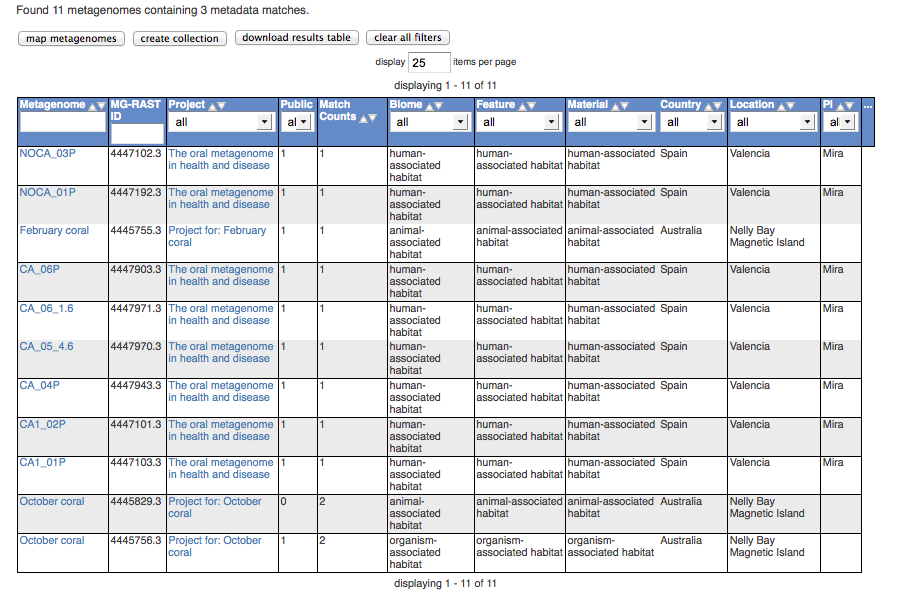
\includegraphics[width=6in]{Images/search-page-unsorted-results.png}
\end{center}
\caption{Searching for ``oral health" returns 11 data sets for two projects. }
\label{fig:search-page-unsorted-results}
\end{figure}

\begin{figure}
\begin{center}
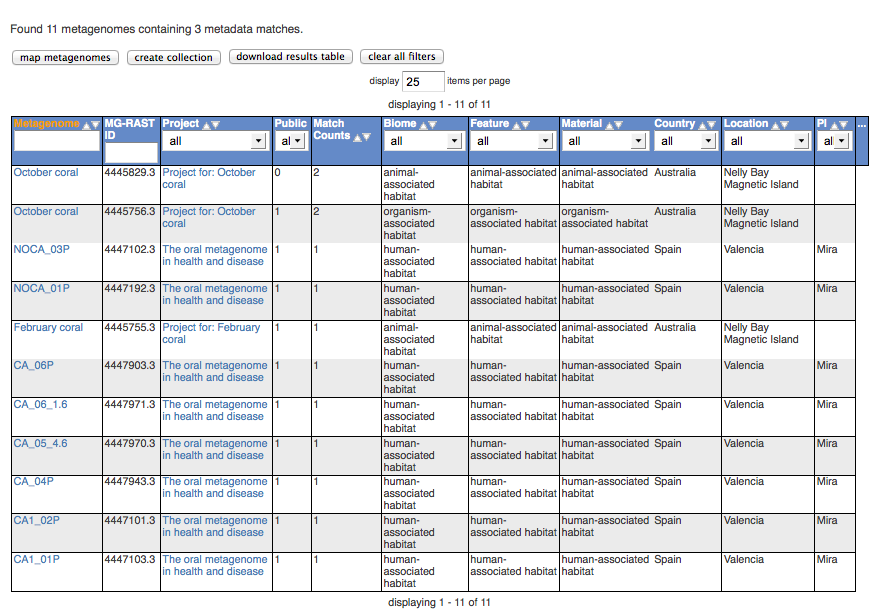
\includegraphics[width=6in]{Images/search-page-sorted-results.png}
\end{center}
\caption{Search results from the previous search sorted by projects.}
\label{fig:search-page-sorted-results}
\end{figure}
% %%%%%%%%%%%%%%%%%%%%%%%%%%%%%%%%%%%%%%%%%%%%%%%%%%%%%%%%%%%%%%%%%%%%%%
% %%%%%%%%%%%%%%%%%%%%%%%%%%%%%%%%%%%%%%%%%%%%%%%%%%%%%%%%%%%%%%%%%%%%%%
% %%%%%%%%%%%%%%%%%%%%%%%%%%%%%%%%%%%%%%%%%%%%%%%%%%%%%%%%%%%%%%%%%%%%%%
\section{Analysis page}
\label{section:analysis-page}

The MG-RAST annotation pipeline produces a set of annotations for each sample; these annotations can be interpreted as functional or taxonomic abundance profiles. The analysis page can be used to view these profiles for a single metagenome or to compare profiles from multiple metagenomes using various visualizations (e.g., heatmap) and statistics (e.g., PCoA, normalization).

The page is divided into three parts following a typical workflow (Figure \ref{fig:analysis-page}).

\begin{figure*}
\begin{center}
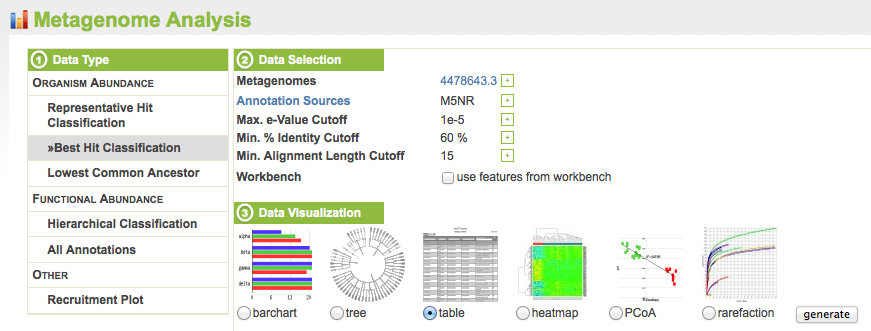
\includegraphics[width=6in]{Images/analysis-page.png}
\end{center}
\caption{
Three-step process in using the Analysis page: (1) select a profile and hit (see text) type; (2) select a list of metagenomes and set annotation source and similarity parameters; (3) choose a comparison.
}
\label{fig:analysis-page}
\end{figure*}
\begin{enumerate}

\item \textbf{Data type}

Selection of an MG-RAST analysis scheme, that is, selection of a particular taxonomic or functional abundance profile mapping. For taxonomic annotations, since there is not always a unique mapping from hit to annotation, we provide three interpretations: best hit, representative hit, and lowest common ancestor (LCA), as explained in Section \ref{section:hit-types}.

We note that when choosing the LCA annotations, not all downstream tools are available. The reason is that for the LCA annotations not all sequences will be annotated to the same level: classifications are returned on different taxonomic levels.

Functional annotations can be grouped into mappings to functional hierarchies or can be displayed without a hierarchy. In addition, the recruitment plot displays the recruitment of protein sequences against a reference genome.

Each selected data type has data selections and data visualizations specific for it.

\item \textbf{Data selection}

Selection of sample and parameters. This dialog allows the selection of multiple metagenomes that can be compared individually or selected and compared as groups. Comparison is always relative to the annotation source, e-value, and percent identity cutoffs selectable in this section. In addition to the metagenomes available in MG-RAST, sets of sequences previously saved in the workbench can be selected for visualization.

\item \textbf{Data visualization}

Data visualization and comparison. Depending on the selected profile type, the profiles for the metagenomes can be visualized and compared using barcharts, trees, spreadsheet-like tables, heatmaps, PCoA, rarefaction plots, circular recruitment plot, and KEGG maps.
\end{enumerate}

%The analysis page offers several hit classification schemes that are explained in Section \ref{section:hit-types}.

The data selection dialogue provides access to data sets in four ways. The four categories can be selected from a pulldown menu.

\begin{itemize}
\item \textbf{private} data --
list of private or shared data sets for browsing under ``available metagenomes''.

\item \textbf{collections} --
defined sets of metagenomes grouped for easier analysis. This is the recommended way of working with the analysis page.

\item \textbf{projects} --
global groups of datasets grouped by the submitting user. The project name will be displayed.

\item \textbf{public} data --
display of all public datasets.

\end{itemize}

When using collections or projects, data can also be grouped into one set per collection or project and subsequently compared or added.

\begin{figure*}
\begin{center}
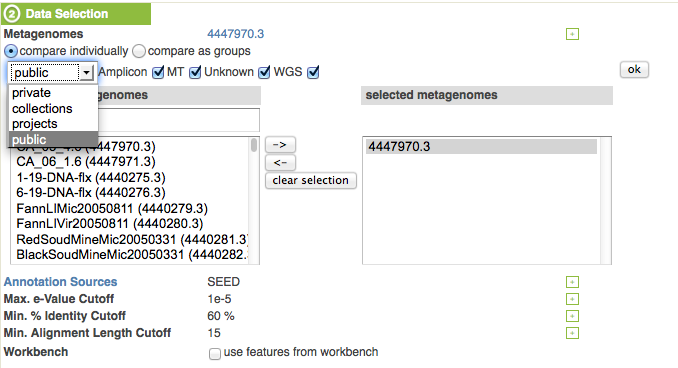
\includegraphics[width=6in]{Images/Data-selection-expanded.png}
\end{center}
\caption{
View of the data selection dialogue, with the list of four data categories expanded.
}
\label{fig:Data-selection-expanded}
\end{figure*}

Once a category is selected, the data browser underneath ``available metagenomes'' will display data of the selected category. The text field under ``available metagenomes'' displays the available datasets or group identifiers.

The use of MG-RAST identifiers (e.g., 4447971.3) is possible in the text field underneath ``available metagenomes.''
% %%%%%%%%%%%%%%%%%%%%%%%%%%%%%%%%%%%%%%%%%%%%%%%%%%%%%%%%%%%%%%%%%%%%%%
% %%%%%%%%%%%%%%%%%%%%%%%%%%%%%%%%%%%%%%%%%%%%%%%%%%%%%%%%%%%%%%%%%%%%%%
% %%%%%%%%%%%%%%%%%%%%%%%%%%%%%%%%%%%%%%%%%%%%%%%%%%%%%%%%%%%%%%%%%%%%%%
\subsection{Normalization}

Normalization refers to a transformation that attempts to reshape an underlying distribution. A large number of biological variables exhibit a log-normal distribution, meaning that when the data is transformed with a log transformation, the values exhibit a normal distribution. Log transformation of the counts data makes a normalized data product that is more likely to satisfy the assumptions  of additional downstream tests such as ANOVA or t-tests.

Standardization is a transformation applied to each distribution in a group of distributions so that all distributions exhibit the same mean and the same standard deviation. This removes some aspects of intersample variability and can make data more comparable. This sort of procedure is analogous to commonly practiced scaling procedures but is more robust in that it controls for both scale and location.

The Analysis page calculates the ordination visualizations with either raw or normalized counts, at the user's option. The normalization procedure is
as follows.

\begin{small}
\begin{math}
normalized\_value\_i = log2(raw\_counts\_i + 1)
\end{math}
\end{small}

\noindent
The standardized values then are calculated from the normalized values by subtracting the mean of each sample's normalized values and dividing by the standard deviation of each sample's normalized values.

\begin{small}
\begin{math}
standardized\_i = (normalized\_i - mean(normalized\_i)) / stddev(normalized\_i)
\end{math}
\end{small}

More about these procedures is available in a number of texts. We recommend Terry Speed's ``Statistical Analysis of Gene Expression in Microarray Data" \cite{1584883278}.

When data exhibit a nonnormal, normal, or unknown distribution, nonparametric tests (e.g., Man-Whitney or Kurskal-Wallis) should be used. Boxplots are easy to use, and the MG-RAST analysis page provides boxplots of the standardized abundance values for checking the comparability of samples (Figure \ref{fig:boxplots}).

\begin{figure}
\begin{center}
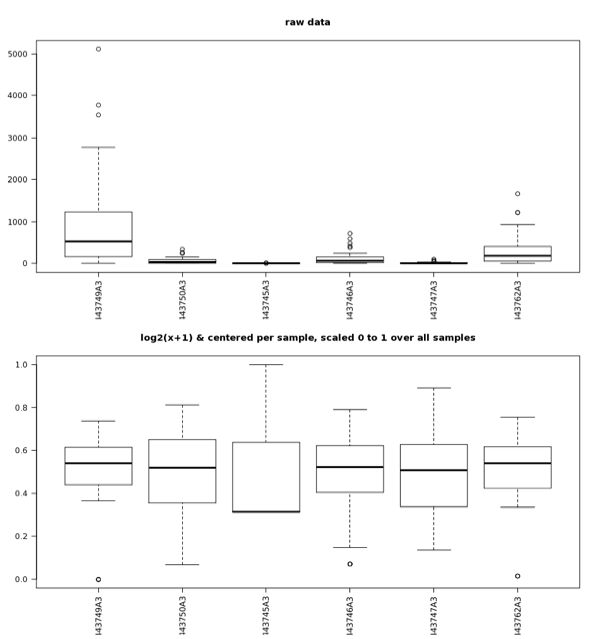
\includegraphics[width=3in]{Images/boxplots.png}
\end{center}
\caption{
Boxplots of the abundance data for raw values (top) as well as values that have undergone the normalization and standardization procedures (bottom) described in the text. After normalization and standardization, samples exhibit value distributions that are much more comparable and that have a normal distribution; the normalized and standardized data are suitable for analysis with parametric tests; the raw data are not.
}
\label{fig:boxplots}
\end{figure}
% %%%%%%%%%%%%%%%%%%%%%%%%%%%%%%%%%%%%%%%%%%%%%%%%%%%%%%%%%%%%%%%%%%%%%%
% %%%%%%%%%%%%%%%%%%%%%%%%%%%%%%%%%%%%%%%%%%%%%%%%%%%%%%%%%%%%%%%%%%%%%%
\subsection{Rarefaction}
\label{section:analysis-page-rarefaction}

The rarefaction view is available only for taxonomic data. The
rarefaction curve of annotated species richness is a plot (see Figure
\ref{fig:analysis-page-rarefaction-example}) of the total number
of distinct species annotations as a function of the number of
sequences sampled. As shown in Figure \ref{fig:analysis-page-rarefaction-example},
multiple data sets can be included.

The slope of the right-hand part of the curve is related to the fraction of sampled species that are rare. When the rarefaction curve is flat, more intensive sampling is likely to yield only a few additional species. The rarefaction curve is derived from the protein taxonomic annotations and is subject to problems stemming from technical artifacts. These artifacts can be similar to the ones affecting amplicon sequencing \cite{RARE}, but the process of inferring species from protein similarities may introduce additional uncertainty.

On the Analysis page the rarefaction plot serves as a means of comparing species richness between samples in a way independent of the sampling depth.

\begin{figure*}
\begin{center}
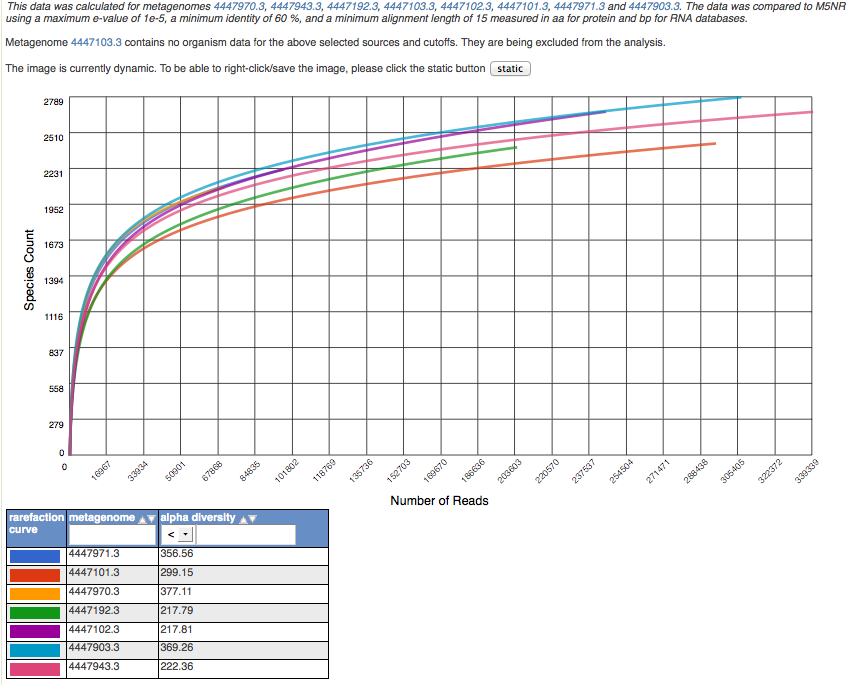
\includegraphics[width=6in]{Images/analysis-page-rarefaction-example.png}
\end{center}
\caption{
Rarefaction plot showing a curve of annotated species richness. This curve is a plot of the total number of distinct species annotations as a function of the number of sequences sampled.
}
\label{fig:analysis-page-rarefaction-example}
\end{figure*}

On the left, a steep slope indicates that a large fraction of the species diversity remains to be discovered. If the curve becomes flatter to the right, a reasonable number of individuals is sampled: more intensive sampling is likely to yield only a few additional species.

Sampling curves generally rise very quickly at first and then level off toward an asymptote as fewer new species are found per unit of individuals collected. These rarefaction curves are calculated from the table of species abundance. The curves represent the average number of different species annotations for subsamples of the the complete dataset.


%GWP: important - this repeats word for word (but with different image) the material on p. 41 under 3.6.2.2

% %%%%%%%%%%%%%%%%%%%%%%%%%%%%%%%%%%%%%%%%%%%%%%%%%%%%%%%%%%%%%%%%%%%%%%
% %%%%%%%%%%%%%%%%%%%%%%%%%%%%%%%%%%%%%%%%%%%%%%%%%%%%%%%%%%%%%%%%%%%%%%
\subsection{KEGG mapper}
\label{section:kegg-mapper}
%It provides the ability to compare datasets visually on the basis of their mapping onto a KEGG pathway map.

The KEGG map tool allows the visual comparison of predicted metabolic pathways in metagenomic samples.
It maps the abundance of identified enzymes onto a KEGG \cite{KEGG} map of functional pathways; note that the mapper is available only for functional data).
Users can select from any available KEGG pathway map.
Different colors indicate different metagenomic datasets.

The KEGG mapper works by providing two buffers that users can assign datasets to.
After loading the buffers with the intended datasets, the KEGG mapper can highlight parts of the KEGG map that are present in the dataset.
Several combinations of the two datasets can be displayed, as shown in Figure \ref{fig:analysis-page-kegg-mapper-options}.
Metagenomes can be assigned into one of two groups, and those groups can be visually compared
(see Figure \ref{fig:analysis-page-kegg-mapper-example}).

\begin{figure}
\begin{center}
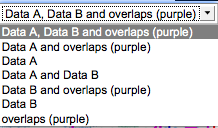
\includegraphics[width=2in]{Images/analysis-page-kegg-mapper-options.png}
\end{center}
\caption{Options available for coloring the KEGG maps.}
\label{fig:analysis-page-kegg-mapper-options}
\end{figure}

\begin{figure}[ht]
\begin{center}
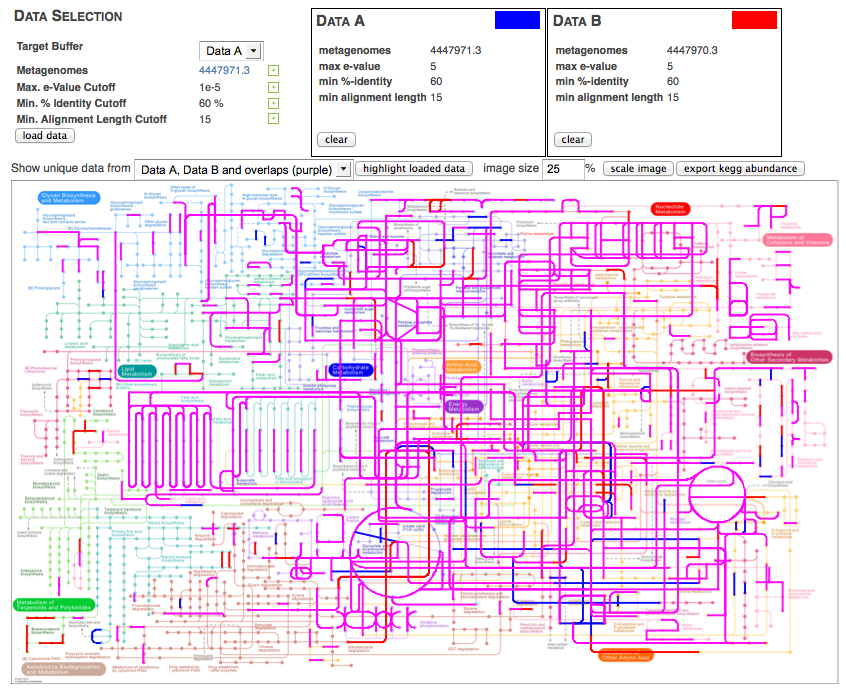
\includegraphics[width=6in]{Images/analysis-page-kegg-mapper-example.png}
\end{center}
\caption{Comparison of two datasets using the KEGG mapper. Parts of metabolism common are shown in purple; unique to A are in blue; unique to B are in red.}
\label{fig:analysis-page-kegg-mapper-example}
\end{figure}
% %%%%%%%%%%%%%%%%%%%%%%%%%%%%%%%%%%%%%%%%%%%%%%%%%%%%%%%%%%%%%%%%%%%%%%
% %%%%%%%%%%%%%%%%%%%%%%%%%%%%%%%%%%%%%%%%%%%%%%%%%%%%%%%%%%%%%%%%%%%%%%
\subsection{Recruitment plots}
\label{section:recruitment-plots}

The recruitment page allows mapping of protein sequences in a single metagenome onto the complete genome sequences that are represented in the M5nr.
Once the metagenome is selected, the page will provide a list of genomes, sorted by the number of hits per genome, from which the user can choose a genome to display (see Figure \ref{fig:analysis-page-recruitment-plot-genome-selection}).

\begin{figure}
\begin{center}
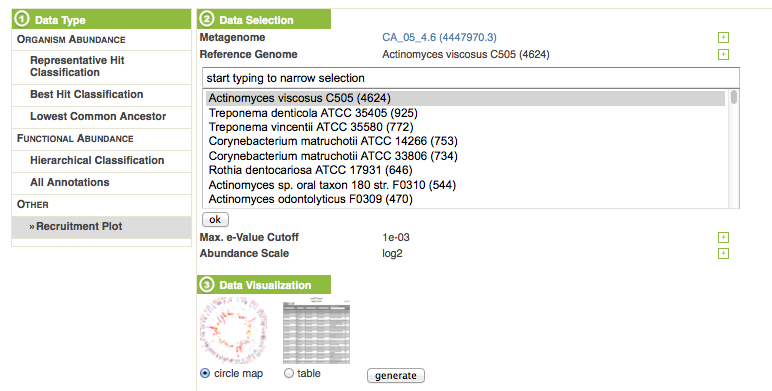
\includegraphics[width=6in]{Images/analysis-page-recruitment-plot-genome-selection.png}
\end{center}
\caption{
Selection of a genome for display, sorted by number of hits per genome.
}
\label{fig:analysis-page-recruitment-plot-genome-selection}
\end{figure}

A circular genome plot or a table will be printed. See Figure \ref{fig:analysis-page-recruitment-plot-example}
for an example. The following elements are contained in the figure:

\begin{itemize}
\item outmost circle: forward strand genes (red: protein, black: RNA)
\item 2nd circle: contigs for the reference genome
\item 3rd circle: reverse strand genes (red: protein, black: RNA)
\item innermost circle: abundance information (color coded for e-value)
\end{itemize}

\begin{figure}
\begin{center}
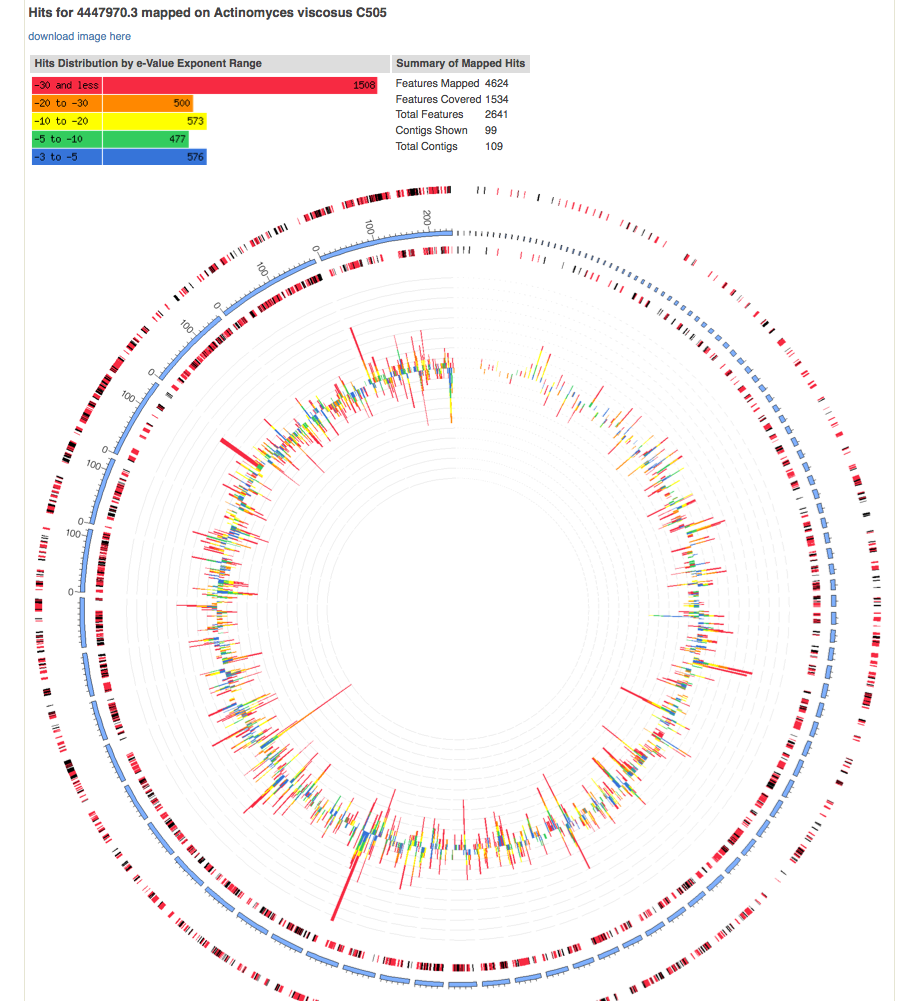
\includegraphics[width=6in]{Images/analysis-page-recruitment-plot-example.png}
\end{center}
\caption{
Example recruitment plot with the parameters from the previous figure for \textit{Actinomyces viscosus} C505.
}
\label{fig:analysis-page-recruitment-plot-example}
\end{figure}

The table view has the same information as the circular view and can easily be downloaded into a local spreadsheet. We use RefSeq\cite{REFSEQ} identifiers for the table as well as RefSeq functions because the underlying contig information is present in the GenBank\cite{GENBANK} downloads.

The recruitment plot uses the best hit approach.
% %%%%%%%%%%%%%%%%%%%%%%%%%%%%%%%%%%%%%%%%%%%%%%%%%%%%%%%%%%%%%%%%%%%%%%
% %%%%%%%%%%%%%%%%%%%%%%%%%%%%%%%%%%%%%%%%%%%%%%%%%%%%%%%%%%%%%%%%%%%%%%
\subsection{Bar charts}
\label{section:bar-charts}

\begin{figure}
\begin{center}
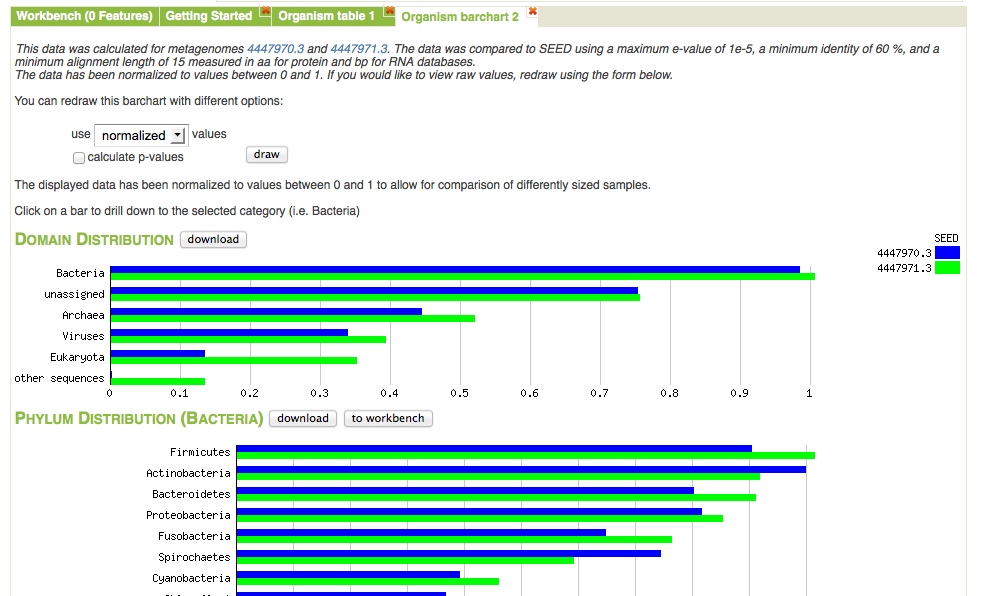
\includegraphics[width=6in]{Images/analysis-page-bar-chart.png}
\end{center}
\caption{
Bar chart view comparing normalized abundance of taxa. We have expanded the Bacteria domain to display the next level of the hierarchy.
}
\label{fig:analysis-page-bar-chart}
\end{figure}

Figure \ref{fig:analysis-page-bar-chart} shows the bar chart visualization option on the Analysis page. One important property of the page is the built-in ability to drill down by clicking on a specific category. In this example we have expanded the domain Bacteria to show the normalized abundance (adjusted for sample sizes) of bacterial phyla. The abundance information displayed can be downloaded into a local spreadsheet. Once a subselection has been made (e.g., the domain Bacteria selected), data can be sent to the workbench for detailed analysis.
%The barchart and tree tools map raw or normalized abundances onto functional or taxonomic hierarchies.
%The barchart tool presents mapping onto the highest category of a hierarchy (e.g. Domain) and allows a drill down into the hierarchy.
In addition, reads from a specific level can be added into the workbench.
% %%%%%%%%%%%%%%%%%%%%%%%%%%%%%%%%%%%%%%%%%%%%%%%%%%%%%%%%%%%%%%%%%%%%%%
% %%%%%%%%%%%%%%%%%%%%%%%%%%%%%%%%%%%%%%%%%%%%%%%%%%%%%%%%%%%%%%%%%%%%%%
\subsection{Tree diagram}

Figure \ref{fig:analysis-page-radial-tree}
shows the tree diagram option on the Analysis page.

\begin{figure}
\begin{center}
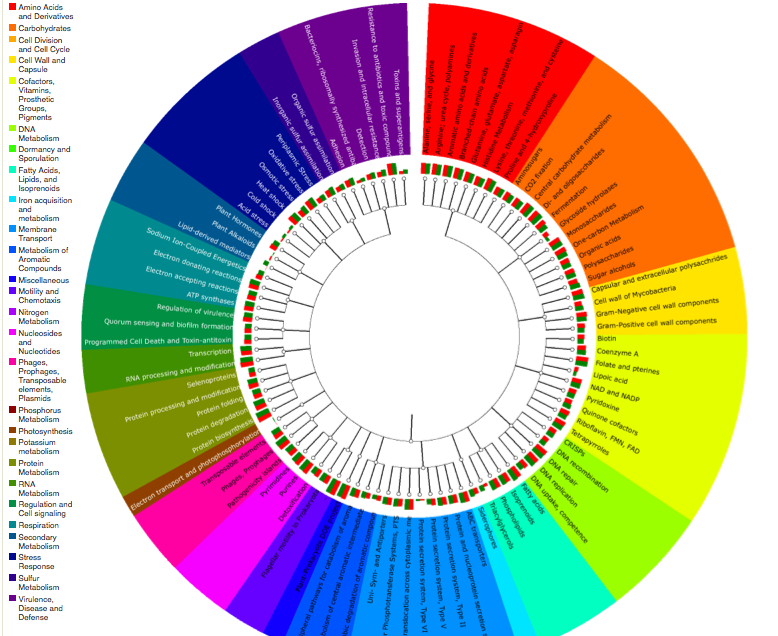
\includegraphics[width=6in]{Images/analysis-page-radial-tree.png}
\end{center}
\caption{
Tree diagram visualization option on the Analysis page.
}
\label{fig:analysis-page-radial-tree}
\end{figure}

The tree diagram allows comparison of datasets against a hierarchy (e.g., \gls{Subsystem}s or the NCBI taxonomy).
The hierarchy is displayed as a rooted tree, and the abundance (normalized for dataset size or raw) for each dataset in the various categories is displayed as a bar chart for each category.
By clicking on a category (inside the circle), detailed information can be requested for that node; see Figure \ref{fig:analysis-page-tree-additional-bar-charts}.

\begin{figure}
\begin{center}
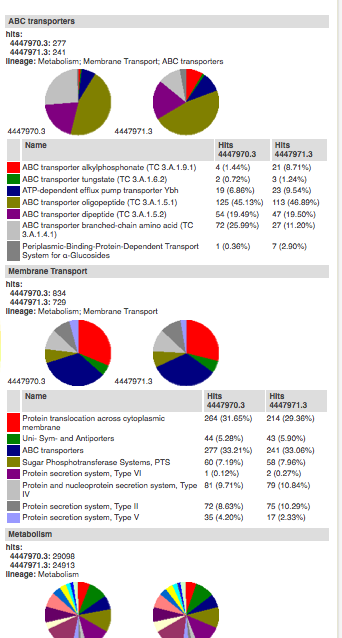
\includegraphics[width=4in]{Images/analysis-page-tree-additional-bar-charts.png}
\end{center}
\caption{
Tree diagram provision for detailed information: 
clicking on a node in the tree diagram will display addition information to the right of the tree display.
}
\label{fig:analysis-page-tree-additional-bar-charts}
\end{figure}

The tree offers several other capabilities, as shown in Figure \ref{fig:analysis-page-tree-options}.

\begin{figure}[ht]
\begin{center}
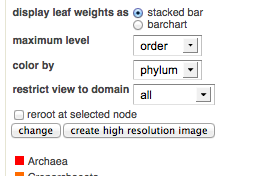
\includegraphics[width=4in]{Images/analysis-page-tree-options.png}
\end{center}
\caption{
Options for the tree view.
}
\label{fig:analysis-page-tree-options}
\end{figure}

\begin{itemize}

\item Export of a high-resolution image --
For publication purposes we provide an SVG version of the image.

\item Rerooting --
The tree display allows zooming in by rerooting the tree display. The user selects a node inside the tree (turning it red), and then selects ``reroot'' at the selected node. See Figure \ref{fig:analysis-page-tree-options}.

\item Bar chart or stacked chart --
The hierarchy entries can be displayed as bar charts per node or as a stacked graph.

\item Restrict to domain --
Is identical to rerooting the tree for a specific domain.

\item Maximum level --
This setting determines the depth of the tree being displayed.

\item Color by --
This setting determines the color (if any) used for the outer circle of the display.
\end{itemize}

Figure \ref{fig:analysis-page-tree-order-level-with-phylum-colors} shows the result of changing the display depth and coloring options. The color is used to group organisms visually into order level groups.

\begin{figure}
\begin{center}
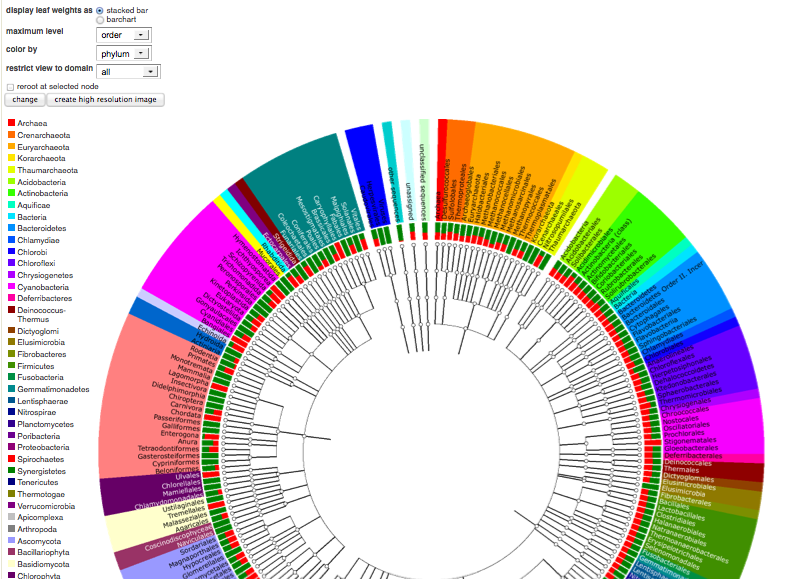
\includegraphics[width=6in]{Images/analysis-page-tree-order-level-with-phylum-colors.png}
\end{center}
\caption{
Tree view at order level with coloring set to phylum level.
}
\label{fig:analysis-page-tree-order-level-with-phylum-colors}
\end{figure}

% %%%%%%%%%%%%%%%%%%%%%%%%%%%%%%%%%%%%%%%%%%%%%%%%%%%%%%%%%%%%%%%%%%%%%%
% %%%%%%%%%%%%%%%%%%%%%%%%%%%%%%%%%%%%%%%%%%%%%%%%%%%%%%%%%%%%%%%%%%%%%%
\subsection{Heatmap/Dendrogram}

\begin{figure}
\begin{center}
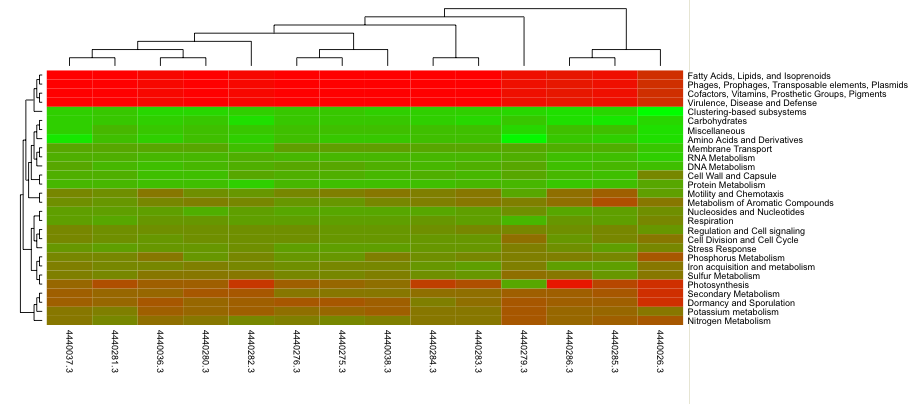
\includegraphics[width=4in]{Images/heatmap.png}
\end{center}
\caption{
Heatmap/dendogram example in MG-RAST. The MG-RAST heatmap/dendrogram has two dendrograms, one indicating the similarity/dissimilarity among metagenomic samples (x axis dendrogram) and another indicating the similarity/dissimilarity among annotation categories (e.g., functional roles; the y-axis dendrogram).
}
\label{fig:heatmap}
\end{figure}


The heatmap/dendrogram (Figure \ref{fig:heatmap}) allows an enormous amount of information to be presented in a visual form that is amenable to human interpretation. Dendrograms are trees that indicate similarities between annotation vectors. The MG-RAST heatmap/dendrogram has two dendrograms, one indicating the similarity/dissimilarity among metagenomic samples (x-axis dendrogram) and another indicating the similarity/dissimilarity among annotation categories (e.g., functional roles; the y-axis dendrogram). A distance metric is evaluated between every possible pair of sample abundance profiles. A clustering algorithm (e.g., ward-based clustering) then produces the dendrogram trees. Each square in the heatmap dendrogram represents the abundance level of a single category in a single sample. The values used to generate the heatmap/dendrogram figure can be downloaded as a table by clicking on the download button.
% %%%%%%%%%%%%%%%%%%%%%%%%%%%%%%%%%%%%%%%%%%%%%%%%%%%%%%%%%%%%%%%%%%%%%%
% %%%%%%%%%%%%%%%%%%%%%%%%%%%%%%%%%%%%%%%%%%%%%%%%%%%%%%%%%%%%%%%%%%%%%%
\subsection{Ordination}

MG-RAST uses Principle Coordinate Analysis (PCoA) to reduce the dimensionality of comparisons of multiple samples that consider functional or taxonomic annotations.
%PCoA is a well-known method for dimensionality reduction of large data sets.
Dimensionality reduction is a process that allows the complex variation found in a large datasets (e.g., the abundance values of thousands of functional roles or annotated species across dozens of metagenomic samples) to be reduced to a much smaller number of variables that can be visualized as simple two- or three-dimensional scatter plots. The plots enable interpretation of the multidimensional data in a human-friendly presentation. Samples that exhibit similar abundance profiles (taxonomic or functional) group together, whereas those that differ are found farther apart.

A key feature of PCoA-based analyses is that users can compare components not just to each other but to metadata recorded variables (e.g., sample pH, biome, DNA extraction protocol) to reveal correlations between extracted variation and metadata-defined characteristics of the samples. It is also possible to couple PCoA with higher-resolution statistical methods in order to identify individual sample features (taxa or functions) that drive correlations observed in PCoA visualizations. This coupling can be accomplished with permutation-based statistics applied directly to the data before calculation of distance measures used to produce PCoAs; alternatively, one can apply conventional statistical approaches (e.g., ANOVA or Kruskal-Wallis test) to groups observed in PCoA-based visualizations.
% %%%%%%%%%%%%%%%%%%%%%%%%%%%%%%%%%%%%%%%%%%%%%%%%%%%%%%%%%%%%%%%%%%%%%%
% %%%%%%%%%%%%%%%%%%%%%%%%%%%%%%%%%%%%%%%%%%%%%%%%%%%%%%%%%%%%%%%%%%%%%%
\subsection{Table}

The table tool creates a spreadsheet-based abundance table that can be searched and restricted by the user. Tables can be generated at user-selected levels of phylogenetic or functional resolution. Table data can be visualized by using Krona \cite{KRONA} or  can be exported in BIOM\cite{BIOM} format to be used in other tools (e.g., QIIME \cite{QIIME}).  The tables also can be exported as tab-separated text.

Abundance tables serve as the basis for all comparative analysis tools in MG-RAST, from PCoA to heatmap/dendrograms.

Consider the following example showing how to use
the taxonomic information derived from an analysis of protein similarities found for the data set 4447970.3.
We use the best hit classification, \gls{SEED} database, $10^{-5}$ evalue, 60\% identity, and a minimal alignment length of 15 amino acids. We select table output. The results are shown in Figure \ref{fig:analysis-page-table}.

The following control elements are connected to the table:
\begin{itemize}
\item group by --
allows summarizing entries below the level chosen here to be subsumed.

\item download table --
downloads the entire table as a spreadsheet.

\item Krona --
invokes KRONA \cite{KRONA} with the table data.

\item QIIME --
creates a BIOM\cite{BIOM} format file with the data being displayed in the table.

\item table size --
changes the number of elements to display for the web page.

\end{itemize}

\begin{figure}[ht]
\begin{center}
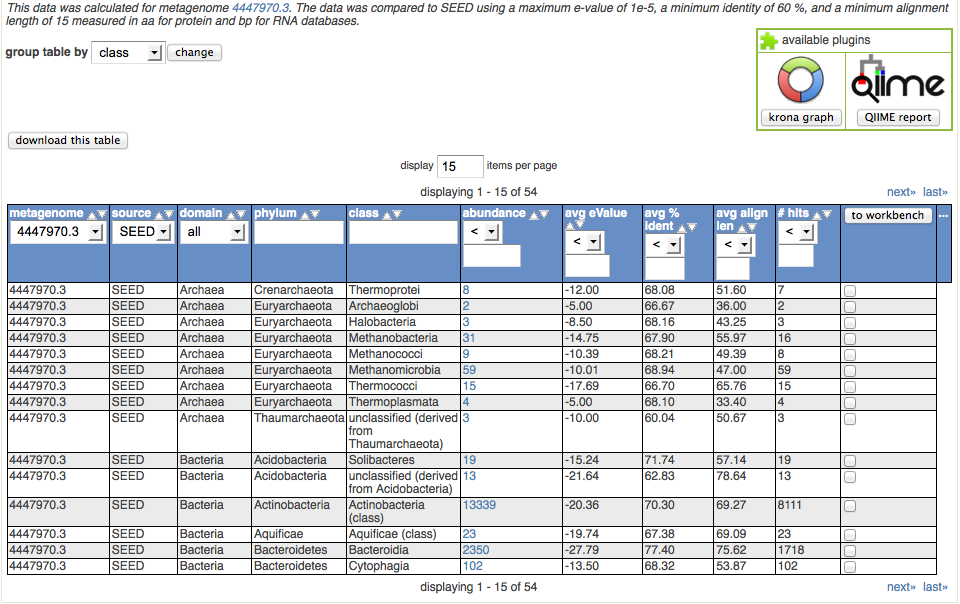
\includegraphics[width=6in]{Images/analysis-page-table.png}
\end{center}
\caption{
View of the analysis page table.
}
\label{fig:analysis-page-table}
\end{figure}

Below we explain the columns of the table and the functions available for them.
For each column we allow sorting the table by clicking on the upward- and downward-pointing triangles.

\begin{itemize}
\item metagenome

In the case of multiple datasets being displayed, this column allows sorting by metagenome ID or selection of a single metagenome.

\item source

This displays the annotation source for the data being displayed.

\item domain

The domain column allows subselecting from Archaea, Bacteria, Eukarya, and Viruses.

\item phylum, class

Since we have selected to group results at the class level, only phylum and class are being displayed. The text fields in the column headers
allow subsection (e.g., by entering Acidobacteria or Actinobacteria in the phylum field). The searches are performed inside the web browser and are efficient.

Any subselection will narrow down all datasets being displayed in the table.

Users can elect to have the results grouped by other taxonomy levels (e.g., genus), creating more columns in the table view.

\item abundance

This indicates the number of sequences found with the parameters selected matching this taxonomic unit. (Note that the parameters chosen are displayed on top of the table.) Clicking on the abundance displays another page displaying the BLAT alignments underlying the assignments.

The abundance is calculated by multiplying the actual number of database hits found for the clusters by the number of cluster members.

\item avg. evalue, avg percent identity, average alignment length

These indicate the average values for E  value, percent identity, and alignment length.

\item hits

This is the  number of clusters found for this entity (function or taxon) in the metagenome.

\item ...

This option allows extending the table to display (or hide) additional columns.

\end{itemize}
% %%%%%%%%%%%%%%%%%%%%%%%%%%%%%%%%%%%%%%%%%%%%%%%%%%%%%%%%%%%%%%%%%%%%%%
% %%%%%%%%%%%%%%%%%%%%%%%%%%%%%%%%%%%%%%%%%%%%%%%%%%%%%%%%%%%%%%%%%%%%%%
\subsection{Workbench}
The workbench was designed to allow users to select subsets of the data for comparison or export.
Specifically, the workbench supports selecting sequence features and submitting them to further analysis or other analysis. A number of use cases are described below.

An important limitation with the current implementation is that data sent to the workbench exists only until the current session is closed.
% %%%%%%%%%%%%%%%%%%%%%%%%%%%%%%%%%%%%%%%%%%%%%%%%%%%%%%%%%%%%%%%%%%%%%%
% %%%%%%%%%%%%%%%%%%%%%%%%%%%%%%%%%%%%%%%%%%%%%%%%%%%%%%%%%%%%%%%%%%%%%%
% %%%%%%%%%%%%%%%%%%%%%%%%%%%%%%%%%%%%%%%%%%%%%%%%%%%%%%%%%%%%%%%%%%%%%% 
% %%%%%%%%%%%%%%%%%%%%%%%%%%%%%%%%%%%%%%%%%%%%%%%%%%%%%%%%%%%%%%%%%%%%%%
\chapter{User Manual}
% %%%%%%%%%%%%%%%%%%%%%%%%%%%%%%%%%%%%%%%%%%%%%%%%%%%%%%%%%%%%%%%%%%%%%% 
% %%%%%%%%%%%%%%%%%%%%%%%%%%%%%%%%%%%%%%%%%%%%%%%%%%%%%%%%%%%%%%%%%%%%%% 
% %%%%%%%%%%%%%%%%%%%%%%%%%%%%%%%%%%%%%%%%%%%%%%%%%%%%%%%%%%%%%%%%%%%%%% 
\section{URL}
\url{http://metagenomics.anl.gov/}
% %%%%%%%%%%%%%%%%%%%%%%%%%%%%%%%%%%%%%%%%%%%%%%%%%%%%%%%%%%%%%%%%%%%%%% 
% %%%%%%%%%%%%%%%%%%%%%%%%%%%%%%%%%%%%%%%%%%%%%%%%%%%%%%%%%%%%%%%%%%%%%% 
% %%%%%%%%%%%%%%%%%%%%%%%%%%%%%%%%%%%%%%%%%%%%%%%%%%%%%%%%%%%%%%%%%%%%%% 
\section{Account}
The analyses of all public datasets in MG-RAST can be viewed in entirety without an MG-RAST account. An account is required to submit sequence data
for analysis or view the analyses of datasets which have been shared with you.
% %%%%%%%%%%%%%%%%%%%%%%%%%%%%%%%%%%%%%%%%%%%%%%%%%%%%%%%%%%%%%%%%%%%%%% 
% %%%%%%%%%%%%%%%%%%%%%%%%%%%%%%%%%%%%%%%%%%%%%%%%%%%%%%%%%%%%%%%%%%%%%% 
\subsection{Account registration}
Use the ``Register'' link on the front page of the website to request an account with MG-RAST, you will need to enter a unique login name and email address
along with other minimal information. Use an email address you use regularly as it will be used to communicate with you when necessary. After registering
you will receive an automated email with a temporary password after your account has been authorized, usually within a day.

If you forget your password you can request a new password on the MG-RAST website using your login and registered email address, a new password will
be generated and sent by email to this address.
% %%%%%%%%%%%%%%%%%%%%%%%%%%%%%%%%%%%%%%%%%%%%%%%%%%%%%%%%%%%%%%%%%%%%%% 
% %%%%%%%%%%%%%%%%%%%%%%%%%%%%%%%%%%%%%%%%%%%%%%%%%%%%%%%%%%%%%%%%%%%%%% 
\subsection{Account webkey}
\label{section:webkey}
The webkey is a unique string of text, e.g. ``b8Dvg2d5DCp7KsWKBPzY2GS4i'' associated with your account which is used by MG-RAST for identification
purposes. Your webkey is valid for a limited time period after which it expires and will not work anymore. You can generate a new webkey at any time, even if your current webkey has not expired.

The MG-RAST website provides two locations where you can generate a new webkey:

\begin{enumerate}
\item Log in to MG-RAST and go to the Account Management page. Press the button under �Preferences� to go the the Manage Preferences page where the Web Services section displays your current webkey with its termination date. Click on the ``generate new key'' button to generate a new key and then click the ``set preferences'' button.
\item Log in to MG-RAST and go to the Upload page and click on the ``generate webkey'' button in the ``upload files'' tab and then click on the ``generate new key'' button.
\end{enumerate}

\noindent
Note that generating a new webkey will invalidate your old webkey and your new webkey will be valid until the termination date displayed on the page.
% %%%%%%%%%%%%%%%%%%%%%%%%%%%%%%%%%%%%%%%%%%%%%%%%%%%%%%%%%%%%%%%%%%%%%% 
% %%%%%%%%%%%%%%%%%%%%%%%%%%%%%%%%%%%%%%%%%%%%%%%%%%%%%%%%%%%%%%%%%%%%%%
% %%%%%%%%%%%%%%%%%%%%%%%%%%%%%%%%%%%%%%%%%%%%%%%%%%%%%%%%%%%%%%%%%%%%%% 
\section{Uploading to MG-RAST}

MG-RAST was designed to allow users to upload sequence data directly from next-generation sequencing machines. Data can be in FASTA, FASTQ, or SFF format.

We suggest uploading raw data (in FASTQ or SFF format) and letting MG-RAST perform the quality control step because
this approach will allow us to identify any issues with the sequencing run. Frequently, local quality control will identify some
issues but mask others.

Compressing large files will reduce the upload time and the chances of a failed upload. Users can upload gzip (.gz) and bzip2 (.bz2) or Zip (.zip) files, as well as tar archives compressed with gzip (.tar.gz) or bzip2 (.tar.bz2). Note that the size of Zip files should be under 4 GB in size.

It is not necessary to assemble data prior to upload to MG-RAST. The system has been optimized for short reads and can handle uploads of many hundreds of gigabytes.

Assembled data can be uploaded to MG-RAST and read abundance information for contigs can be imported as well from FASTA files.
The ``assembled'' option for the pipeline will attempt to retrieve read abundance information from the FASTA sequence files.
% %%%%%%%%%%%%%%%%%%%%%%%%%%%%%%%%%%%%%%%%%%%%%%%%%%%%%%%%%%%%%%%%%%%%%% 
% %%%%%%%%%%%%%%%%%%%%%%%%%%%%%%%%%%%%%%%%%%%%%%%%%%%%%%%%%%%%%%%%%%%%%%
\subsection{Steps for submission via the web interface}

To start uploading data to MG-RAST through the website, click on the green up arrow. Doing so opens the Upload page.
On this page you can upload files, modify the files where needed, add metadata, and submit files for analysis.

The page is split into two sections: ``Prepare Data,'' to upload, manipulate, and assemble all the files required for a submission, and ``Submission,'' to create the MG-RAST job(s), set analysis parameters, and start the analysis. Each section contains subsections that you can click to expand.
% %%%%%%%%%%%%%%%%%%%%%%%%%%%%%%%%%%%%%%%%%%%%%%%%%%%%%%%%%%%%%%%%%%%%%%
\subsubsection{Prepare data}

All files uploaded to MG-RAST should be named using only alphanumeric and .-\_ characters without spaces. 

Files larger than 50 MB should be compressed before upload, using gzip (preferable), bzip2 or Zip (less than 4 GB in size). Compression will reduce the time taken for the upload of the file, which in turn reduces the chance that the upload will fail.

The requirements for submission are sequence information (required), metadata (strongly recommended) and barcode information (for multiplexed datasets only).

\begin{itemize}
\item {\bf Sequence files}

Sequence files must be in either FASTA, FASTQ, or SFF formats

Sequence file names must have one of the following extensions -- `.fasta', `.fna', `.fastq', `.fq', or `.sff'.

FASTA and FASTQ files should be in plain text ASCII.

FASTA files (and all sequence data submitted to MG-RAST) should not contain protein sequences.

Assembled data with read abundance information must be in FASTA format and the coverage included in the sequence ID using the following simple format:
\begin{verbatim}
>sequence_number_1_[cov=2]
CTAGCGCACATAGCATTCAGCGTAGCAGTCACTAGTACGTAGTACGTACC
>sequence_number_2_[cov=4]
ACGTAGCTCACTCCAGTAGCAGGTACGTCGAGAAGACGTCTAGTCATCAT
....
\end{verbatim}
The abundance information must be appended without spaces to the end of the sequence name (also without whitespace) in the format ``\_[cov=n]'', where n is the coverage or abundance of each contig.
Sequence files in this format should be submitted with the ``assembled'' option selected and the pipeline will retrieve read abundance information from the sequence file.

\item {\bf Metadata file}

We provide a spreadsheet template that can be filled out with all the available metadata information for a dataset, there is a link to the template on the upload page. Download the template and edit to include as much information as is available. While the number of fields in the template is large, the number of required fields, colored in red in the template, is small. The template file can be used to upload metadata for one or multiple samples and submit them to MG-RAST as a single project. The metadata can be modified at any time after submission to add information or to correct errors. See Section \ref{section:generating_metadata} for more details.

\item {\bf Barcode file}

Barcode files are required only for sequence data which will be demultiplexed on the MG-RAST website.

The barcode file should be in plain text ASCII.

Each  line of the file should contain a single barcode sequence followed by a tab and then a unique filename, with as many lines as necessary for the barcodes in the sequence file you are submitting.

\end{itemize}
% %%%%%%%%%%%%%%%%%%%%%%%%%%%%%%%%%%%%%%%%%%%%%%%%%%%%%%%%%%%%%%%%%%%%%%
\subsubsection{Upload files}

On the Upload page, in the ``upload files'' tab, click on the ``Browse'' button to select the file or files.  The upload will begin automatically after the files are selected. Once the upload has started progress bars will be displayed. If the upload does not start immediately check that you are using the latest version of FireFox.

For the actual uploading we use an HTML5 feature \cite{HTML5FILEAPI} that automatically breaks the files into chunks on the client side and sends them. Note: This is one of the reasons we request that you use a recent version of Firefox as older versions might be slower.

Based on observed values, upload times per 1 GB ($10^9$ bytes) vary from 2 minutes to over an hour, with typical times being 10 to 15 minutes. Your experience will vary depending on the speed of your connection to the internet and the quality of service in your region.

Table 1 summarizes observed upload times that might help users estimate how long the upload should take.

\begin{table}
\begin{center}
\caption{Summary of upload times}
\begin{tabular}{ l | c | r }
Technology & Rate (bit/s) & Time for 1GB Upload\\
  \hline
Modem 14.4 (2400 baud) &	14.4 kbit/s&	154 hours\\
ADSL Lite & 1.5 Mbit/s &	1.5 hours\\
Ethernet&	10 Mbit/s & 13.33 minutes\\
T3 &	44.736 Mbit/s &~3 minutes\\
Fast Ethernet &	100 Mbit/s &1.33 minutes\\
  \hline
\end{tabular}
\end{center}
\end{table}

\noindent
{\bf Verifying the integrity of the uploaded files.}

When the upload of your files has completed, you will be prompted with the \gls{MD5}-sum of each file. You should generate an MD5 sum for each uploaded file on your machine, paste it into the appropriate box in the prompt, and click the ``check" button (see Figure 4.1). A popup will show you whether there is a match; additionally the check button will turn green upon success and red upon failure. Click the ``Close" button if you have completed the checks or if you wish to skip this step.

\begin{figure*}[ht]
\begin{center}
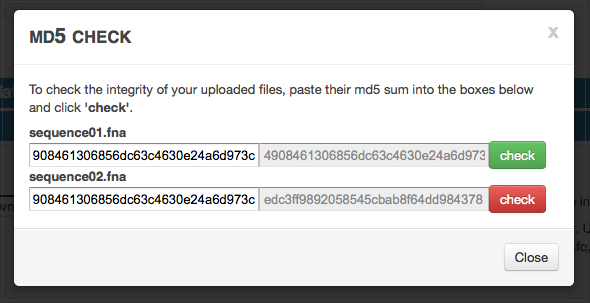
\includegraphics[width=4in]{Images/upload-page-md5-verification.png}
\end{center}
\caption{
Dialogue requesting the user to put in a locally generated \gls{MD5} checksum for the files to identify any data corruption during the upload.
}
\label{fig:upload-page-md5-verification}
\end{figure*}

Checking the integrity especially of large files is important because it will give you immediate feedback about whether your upload was successful. If not detected at upload time, a damaged file will lead to errors later in the pipeline, wasting both valuable compute cycles and, even more important, your time. To generate an \gls{MD5} sum of your file, you can use the ``md5" shell command on a Mac, the ``md5sum" shell command on Unix systems, or the freely available md5-sum tools on Windows (e.g., from http://www.winmd5.com/).

\noindent
{\bf File filters in place for uploaded files.}

Since MG-RAST has been designed to work with metagenomic and metatranscriptomic datasets, there is a filter in place trying to identify
datasets not suitable for MG-RAST. Those datasets will be colored red in the inbox listing and cannot be submitted.
Following are the criteria for rejection:

\begin{itemize}
\item Protein sequences --
MG-RAST is optimized to perform translation from DNA to proteins.

\item Reads shorter than 75 basepairs --
The gene prediction stage performance deteriorates significantly with shorter reads.

\item genomes --
Submissions with complete genomes or a small number of contigs are rejected as well. Here our sister service RAST at \url{http://rast.nmpdr.org} should be used instead of MG-RAST.

\item Files that are too small (sequence data less than 1 Mbp) --
Files that are too small for MG-RAST to properly function are rejected at the submission stage. The minimal size requirement is 1 megabasepair.

\item Corrupted files --
FASTA and FASTQ files which do not conform to the format standard, e.g. if the number of unique identifiers does not match the number of sequence records in a file, the file is considered corrupt.

\item Alignments --
We cannot identify proteins from sequences containing alignment information.

\item Colorspace --
The tool chain does not function for ABIsolid sequences in colorspace. Please translate to standard FASTA.

\item rar compressed files and Zip files over 4 GB --
We cannot decompress these files.

\end{itemize}

In addition we will filter at the upload stage any Word documents, Rich Text Format files, and all
files without the extension .fna, .fasta, .fq, .fastq, or .sff in their name.


\textbf{Note:} We recommend computing an \gls{MD5} checksum and verifying that the checksum computed by MG-RAST is identical to the locally computed checksum. This is the best way to ensure data integrity.

All files uploaded to MG-RAST will be displayed in your inbox and you can perform certain operations on them. Compressed and/or archived files must be unpacked, SFF files must be converted to FASTQ, and sequence data can be demultiplexed using barcodes contained in an uploaded barcode file. Files can also be deleted. See Section \ref{section:managing_the_inbox} for more details.

When a sequence file is selected, some information about the sequence data is displayed, see Figure \ref{fig:Inbox-File-Information}. It is a good idea to check that the uploaded files in your inbox match your local copies. The file \gls{MD5} checksum, file size, sequence count, and basepair count can be used for this purpose.


\textbf{Please note:} After the actual upload is complete, the system will compute the statistics shown in Figure \ref{fig:Inbox-File-Information}. Computing this information takes some time, so the statistics for your sequence files will not be visible immediately after you uploaded it. If the statistics are not displayed in a reasonable time refresh your browser page to trigger the statistics computation.
% %%%%%%%%%%%%%%%%%%%%%%%%%%%%%%%%%%%%%%%%%%%%%%%%%%%%%%%%%%%%%%%%%%%%%%
\subsubsection{Submission}
The submission process allows you to create MG-RAST jobs using files in your inbox. It is designed to facilitate the creation of a large number of jobs easily.

\begin{itemize}

\item {\bf Select metadata file}

We recommend you supply metadata for all your samples. We assign a higher processing priority to samples with metadata. Metadata files that have successfully passed our validation step will be displayed for selection.

\item {\bf Select project}

All jobs created in MG-RAST will need to be placed in a project---either an existing project or a new one created by you during the submission. The project can be specified in one of three ways: in the metadata file if supplied or selected from the existing projects you have access to, or a new project name can be entered into the text box.

\item {\bf Select sequence file(s)}

All FASTA and FASTQ sequence files in your inbox will be displayed for selection and job submission. Each sequence file can be used to create a single MG-RAST job. SFF files must be converted to FASTQ and the FASTQ file will be used for the submission.

\item {\bf Choose pipeline options}

The MG-RAST analysis can be influenced by the options selected here, which affect dereplication, screening, and quality of the filtering of the reads. The options selected are applied to all the sequence files selected.

\item {\bf Submit job}

This is the final step after which the analysis pipeline takes over and the processing begins. Once the job or jobs have been submitted, all the files required to create them will be removed from your inbox.

\end{itemize}

\noindent
You can monitor the progress of your jobs in ``My Data Summary" on the Browse Metagenomes page.
% %%%%%%%%%%%%%%%%%%%%%%%%%%%%%%%%%%%%%%%%%%%%%%%%%%%%%%%%%%%%%%%%%%%%%% 
% %%%%%%%%%%%%%%%%%%%%%%%%%%%%%%%%%%%%%%%%%%%%%%%%%%%%%%%%%%%%%%%%%%%%%%
\subsection{Cmd-line uploader}

The following syntax will allow uploading to MG-RAST from the command line.

\begin{verbatim}
curl -H "auth: webkey" -X POST -F "upload=@/path_to_file/
metagenome.fasta" "http://api.metagenomics.anl.gov/
inbox/upload" > curl_output.txt
\end{verbatim}
where you need to substitute ``webkey'' (see Section \ref{section:webkey}) with the unique string of text generated by MG-RAST for your account. Your webkey is valid for a limited time period and ensures that the uploads you perform from the command line are recognized as belonging to your MG-RAST account and are placed in the correct inbox.
% %%%%%%%%%%%%%%%%%%%%%%%%%%%%%%%%%%%%%%%%%%%%%%%%%%%%%%%%%%%%%%%%%%%%%%
% %%%%%%%%%%%%%%%%%%%%%%%%%%%%%%%%%%%%%%%%%%%%%%%%%%%%%%%%%%%%%%%%%%%%%%
\subsection{Managing the Inbox}
\label{section:managing_the_inbox}

The Inbox is a temporary storage location for sequence and metadata files prior to submission to the pipeline, see Figure \ref{fig:Inbox}. To protect us from any
misuse of the facility, we have limited the Inbox to metadata spreadsheets and sequence files.

\noindent
Files are visible only to the uploading user and will automatically be deleted after 72 hours.

\begin{figure*}
\begin{center}
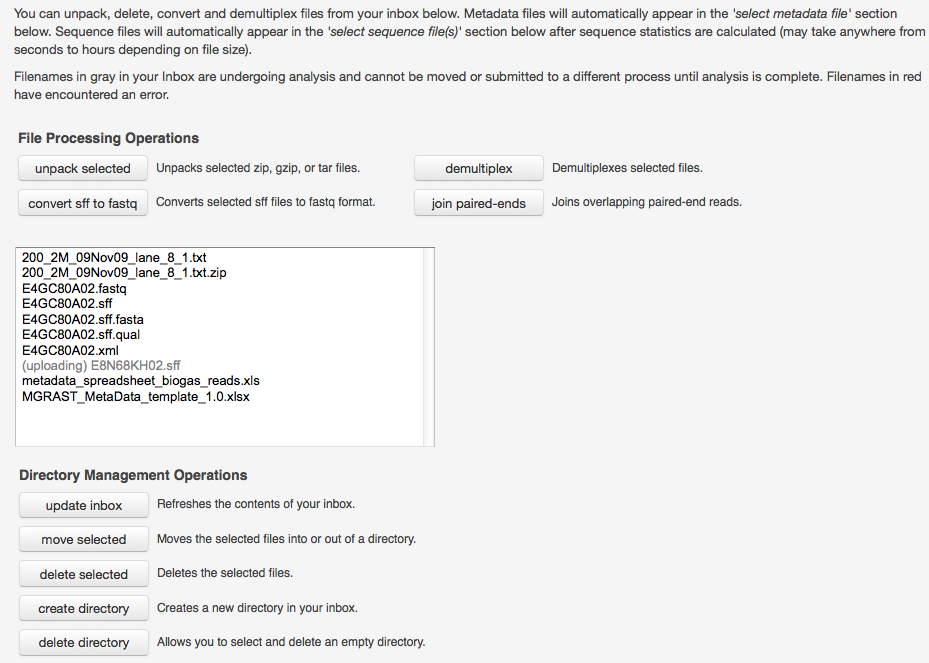
\includegraphics[width=6in]{Images/Inbox.png}
\end{center}
\caption{
Temporary storage provided in Inbox before submitting data and limited editing features.
}
\label{fig:Inbox}
\end{figure*}
% %%%%%%%%%%%%%%%%%%%%%%%%%%%%%%%%%%%%%%%%%%%%%%%%%%%%%%%%%%%%%%%%%%%%%% 
\subsubsection{File-processing options in the Inbox}
The following file-processing options are available. 
\begin{itemize}
\item unpack selected --
unpacks selected zip, gzip, bzip2 files and tar archives compressed with gzip or bzip2.
\item convert SFF to FASTQ --
converts selected SFF files to FASTQ format (only FASTQ and FASTA files can be submitted to the system).
\item demultiplex --
demultiplexes selected files.

Note that this is suitable only for 454 type barcodes that are actual prefixes of the reads. This approach does not work for the Illumina barcode approach (basically a third read for each paired end read).

\item join paired ends --
joins overlapping paired-end reads.
\end{itemize}

\noindent
{\bf Demultiplexing for 454 and similar datasets}:

MG-RAST performs demultiplexing based on the presence of the barcode sequence at the beginning of the reads.
Assume you have a sequence file testseq.fasta and your barcode file has tab-separated lines like the following.
\begin{verbatim}
AAAAAAAA     fileA
CCCCCCCC     fileC
\end{verbatim}
The demultiplexing step will split your sequence file into three files:
fileA.fasta containing all the reads that begin with AAAAAAAA,
fileC.fasta containing all the reads that begin with CCCCCCCC,
and
testseq\_no\_MID\_tag.fasta containing reads that do not match either of the two.

We note that demultiplexing for Illumina needs to be done outside the MG-RAST system. Illumina barcodes work differently from 454 barcodes.
% %%%%%%%%%%%%%%%%%%%%%%%%%%%%%%%%%%%%%%%%%%%%%%%%%%%%%%%%%%%%%%%%%%%%%% 
\subsubsection{Directory management operations for the Inbox}
The following operations are available for managing the directory.

\begin{itemize}
\item update inbox --
refreshes the contents of your inbox
\item move selected --
 moves the selected files into or out of a directory
\item delete selected --
deletes the selected files
\item create directory --
creates a new directory in your inbox
\item delete directory --
allows you to select and delete an empty directory.
\end{itemize}

Users should always double check the \gls{MD5} checksum for files that are uploaded to the system in order to verify the integrity. Figure \ref{fig:Inbox-File-Information} shows the MD5 fingerprint that is computed upon upload for each file.

\begin{figure*}
\begin{center}
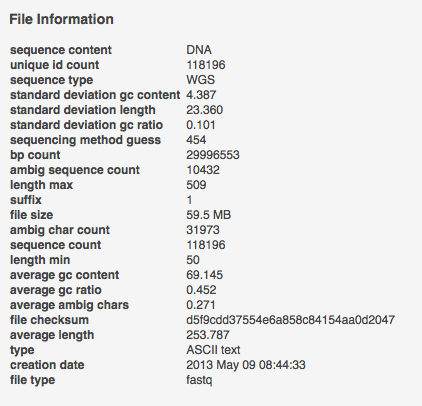
\includegraphics[width=4in]{Images/Inbox-File-Information.png}
\end{center}
\caption{
Information displayed by the inbox for one file (once selected).
}
\label{fig:Inbox-File-Information}
\end{figure*}
% %%%%%%%%%%%%%%%%%%%%%%%%%%%%%%%%%%%%%%%%%%%%%%%%%%%%%%%%%%%%%%%%%%%%%% 
% %%%%%%%%%%%%%%%%%%%%%%%%%%%%%%%%%%%%%%%%%%%%%%%%%%%%%%%%%%%%%%%%%%%%%%
\subsection{Generating metadata for the submission}
\label{section:generating_metadata}

MG-RAST uses questionnaires to capture metadata for each project with one or more samples. Users download and fill out the questionnaire and then submit it.
Questionnaires are validated
automatically by MG-RAST
for completeness and compliance with the controlled vocabularies for certain fields.

MG-RAST has implemented the use of Minimum Information about any (X) Sequence (MIxS)\cite{MIENS} developed by the Genomic Standards Consortium. In addition to the minimal checklists, more detailed data can be captured in optional environmental packages.

We use simple spreadsheets to capture metadata, with a minimal number of required fields (in red in the spreadsheets) and a number of optional fields. The spreadsheet is separated into multiple tabs representing the different metadata categories. The MG-RAST metadata spreadsheet template is available on the MG-RAST upload page or at \url{ftp://ftp.metagenomics.anl.gov/data/misc/metadata/MGRAST_MetaData_template_1.3.xlsx}.

A filled-out version of the spreadsheet is available at \url{ftp://ftp.metagenomics.anl.gov/data/misc/metadata/MGRAST_MetaData_template_example.xlsx}.

In Figure \ref{fig:project-spreadsheet} we show the template tab for project and the required field labels (in red) (in essence, your contact information).
Figure \ref{fig:project-spreadsheet-multiple-tabs} shows the various tabs in the spreadsheet.

\begin{figure*}[ht]
\begin{center}
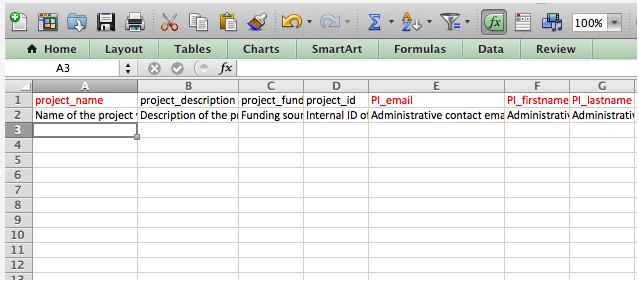
\includegraphics[width=6in]{Images/project-spreadsheet.png}
\end{center}
\caption{
Project spreadsheet. In red are required fields. Note that the 2nd row contains information on how to fill out the form.
}
\label{fig:project-spreadsheet}
\end{figure*}

\begin{figure*}[ht]
\begin{center}
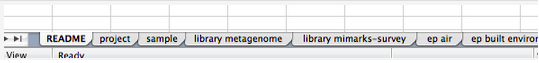
\includegraphics[width=6in]{Images/project-spreadsheet-multiple-tabs.png}
\end{center}
\caption{
The various tabs in the spreadsheet. Project, sample and one of library metagenome or library mimarks survey are required.
}
\label{fig:project-spreadsheet-multiple-tabs}
\end{figure*}

Note: Use the third line in the spreadsheet and as shown in Figure \ref{fig:project-spreadsheet-with-3-samples} to enter your data. Do not attempt to alter the first two lines or delete them; they are read only. The first line contains the field labels, and the second line contains descriptions that can help explain how to fill out the fields, along with what unit to use (e.g., temperature in Celsius and distance in meters), URL for the bioportal ontology site etc..

\begin{figure*}[ht]
\begin{center}
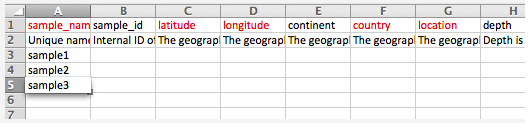
\includegraphics[width=6in]{Images/project-spreadsheet-with-3-samples.png}
\end{center}
\caption{
Sample tab with 3 new samples (sample1, sample2, and sample3) added. Again red text in the first row indicates required fields. Rows 1 and 2 cannot be altered.
}
\label{fig:project-spreadsheet-with-3-samples}
\end{figure*}

\subparagraph*{Required sheets}
You need to fill out four sheets to describe your metadata:

\begin{enumerate}
\item Project --
This sheet has only one row, and describes a set of samples uploaded together; the other sheets have one row per sample.

\item Sample --
This sheet includes either the filename or metagenome name used for matching.

\item Library --
This sheet includes either the metagenome (for WGS and WXS), mimarks-survey (for \gls{16s} and amplicon) or metatranscriptome.

\item Environmental package (ep) --
Several packages of suggested standard metadata are available.
Choose the package that best describes your dataset (e.g., water, human-skin, soil).

\end{enumerate}

\subparagraph*{Sample sheet}
The sample sheet requires minimal information (including the sample name) about where and when the sample was taken. Note that some fields in the spreadsheet must be filled out with terms from a controlled vocabulary or in a certain way. Country and environment (biome, feature, material) fields require entries from curated ontologies, gazetteer and environmental ontology, respectively.

Figure \ref{fig:project-spreadsheet-with-3-samples}
shows the sample tab with three new samples (sample1, sample2, and sample3) added. Again red text in the first row indicates required fields.

\subparagraph*{Mandatory fields}
Five fields must be completed.
\begin{itemize}
\item Country --
e.g. United States of America, Netherlands, Australia, Uruguay
\item Latitude and longitude -- 
e.g. [106.84517, -104.60667], [28° 42.306′N, 88° 24.099′W], [45.30 N, 73.35 W]
\item Biome --
e.g. small lake biome, urban biome, mangrove biome. This term must be one of the terms from the bioportal ontology (\url{http://bioportal.bioontology.org/ontologies/1069?p=terms&conceptid=ENVO\%3A00000428}). Terms that are not listed on this site are not valid.
\item Feature --
e.g. city, fish farm, livestock-associated habitat, marine habitat, ocean basin, microbial mat. This term must be one of the terms from the bioportal ontology. Terms that are not listed on this site are not valid.
\item Material --
e.g. air, dust, volcanic soil, saliva, blood, dairy product, surface water, piece of gravel. This term must be one of the terms from the bioportal ontology. Terms that are not listed on this site are not valid.
\end{itemize}

\subparagraph*{Library section}
The library section captures technical data on the preparation and sequencing done. You should choose the library tab to fill out (``metagenome'' for shotgun sequencing, ``mimarks-survey'' for amplicon or ``metatranscriptome") based on the type of sequencing done. These are separated as different sequencing techniques involving different metadata fields. Each row describes one library for one sample. The required fields are colored red.

The \textbf{sample\_name} value in the library sheet must exactly match one of the values used in the sample sheet.

The \textbf{file\_name} field holds the filename of the sequence file uploaded, or the filename to use for creating the demultiplexed file if you uploaded a multiplexed sequence file and have barcode sequences in the spreadsheet. This is used for mapping sequence files to metadata.

The \textbf{metagenome\_name} field holds the name of the metagenome you are submitting. If the file\_name field is empty, the metagenome\_name will be used to map metadata to sequence files, in this case it would need to match the uploaded sequence filename without the file extension, e.g. a sequence file ``test-sequence.fasta" would be mapped to the metadata in the row which has the metagenome\_name value ``test-sequence".

The \textbf{investigation\_type} field is required to be ``metagenome'' for shotgun metagenome samples, ``mimarks-survey'' for amplicon studies or ``metatrascriptome", reflecting which tab was filled out.

The type of sequencing instrument used is another required field. Values are, for example, Sanger, pyrosequencing, ABI-solid, 454, Illumina, assembled, other.

Again, only a limited number of fields are required. However, the more information you provide, the easier it is for you and others to understand any potential uses of your data and to understand why results appear in a particular way. It might, for example, allow understanding of specific biases caused by technology choices or sampled environments.

\subparagraph*{Environmental Package (ep) sheet}
You can fill out one or more environmental metadata packages.  Currently we provide support for the following GSC environmental packages:

\begin{itemize}\addtolength{\itemsep}{-.55\baselineskip}
\item Air
\item Built Environment
\item Host-associated
\item Human-associated
\item Human-oral
\item Human-skin
\item Human-gut
\item Human-vaginal
\item Microbial mat/biofilm
\item Miscellaneous natural or artificial environment
\item Plant-associated
\item Sediment
\item Soil
\item Wastewater sludge
\item Water
\end{itemize}

We strongly encourage users to submit rich metadata, but we understand the effort required in providing it. Using the environmental packages (which were designed and are used by practitioners in the respective field) should make it reasonably simple to report the essential metadata required to analyze the data. If there is no environmental package to report metadata for your specific sample, please contact MG-RAST staff: we will work with the GSC\cite{GSC} to create the required questionnaire.
% %%%%%%%%%%%%%%%%%%%%%%%%%%%%%%%%%%%%%%%%%%%%%%%%%%%%%%%%%%%%%%%%%%%%%% 
% %%%%%%%%%%%%%%%%%%%%%%%%%%%%%%%%%%%%%%%%%%%%%%%%%%%%%%%%%%%%%%%%%%%%%% 
% %%%%%%%%%%%%%%%%%%%%%%%%%%%%%%%%%%%%%%%%%%%%%%%%%%%%%%%%%%%%%%%%%%%%%%
 \section{Working with Projects and Collections}

Collections provide an efficient way to create multiple sets of metagenomes for analysis. For example, if you want to compare human gut with cow rumen samples, you probably want to see a dialogue like that in Figure \ref{fig:collections-total-list1}.

\begin{figure*}[ht]
\begin{center}
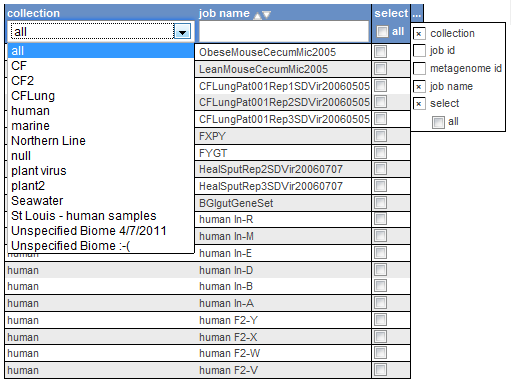
\includegraphics[width=6in]{Images/collections-total-list1.png}
\end{center}
\caption{
View of the browse table with the collection column enabled. Clicking on the ``..." at the right end of the table allows expanding the table columns.
}
\label{fig:collections-total-list1}
\end{figure*}

MG-RAST v3 provides a mechanism to make this happen. Users can create collections that are persistent across multiple sessions.
Below, we show how to define a collection that allows comparison of multiple datasets. Please note that collections are just shortcuts to the actual samples; they cannot be shared at this time.

Step 1: you start with the metadata browser (either on the front page or in the little menu block in the top right-hand corner), and click on the globe symbol. See Figure \ref{fig:browse-for-metagenomes} for the symbol.

\begin{figure*}[ht]
\begin{center}
\includegraphics[width=2in]{Images/browse-for-metagenomes.png}
\end{center}
\caption{
Symbol for the MG-RAST metagenome browser}
\label{fig:browse-for-metagenomes}
\end{figure*}

Step 2: This will take you to the Browser dialogue, showing a large number of metagenomes (Figure \ref{fig:browse-window}).

\begin{figure*}
\begin{center}
\includegraphics[width=4in]{Images/collections-browse-window.png}
\end{center}
\caption{
MG-RAST metagenome browser}
\label{fig:browse-window}
\end{figure*}

Step 3: Clicking on biome will allow selecting a specific Biome (here we pick Animal associated).
This results in a list of metagenomes shown in 
Figure \ref{fig:collections-filter-by-biome}.

\begin{figure*}
\begin{center}
\includegraphics[width=6in]{Images/collections-filter-by-biome.png}
\end{center}
\caption{
Filtering by BIOME information. }
\label{fig:collections-filter-by-biome}
\end{figure*}

The list of samples still shows too many samples when restricted to just animal associated metagenomes.

\begin{figure*}
\begin{center}
\includegraphics[width=4in]{Images/collections-filtered-but-too-many.png}
\end{center}
\caption{
A reduced list of metagenomes for one BIOME. }
\label{fig:collections-filtered-but-too-many}
\end{figure*}

Step 4: To downselect, search for Twin to further restrict to samples from Peter Turnbaugh and Jeffrey Gordon's Human Twin study (see Figure \ref{fig:collections-twin}).

\begin{figure*}[ht]
\begin{center}
\includegraphics[width=6in]{Images/collections-twin.png}
\end{center}
\caption{
Selecting a specific project to further reduce the number of datasets being displayed. }
\label{fig:collections-twin}
\end{figure*}

Step 5: Clicking on the black shopping-cart symbol in the top right-hand corner will allow the creation of a new collection entry. The next step is naming the collection (see Figure \ref{fig:Collections-how-to-save}.
Here we name the collection Twin Study and hit OK.

\begin{figure*}[ht]
\begin{center}
\includegraphics[width=6in]{Images/Collections-how-to-save.png}
\end{center}
\caption{
Saving a collection}
\label{fig:Collections-how-to-save}
\end{figure*}

Step 6: Once the collection is added, the new collection will appear in the list of collections (in ``Your Data Summary").

\begin{figure*}[ht]
\begin{center}
\includegraphics[width=6in]{Images/collections-finished.png}
\end{center}
\caption{
List of collections}
\label{fig:collections-finished}
\end{figure*}

Step 7: Use collection in the Metagenome selection on the Analysis page. It is possible to analyze individual metagenomes or compare whole groups of metagenomes (see Figure \ref{fig:using-collections}).

\begin{figure*}[ht]
\begin{center}
\includegraphics[width=6in]{Images/using-collections.png}
\end{center}
\caption{
Comparing collections as groups.}
\label{fig:using-collections}
\end{figure*}
% %%%%%%%%%%%%%%%%%%%%%%%%%%%%%%%%%%%%%%%%%%%%%%%%%%%%%%%%%%%%%%%%%%%%%%
% %%%%%%%%%%%%%%%%%%%%%%%%%%%%%%%%%%%%%%%%%%%%%%%%%%%%%%%%%%%%%%%%%%%%%% 
% %%%%%%%%%%%%%%%%%%%%%%%%%%%%%%%%%%%%%%%%%%%%%%%%%%%%%%%%%%%%%%%%%%%%%%
\section{Understanding Datasets}
Unfortunately not every sequencing run works equally well. Users of MG-RAST have provided data with
many different sources of error, allowing us to provide a number of tools to identify the most common errors.

The quality assessment tools described in Section \ref{section:Quality} provide a good tool set for an initial data quality analysis. While many potential sources of error exist, some common problems can be easily identified with just the nucleotide histograms. If your data exhibits patterns like the ones described in Section \ref{section:Quality}, there were likely to be problems with sequencing.
% %%%%%%%%%%%%%%%%%%%%%%%%%%%%%%%%%%%%%%%%%%%%%%%%%%%%%%%%%%%%%%%%%%%%%%
%\subsection{Why are so many reads failing QC?}

We frequently find datasets with high numbers of reads filtered out by the quality control. Below we list the major reasons for filtered reads:

\begin{enumerate}
\item Artificial duplicate reads 

The presence of significant amounts of ADRs hints at problems with a PCR step. Frequently a problem with 454 runs occurs, but problems are also seen with other platforms. For example, a set of DNA templates may be  copied many times during a PCR step, often consuming up to 80\% of the entire dataset.

\item Filtered reads

If you have selected screening against a host organism (e.g., the human genome), reads matching that particular genome will be removed from the dataset. This action frequently consumes a large fraction of the sequence run. There are in vitro techniques to minimize the amount of host DNA in your sample. see \cite{THOMASREVIEW}.

\item Filter rRNA reads in metatranscriptomes

If you are trying to analyze a metatranscriptome, reducing the amount of ribosomal is essential. Unless an in vitro rRNA knockdown method is applied, up to 97\% of all reads will be ribosomal.
\end{enumerate}
% %%%%%%%%%%%%%%%%%%%%%%%%%%%%%%%%%%%%%%%%%%%%%%%%%%%%%%%%%%%%%%%%%%%%%% 
% %%%%%%%%%%%%%%%%%%%%%%%%%%%%%%%%%%%%%%%%%%%%%%%%%%%%%%%%%%%%%%%%%%%%%%
% %%%%%%%%%%%%%%%%%%%%%%%%%%%%%%%%%%%%%%%%%%%%%%%%%%%%%%%%%%%%%%%%%%%%%%
\section{Drilling Down with the Workbench}

One of the new features of MGRAST v3 is the workbench. It is the main mechanism for exchanging subsets of data between analysis views. It also allows you to download the FASTA files of a selection of proteins.

When you initially go to the Analysis page (see Section \ref{section:analysis-page}), your workbench will be empty. It is displayed as the leftmost tab in the data tabular view. So how do you get data into the workbench? There are two simple ways to select data subsets: from any generated table or from the drilldown of a barchart.

Try this example: Start by selecting the lean and obese mouse cecum samples (MG-RAST IDs 4440463.3 and 4440464.3) \cite{OBESEMICE} in the data selection and creating a table. To do so, go to the Analysis page, and select the analysis view Organism Classification. Expand the metagenome selection by clicking the plus symbol next to metagenomes. Select public from the dropdown-box (to view only public data sets), and type ``mouse'' into the filter box. Select the two samples, and click the button with the right arrow, then the ok button. The default data visualization is ``table,'' so you can click the ``generate'' button (Figure \ref{fig:analysis-page-selecting-lean-and-obese}).

\begin{figure*}
\begin{center}
\includegraphics[width=6in]{Images/analysis-page-selecting-lean-and-obese.png}
\end{center}
\caption{
Screenshot of the Analysis page and Workbench tab. Users can search and select metagenomes to analyze, the annotation sources and parameters to set, and the analysis and visualization they want to perform.
}
\label{fig:analysis-page-selecting-lean-and-obese}
\end{figure*}

After a short wait, a new tab will appear in the tabview, showing the data table with organism classifications for the two samples. The last column of this table will have a button labeled ``to workbench'' as the column header. Each cell in that column will have a checkbox. Checking a checkbox and clicking the ``to workbench'' button will send the proteins identified by that row to the workbench.
Note that you have only one workbench and that putting a new set of proteins into it will replace the current content. What if you want to select all Bacteria: do you really need to click through all those checkboxes? No: you can use the grouping feature of the table, so you have to click only one checkbox per metagenome.

Above the table you will find a dropdown-box labeled ``group table by'' (Figure \ref{fig:table-group-by-class}). Select ``domain,'' and the table will be grouped, so there is only one row per metagenome and domain.
\begin{figure}[ht]
\begin{center}
\includegraphics[width=2in]{Images/table-group-by-class.png}
\end{center}
\caption{
Using the tables to group results.
}
\label{fig:table-group-by-class}
\end{figure}

Now check the two boxes in the ``Bacteria'' rows, and click the ``to workbench'' button (see Figure \ref{fig:table-organism-abundance}.

\begin{figure}
\begin{center}
\includegraphics[width=3in]{Images/table-organism-abundance.png}
\end{center}
\caption{
Use the table to select results you want to add to your workbench for further analyses.
}
\label{fig:table-organism-abundance}
\end{figure}

A pop-up message will appear, telling you how many proteins have been sent to the workbench. If you look at the tabular view now, you will notice that the workbench tab shows the number of proteins it currently contains (see Figure \ref{fig:workbench}). If you click on that tab, you will get information about what the workbench contains. On this tab you will also find a ``download as FASTA'' button.

\begin{figure}
\begin{center}
\includegraphics[width=3in]{Images/workbench.png}
\end{center}
\caption{
View of the workbench with a summary of the proteins that have been added.
}
\label{fig:workbench}
\end{figure}

Besides being able to download the sequences of your selected proteins, you can also use them to generate other visualizations. For example, you can switch from organism to functional classification. To do so, simply check the ``use proteins from workbench'' box in the data selection when generating a new visualization (e.g., a circular tree using the proteins we just buffered).

The table is not the only visualization that allows you to put a subselection into the workbench. You can also use the barchart for this purpose (Figure \ref{fig:barchart-from-workbench}). Simply click on the ``to workbench'' button next to the headline of a drilldown. Note that you cannot put the topmost barchart into the workbench because it is not yet a subselection of proteins.

\begin{figure}
\begin{center}
\includegraphics[width=3in]{Images/barchart-from-workbench.png}
\end{center}
\caption{Using barcharts to download or add results to workbench.}
\label{fig:barchart-from-workbench}
\end{figure}

\section{Downloads from the Workbench}

The workbench feature stores subselections of data and allows those to be used as input for further selection or displays: for example, select all E. coli reads and then display the functional categories present just in E. coli reads across multiple data sets. In addition, the workbench allows downloading the annotated reads for the subselection stored in the workbench as fasta (Figure \ref{fig:workbench-download}).

\begin{figure}
\begin{center}
\includegraphics[width=3in]{Images/workbench-download.png}
\end{center}
\caption{
Download of selected reads, via the workbench, using the name space of the selection.
}
\label{fig:workbench-download}
\end{figure}

Once processing datasets in MG-RAST is finished, a download page is created for the project. On this page all data products created during the computation are made available as files. In addition, datasets that have been published in MG-RAST have links to an ftp site at the top of this page where you can download additional information.
%\subsection{How to compare metagenomes for a specific Subsystem}

%\textbf{provide an answer to the question: I understood how to make a collections of metagenomes to query but could not figure out if it was possible to limit the comparison to the roles in a SS.}
% %%%%%%%%%%%%%%%%%%%%%%%%%%%%%%%%%%%%%%%%%%%%%%%%%%%%%%%%%%%%%%%%%%%%%% 
% %%%%%%%%%%%%%%%%%%%%%%%%%%%%%%%%%%%%%%%%%%%%%%%%%%%%%%%%%%%%%%%%%%%%%% 
% %%%%%%%%%%%%%%%%%%%%%%%%%%%%%%%%%%%%%%%%%%%%%%%%%%%%%%%%%%%%%%%%%%%%%%
\section{Viewing Evidence}

For individual proteins, the MG-RAST page allows users to retrieve the sequence alignments underlying the annotation transfers (see Figure \ref{fig:blat-alignment}).
Using the M5nr \cite{M5NR} technology, users can retrieve alignments against the database of interest with no additional overhead.

\begin{figure*}[ht]
\begin{center}
\includegraphics[width=6in]{Images/blat-alignment.png}
\end{center}
\caption{
BLAT hit details with alignment.
}
\label{fig:blat-alignment}
\end{figure*}
% %%%%%%%%%%%%%%%%%%%%%%%%%%%%%%%%%%%%%%%%%%%%%%%%%%%%%%%%%%%%%%%%%%%%%% 
% %%%%%%%%%%%%%%%%%%%%%%%%%%%%%%%%%%%%%%%%%%%%%%%%%%%%%%%%%%%%%%%%%%%%%% 
% %%%%%%%%%%%%%%%%%%%%%%%%%%%%%%%%%%%%%%%%%%%%%%%%%%%%%%%%%%%%%%%%%%%%%%
\section{MG-RAST Output}

Users can access the data in MG-RAST in three ways.
\begin{itemize}
\item Through the website (which is authenticated)
\item Through the MG-RAST API (which is also authenticated)
\item Through the ftp site (which is not authenticated, and for which we put
only data from public projects)
\end{itemize}

\begin{table}
\caption{Differences between the various access modalities}
\label{table:access-modalities}
\begin{tabular}{l|c|c|c|l}
Service & Web Interface & API & FTP Server & Comment\\
 \hline
public data  access  	  &  Y                   &  Y     &  Y &\\
private data  access   &  Y                   &  Y     &  N &\\
upload                      &  Y                    &  T     & N & Unless specifically arranged by help desk\\
 \hline
\end{tabular}
\end{table}

Access to private or shared data requires either password access via the web interface or a webkey generated for access via the API.
All of the data files available on the website would be available via the urls returned by
a query to
http://api.metagenomics.anl.gov/1/download/mgm4450212.3
This returns a JSON data structure with urls for all the data files. For instance, the file
900.abundance.organism.gz
can be retrieved from
http://api.metagenomics.anl.gov/1/download/mgm4450212.3?file=900.5
Note: This is a public job which requires no authorization; private jobs can be accessed by providing your valid account webkey in the auth field in the GET request.

In general, we preserve the inputs and outputs for every stage of the pipeline for download and to ensure reproducibility.
An example of why this is useful is the use of dereplicated reads for error estimation by DRISEE (see Section \ref{section:DRISEE}) or the LCA (see Section \ref{section:LCA}) algorithm being used to reinterpret the similarities for a given cluster.
% %%%%%%%%%%%%%%%%%%%%%%%%%%%%%%%%%%%%%%%%%%%%%%%%%%%%%%%%%%%%%%%%%%%%%% 
% %%%%%%%%%%%%%%%%%%%%%%%%%%%%%%%%%%%%%%%%%%%%%%%%%%%%%%%%%%%%%%%%%%%%%%
\subsection{Data products on the website}

Users can obtain 
various data products from the website.
\begin{itemize}
\item
Spreadsheets.
Many of the web pages provide spreadsheets for download with the information rendered into tables or
graphical displays.
While most of the graphics can be downloaded directly, some require creating a static version for download (which can be achieved through a button next to the graphic).
Note that the option to use a screenshot will provide images at screen resolution.
\item
BIOM file format exports.
From the table on the Analysis page, users can download streams in BIOM~\cite{BIOM} format, reflecting the parameter choices made.
Using this approach, users can download abundance profiles in BIOM format, which can then be processed downstream with BIOM-compliant tools (e.g., QIIME \cite{QIIME}).
\item
Sequence files via the workbench.
The workbench allows download of small subsets of sequences with annotations.
\end{itemize}
% %%%%%%%%%%%%%%%%%%%%%%%%%%%%%%%%%%%%%%%%%%%%%%%%%%%%%%%%%%%%%%%%%%%%%% 
% %%%%%%%%%%%%%%%%%%%%%%%%%%%%%%%%%%%%%%%%%%%%%%%%%%%%%%%%%%%%%%%%%%%%%%
\subsection{FTP server}

All public data is made available on the FTP server.
The FTP server provides a number of services:

\begin{itemize}
\item project --
area where public data is made available for download, sorted into projects

\item data --
data created to enable MG-RAST (e.g., the M5nr is made available here)

\item tools --
tools developed by the MG-RAST team are made available here, in addition to github

\item private --
a private upload area, provided by MG-RAST help desk staff to users in certain situations

\end{itemize}

% text here....

A project directory on the FTP server for the public project 128 (\url{ftp://ftp.metagenomics.anl.gov/projects/128/})
is shown in Figure \ref{fig:ftp-server-project-view}.

\begin{figure}[ht]
\begin{center}
\includegraphics[width=6in]{Images/ftp-server-project-view.png}
\end{center}
\caption{Listing of the project directory for the public project 128.
}
\label{fig:ftp-server-project-view}
\end{figure}
% %%%%%%%%%%%%%%%%%%%%%%%%%%%%%%%%%%%%%%%%%%%%%%%%%%%%%%%%%%%%%%%%%%%%%% 
% %%%%%%%%%%%%%%%%%%%%%%%%%%%%%%%%%%%%%%%%%%%%%%%%%%%%%%%%%%%%%%%%%%%%%%
\subsection{Downloads}
One of the critical insights when developing MG-RAST version 3 was the need to make a maximum number of data products available for download for downstream analysis. For this purpose we have created the download page that contains all automatically created data products in a single location for each metagenome. In addition, a global download page provides access to all public datasets grouped by projects.

In the Appendix (see Appendix \ref{chapter:downloads}),
using a specific example (MG-RAST ID: 4465825.3),
we list the data products available on the download page for each metagenome.

The general paradigm is to make all files available that are generated during the automated analysis. In addition, the user-submitted data and metadata are made available.
% %%%%%%%%%%%%%%%%%%%%%%%%%%%%%%%%%%%%%%%%%%%%%%%%%%%%%%%%%%%%%%%%%%%%%% 
% %%%%%%%%%%%%%%%%%%%%%%%%%%%%%%%%%%%%%%%%%%%%%%%%%%%%%%%%%%%%%%%%%%%%%% 
% %%%%%%%%%%%%%%%%%%%%%%%%%%%%%%%%%%%%%%%%%%%%%%%%%%%%%%%%%%%%
\section{Identifiers and Linking to MG-RAST}
% %%%%%%%%%%%%%%%%%%%%%%%%%%%%%%%%%%%%%%%%%%%%%%%%%%%%%%%%%%%%%%%%%%%%%% 
% %%%%%%%%%%%%%%%%%%%%%%%%%%%%%%%%%%%%%%%%%%%%%%%%%%%%%%%%%%%%%%%%%%%%%% 
\subsection{Identifiers}
\label{section:identifier}
MG-RAST automatically assigns a unique identifier to every dataset submitted. Upon completion of the automated pipeline, datasets can be viewed via the web interface by using the identifiers.
The dataset identifiers are of the form \texttt{integer prefix}.\texttt{revision}.
An example is \texttt{4440283.3}.

In addition to individual datasets, projects (groups of datasets) can be addressed with simple numerical project identifiers.
An example is \texttt{128}.
% %%%%%%%%%%%%%%%%%%%%%%%%%%%%%%%%%%%%%%%%%%%%%%%%%%%%%%%%%%%%%%%%%%%%%% 
% %%%%%%%%%%%%%%%%%%%%%%%%%%%%%%%%%%%%%%%%%%%%%%%%%%%%%%%%%%%%%%%%%%%%%% 
\subsection{Linking to MG-RAST}
\label{section:linkin}
Because future versions of MG-RAST may change, we provide a link-in mechanism as a stable way of linking to MG-RAST. To link to datasets or projects in MG-RAST, users should always use the \texttt{linkin.cgi}, especially in publications.
Note: Do not use the URL that is displayed in the browser when browsing the site.

\begin{figure*}[ht]

\texttt{http://metagenomics.anl.gov/linkin.cgi?metagenome=}

\texttt{http://metagenomics.anl.gov/linkin.cgi?project=}

\caption{Stable URLs provided by the \texttt{linkin.cgi} mechanism for linking to MG-RAST.}
\label{fig:linkin.cgi}

\end{figure*}

For example, for the public dataset with metagenome ID \texttt{4440283.3} the URL is:
\url{http://metagenomics.anl.gov/linkin.cgi?metagenome=4440283.3}.
For the public project with project ID  \texttt{128} the URL is:
\url{http://metagenomics.anl.gov/linkin.cgi?project=128}.

These URLs provides a stable method of linking to data that does not require the viewer to have an MG-RAST account. 
% %%%%%%%%%%%%%%%%%%%%%%%%%%%%%%%%%%%%%%%%%%%%%%%%%%%%%%%%%%%%%%%%%%%%%% 
% %%%%%%%%%%%%%%%%%%%%%%%%%%%%%%%%%%%%%%%%%%%%%%%%%%%%%%%%%%%%%%%%%%%%%%
% %%%%%%%%%%%%%%%%%%%%%%%%%%%%%%%%%%%%%%%%%%%%%%%%%%%%%%%%%%%%%%%%%%%%%%
\section{Privacy, Sharing, and Publication}
% %%%%%%%%%%%%%%%%%%%%%%%%%%%%%%%%%%%%%%%%%%%%%%%%%%%%%%%%%%%%%%%%%%%%%% 
% %%%%%%%%%%%%%%%%%%%%%%%%%%%%%%%%%%%%%%%%%%%%%%%%%%%%%%%%%%%%
\subsection{Privacy}
By default, a user's data is not visible to others; the user needs to explicitly grant permission for the data to be visible to anyone on the Internet, either by sharing with individuals or by making it public through the MG-RAST website. Only the owner of a dataset (the original submitter) can make a dataset public and this requires explicit action on their part, MG-RAST does not make data public without this action.
Owners can grant anonymous access to manuscript reviewers  (see Section \ref{section:reviewer_sharing}).

The web interface allows sharing and publication of data, requiring the presence of minimal metadata
(see Section \ref{section:metadata}) for data that is made public. 
Data can be shared or made public only after the computation has finished.
% %%%%%%%%%%%%%%%%%%%%%%%%%%%%%%%%%%%%%%%%%%%%%%%%%%%%%%%%%%%%%%%%%%%%%% 
% %%%%%%%%%%%%%%%%%%%%%%%%%%%%%%%%%%%%%%%%%%%%%%%%%%%%%%%%%%%%
\subsection{Sharing}
% %%%%%%%%%%%%%%%%%%%%%%%%%%%%%%%%%%%%%%%%%%%%%%%%%%%%%%%%%%%%%%%%%%%%%% 
\subsubsection{Sharing with individual users}
\label{section:user_sharing}
Data and analyses can be shared with individual users. To share data, users simply enter their email address via clicking the \texttt{Sharing} link on the Metagenome Overview page. The dialogue shown in Figure \ref{fig:sharing} will allow entering email addresses.

\begin{figure*}
\begin{center}
\includegraphics[width=6in]{Images/sharing}
\end{center}
\caption{
Dialogue showing the sharing mechanism.
The mechanism requires a valid email address for the user with whom the data is to be shared. A list of users with access to the data is displayed at the bottom on the page.
}
\label{fig:sharing}
\end{figure*}

Both individual jobs as well as entire projects containing one or more jobs can be shared using a similar mechanism from the Job Overview and Project pages respectively.

As shown in Figure \ref{fig:Data-sharing-in-mg-rast}, we tend to see dataset sharing between small groups of users.

\begin{figure*}
\begin{center}
\includegraphics[width=3in]{Images/Data-sharing-in-mg-rast}
\end{center}
\caption{
Data sets shared in MG-RAST by users (orange dots), shown as connecting edges.
}
\label{fig:Data-sharing-in-mg-rast}
\end{figure*}
% %%%%%%%%%%%%%%%%%%%%%%%%%%%%%%%%%%%%%%%%%%%%%%%%%%%%%%%%%%%%
\subsubsection{Anonymous sharing with reviewers}
\label{section:reviewer_sharing}
To grant manuscript reviewers access to a project while preserving their anonymity click on the 'Create Reviewer Access Token' button on the project page. This button is visible only to the owner of a project by clicking on the 'Share Project' link. It will generate a token that can be sent to the publisher to pass on to reviewers. When a reviewer receives the token from the publisher they need to use the included link to access MG-RAST. If necessary the reviewer will need to register for an account and their account will have anonymous access to the project. The number of reviewers who have accessed the project is displayed to the owner in the list of users the project is shared with, but the identity of the reviewers is not disclosed. The owner of the project can revoke the token at any time to disable access.
% %%%%%%%%%%%%%%%%%%%%%%%%%%%%%%%%%%%%%%%%%%%%%%%%%%%%%%%%%%%%%%%%%%%%%% 
% %%%%%%%%%%%%%%%%%%%%%%%%%%%%%%%%%%%%%%%%%%%%%%%%%%%%%%%%%%%%%
\subsection{Publishing}
\label{section:publishing}
MG-RAST provides a mechanism to make data and analyses publicly accessible. All sequence data, metadata, analyses, and analyses files for a dataset will be freely available for download once it is made public. Only the submitting user can make data public on MG-RAST and once this is done it can not be reversed. Metadata is mandatory for dataset publication (see Section \ref{section:metadata}).

The following checklist describes the process of making MG-RAST datasets and projects public:

\begin{enumerate}
\item 
Ownership of the datasets: To make a dataset public your account needs to be labelled as the owner in MG-RAST.
\item
Ownership of the project: Your account should be the owner of the project as well, this is usually just the account that was used to create the project.
\item
Metadata: MG-RAST requires that you enter metadata for the project, samples and libraries before it is made public to increase its utility to the community. This is done through a pre-formatted excel spreadsheet which you fill in with the necessary metadata.
If you have already entered metadata, e.g. during submission, and want to make changes, you can download this file with the existing metadata prefilled from the project page with the `Export Metadata' link.

If you have not entered metadata for your project, download the latest metadata template file from:
\url{ftp://ftp.metagenomics.anl.gov/data/misc/metadata/}
The first sheet is a README containing some important tips for entering the metadata. The second row in each sheet in the template contains some explanation and instructions for each column. The columns marked with red headers are required.

You can enter your data directly into the template, a better route would be to use the tool we built to facilitate metadata entry -- MetaZen: \url{http://metagenomics.anl.gov/metazen.cgi}.
MetaZen will step you through the data entry and then give you a pre-filled excel spreadsheet to download which you can then edit further if necessary.

Once you have the metadata file ready, upload with the `Upload Metadata' link on the project page.
\item
Release metagenomes: Make each dataset public, there is a `Make public' link in the blue bar near the top of the Metagenome Overview page.
\item
Project Data: Edit the project page information if you wish with the `Edit Project Data' link. You can enter an abstract, links to publications, additional description, contacts etc. This page is the central point in MG-RAST from where people will access your data and analyses so add all information that may be useful.
\item
Final step: Make the project public from the project page (project page blue bar, `Make Public').
\end{enumerate}

The link for a public project which should be used in a publication is listed near the top of the project page, e.g.:
\url{http://metagenomics.anl.gov/metagenomics.cgi?page=MetagenomeProject&project=128}
where 128 is the MG-RAST project ID.

The link for individual public metagenomes which should be used in a publication is listed near the top of the metagenome overview page, e.g.:
\url{http: //metagenomics.anl.gov/linkin.cgi?metagenome=4440283.3}
where 4440283.3 is the MG-RAST metagenome ID.

The publication to cite for MG-RAST is at \url{http://www.biomedcentral.com/1471-2105/9/386}.
% %%%%%%%%%%%%%%%%%%%%%%%%%%%%%%%%%%%%%%%%%%%%%%%%%%%%%%%%%%%%%%%%%%%%%% 
% %%%%%%%%%%%%%%%%%%%%%%%%%%%%%%%%%%%%%%%%%%%%%%%%%%%%%%%%%%%%%%%%%%%%%% 
% %%%%%%%%%%%%%%%%%%%%%%%%%%%%%%%%%%%%%%%%%%%%%%%%%%%%%%%%%%%%%%%%%%%%%%
\section{Contacting the MG-RAST team and help desk}
\label{section:contact-mgrast}

The MG-RAST project uses a ticket system to manage interactions with users, please use the email address for the MG-RAST project shown in Figure \ref{fig:mgrastemail}.

\begin{figure*}
\begin{center}
\includegraphics[width=3in]{Images/mgrastemail.png}
\end{center}
\caption{
The email address for the MG-RAST project. Note that it was inserted into this document as an image and can not be copied as text, you will have to type it.
}
\label{fig:mgrastemail}
\end{figure*}

We recommend including as much detail as possible into your emails to the help-desk, details like account names, MG-RAST identifiers will help us identify any issues and speed up resolving them. 

Below are examples of the types of details we would like to receive:
\begin{itemize}
\item your name 
\item your account name for MG-RAST (please do NOT include your password or webkey)
\item a clear text description of your problem
\item any MG-RAST identifiers (those are the 444xxxx.3 numbers)
\item any project numbers
\item the browser and which version you are using, if the problem relates to the web site
\item what platform your data was created on
\item if your data was a failure in the web site, what time the failure occurred
\item the URL and name of the page you were viewing
\item screenshot(s) of the problem

\end{itemize}
% %%%%%%%%%%%%%%%%%%%%%%%%%%%%%%%%%%%%%%%%%%%%%%%%%%%%%%%%%%%%%%%%%%%%%%
% %%%%%%%%%%%%%%%%%%%%%%%%%%%%%%%%%%%%%%%%%%%%%%%%%%%%%%%%%%%%%%%%%%%%%%
% %%%%%%%%%%%%%%%%%%%%%%%%%%%%%%%%%%%%%%%%%%%%%%%%%%%%%%%%%%%%%%%%%%%%%% 
% %%%%%%%%%%%%%%%%%%%%%%%%%%%%%%%%%%%%%%%%%%%%%%%%%%%%%%%%%%%%%%%%%%%%%%
% %%%%%%%%%%%%%%%%%%%%%%%%%%%%%%%%%%%%%%%%%%%%%%%%%%%%%%%%%%%%%%%%%%%%%% 
% %%%%%%%%%%%%%%%%%%%%%%%%%%%%%%%%%%%%%%%%%%%%%%%%%%%%%%%%%%%%%%%%%%%%%% 
% %%%%%%%%%%%%%%%%%%%%%%%%%%%%%%%%%%%%%%%%%%%%%%%%%%%%%%%%%%%%%%%%%%%%%% 
% %%%%%%%%%%%%%%%%%%%%%%%%%%%%%%%%%%%%%%%%%%%%%%%%%%%%%%%%%%%%%%%%%%%%%% 
\chapter{API --- The MG-RAST Application Programming Interface}
\label{API}
% %%%%%%%%%%%%%%%%%%%%%%%%%%%%%%%%%%%%%%%%%%%%%%%%%%%%%%%%%%%%%%%%%%%%%% 
% %%%%%%%%%%%%%%%%%%%%%%%%%%%%%%%%%%%%%%%%%%%%%%%%%%%%%%%%%%%%%%%%%%%%%% 
% %%%%%%%%%%%%%%%%%%%%%%%%%%%%%%%%%%%%%%%%%%%%%%%%%%%%%%%%%%%%%%%%%%%%%% 

% 

% %%%%%%%%%%%%%%%%%%%%%%%%%%%%%%%%%%%%%%%%%%%%%%%%%%%%%%%%%%%%%%%%%%%%%% 
% %%%%%%%%%%%%%%%%%%%%%%%%%%%%%%%%%%%%%%%%%%%%%%%%%%%%%%%%%%%%%%%%%%%%%% 
% %%%%%%%%%%%%%%%%%%%%%%%%%%%%%%%%%%%%%%%%%%%%%%%%%%%%%%%%%%%%%%%%%%%%%% 
\section{URLs}
\begin{small}
\begin{verbatim}
https://api.mg-rast.org/
\end{verbatim}
\end{small} Further documentation, with a complete parameter listing for all resources available is at:
\begin{small}
\begin{verbatim}
https://api.mg-rast.org/api.html
\end{verbatim}
\end{small} Github repository of script tools, examples, and contributed code for using the MG-RAST API:
\begin{small}
\begin{verbatim}
https://github.com/MG-RAST/MG-RAST-Tools
\end{verbatim}
\end{small}
% %%%%%%%%%%%%%%%%%%%%%%%%%%%%%%%%%%%%%%%%%%%%%%%%%%%%%%%%%%%%%%%%%%%%%% 
% %%%%%%%%%%%%%%%%%%%%%%%%%%%%%%%%%%%%%%%%%%%%%%%%%%%%%%%%%%%%%%%%%%%%%% 
% %%%%%%%%%%%%%%%%%%%%%%%%%%%%%%%%%%%%%%%%%%%%%%%%%%%%%%%%%%%%%%%%%%%%%% 
\section{Introduction}

%Metagenomic sequencing has produced significant amounts of data in recent years. For example, as of summer 2013, MG-RAST has been used to annotate over 110,000 data sets totaling over 43 terabases. With metagenomic sequencing finding even wider adoption in the scientific community, he existing web-based analysis tools and infrastructure in MG-RAST provide limited capability for comparative analysis (i.e., number of datasets). Moreover, although the system provides many analysis tools, it is not comprehensive. By opening MG-RAST up via a web services API (application programmers interface) we have enabled unprecedented access to MG-RAST data as well as provided a mechanism for the use of third-party analysis tools with MG-RAST data. This RESTful API makes all data and data objects created by the MG-RAST pipeline accessible as JSON objects.

%As part of the DOE Systems Biology knowledgebase project (KBase, \begin{small}\url{http://kbase.us}\end{small})  we have implemented a web services API for MG-RAST. This API complements the existing MG-RAST web interface and constitutes the basis of KBase's microbial community capabilities. The API exposes a comprehensive collection of data to programmers. The new API, which uses a RESTful implementation, is compatible with most programming environments and should be easy to use for third parties. The API provides comprehensive access to sequence data, quality control results, annotations, and many other data types. Whenever possible, we have employed standards to expose data and metadata. We provide several code examples in a number of languages both to show both the versatility of the approach and to provide a starting point for users.

%We present an API that exposes the data in MG-RAST for consumption by third parties, greatly enhancing the utility of the MG-RAST service.

Over 110,000 metagenomic data sets have been uploaded and analyzed in MG-RAST since 2007, totaling over 43 terabases (TBp). Data uploaded falls in three classes: shotgun metagenomic data, amplicon data, and, more recently, metatranscriptomic data. The MG-RAST pipeline normalizes all samples by applying a uniform pipeline with the appropriate quality control mechanisms for the various data sources. Uniform processing and robust sequence quality control enable comparison across experimental systems and, to some extent, across sequencing platforms. With the inclusion of standardized metadata MG-RAST has enabled meta-analysis available through its web-based user interface. This provides an easy-to-use way to upload and download data, perform analyses, and create and share projects.

As with most GUIs, however, there are limitations to what can be done, for example, regarding the number of samples processed in a single analysis, access to complete metadata, and easy access to raw data and quality metrics for each sample. As part of the DOE Systems Biology knowledgebase project (KBase) we have implemented a web services application programmers interface (API) that exposes all data to (authenticated) programmers, enabling access to available data and functionality through software applications. This makes user access to MG-RAST's internal data structures possible. 

The MG-RAST API enables programmatic access to data and analyses in MG-RAST without requiring local installations. Using the API, users can authenticate against the service, submit their data, download results, and perform extensive comparisons of data sets. The API uses the Representational State Transfer (REST) [3] architecture which allows download of data in ASCII format, allowing users to query the system via URLs and returning MG-RAST data objects in their native format (e.g. similarity tables or sequence files). For structured data (e.g. metadata or project information) the MG-RAST API uses JSON (Javascript Object Notation, a widely used standard) as its data format. 

This allows users to use simple tools to download data files or view the JSON in their web browsers using one of the many available JSON viewers. In addition many programming languages have libraries for convenient HTTP interaction and JSON conversions. The API has a minimal number of prerequisites; and any language with HTTP and JSON support or command line utilities such as ``curl" can easily integrate with the design. 

If you are not a programmer or you are not willing to spend the time learning the API, the Example scripts (see chapter \ref{API-Examples}.) 
% %%%%%%%%%%%%%%%%%%%%%%%%%%%%%%%%%%%%%%%%%%%%%%%%%%%%%%%%%%%%%%%%%%%%%% 
% %%%%%%%%%%%%%%%%%%%%%%%%%%%%%%%%%%%%%%%%%%%%%%%%%%%%%%%%%%%%%%%%%%%%%% 
% %%%%%%%%%%%%%%%%%%%%%%%%%%%%%%%%%%%%%%%%%%%%%%%%%%%%%%%%%%%%%%%%%%%%%% 
\section{Design and Implementation}
The MG-RAST API enables programmatic access to data and analyses in MG-RAST without requiring local installations. Users can authenticate against the service, submit their data, download results, and perform extensive comparisons of data sets. We chose to use the Representational State Transfer (REST) [3] architecture. The REST approach allows download of data in ASCII format, allowing users to query the system via URLs and returning  MG-RAST data objects in their native format (e.g. similarity tables or sequence files). For structured data (e.g. metadata or project information) the MG-RAST API uses JSON (Javascript Object Notation, a widely used standard) as its data format. 

Using this approach users can use simple tools to download data files to their machines or view the JSON in their web browsers using one of the many available JSON viewers. In addition many programming languages have libraries for convenient HTTP interaction and JSON conversions. 

Most of the API calls are simply URLs which can be entered in the address bar of a web browser to perform the download through the browser. These URLs can also be used with a command line tool like curl, in programing-language-specific libraries, or in command line scripts. The examples in the Results section illustrate the use of each of these methods. The example scripts are available on in the supplementary materials and on github (https://github.com/MG-RAST/MG-RAST-Tools) along with other useful illustrative scripts.

The MG-RAST API covers most of the functionality available through the MG-RAST website, with access to annotations, analyses, metadata and access to the MG-RAST user inbox to view contents as well as upload files. All sequence data and data products from intermediate stages in the analysis pipeline are available for download. Other resources provide services not available through the website, e.g. the m5nr resource lets you query the m5nr database.

Each query to the API is represented as a URI beginning with 
\begin{small}
\begin{verbatim}
https://api.mg-rast.org/
\end{verbatim}
\end{small} and has a defined structure to pass the requests and parameters to the API server. These URI queries can be used from the command line, e.g. using curl, in a browser, or incorporated in a shell script or program.

Each URI has the form:
\begin{small}
\begin{verbatim}
https://api.mg-rast.org/{version}/{resourcepath}?{querystring}
\end{verbatim}
\end{small} where

\begin{small}
\begin{verbatim}
{version}
\end{verbatim}
\end{small}
explicitly directs the request to a specific version of the API. If it is omitted the latest API version will be used. The current version number is `1'.

\begin{small}
\begin{verbatim}
{resourcepath}
\end{verbatim}
\end{small}
is constructed from the path parameters listed below to define a specific resource.

\begin{small}
\begin{verbatim}
{querystring}
\end{verbatim}
\end{small}
is used to filter the results obtained for the resource, this is optional.

For example, in:
\begin{small}
\begin{lstlisting}
https://api.mg-rast.org/1/annotation/sequence/mgm4447943.3?evalue=10&type=organism&source=SwissProt
\end{lstlisting}
\end{small} the resource path 

\begin{small}
\begin{verbatim}
annotation/sequence/mgm4447943.3
\end{verbatim}
\end{small} defines a request for the annotated sequences for the MG-RAST job with ID 4447943.3. 
The optional query string 

\begin{small}
\begin{verbatim}
evalue=10&type=organism&source=SwissProt
\end{verbatim}
\end{small} modifies the results by setting an evalue cutoff, annotation type and database source.

The API provides an authentication mechanism for access to private MG-RAST jobs and users' inbox. The 'auth\_key' (or 'webkey') is a 25 character long string, e.g.

\begin{small}
\begin{verbatim}
j6FNL61ekNarTgqupMma6eMx5
\end{verbatim}
\end{small} which is used by the API to identify an MG-RAST user account and determine access rights to metagenomes. Note that the auth\_key is valid for a limited time after which queries using the key will be rejected. You can create a new auth\_key or view the expiration date and time of an existing auth\_key on the MG-RAST website. An account can have only one valid auth\_key and creating a new key will invalidate an existing key.

All public data in MG-RAST is available without an auth\_key. All API queries for private data which either do not have an auth\_key or use an invalid or expired auth\_key will get a "insufficient permissions to view this data" response.

The auth\_key can be included in the query string like:
\begin{small}
\begin{lstlisting}
https://api.mg-rast.org/1/annotation/sequence/mgm4447943.3?evalue=10&type=organism&source=SwissProt&auth_key=j6FNL61ekNarTgqupMma6eMx5
\end{lstlisting}
\end{small} or in a request using curl like:
\begin{small}
\begin{lstlisting}
curl -X GET -H "auth: j6FNL61ekNarTgqupMma6eMx5" "https://api.mg-rast.org/1/annotation/sequence/mgm4447943.3?evalue=10&type=organism&source=SwissProt"
\end{lstlisting}
\end{small} Note that for the curl command the quotes are necessary for the query to be passed to the API correctly.

If an optional parameter passed through the query string has a list of values only the first will be used. When multiple values are required, e.g. for multiple md5 checksum values, they can be passed to the API like:
\begin{small}
\begin{lstlisting}
curl -X POST -d '{"data":["000821a2e2f63df1a3873e4b280002a8","15bf1950bd9867099e72ea6516e3d602"]}' "https://api.mg-rast.org//m5nr/md5"
\end{lstlisting}
\end{small}

In some cases, the data requested is in the form of a list with a large number of entries. In these cases the `limit' and `offset' parameters can be used to step through the list, e.g.
\begin{small}
\begin{lstlisting}
https://api.mg-rast.org/1/project?order=name&limit=20&offset=100
\end{lstlisting}
\end{small} will limit the number of entries returned to 20 with an offset of 100. If these parameters are not provided default values of \texttt{limit=10} and \texttt{offset=0} are used. The returned JSON structure will contain the `next' and `prev' (previous) URIs to simplify stepping through the list.

The data returned may be plain text, compressed gzipped files or a JSON structure. 

Most API queries are `synchronous' and results are returned immediately. Some queries may require a substantial time to compute results, in these cases you can select the asynchronous option by adding \texttt{`\&asynchronous=1'} to the end of the query string. This query will then return a URL which will return the query results when they are ready.

Most of the API calls are simply URLs which can be entered in the address bar of a web browser to perform the download through the browser. These URLs can also be used with a command line tool like curl, in programing-language-specific libraries, or in command line scripts. The examples below illustrate the use of each of these methods. The example scripts are available on the github site along with other useful illustrative scripts.

\begin{table}
\caption{Top-level resources available through the MG-RAST-API}
\centering
\renewcommand{\arraystretch}{1.3}
\renewcommand\tabcolsep{10pt}
%\begin{tabular}{ l l }
\begin{tabular}{ p{3cm} p{12cm} }
  \hline
  \hline
  \textbf{Resource/Object} & \textbf{Description} \\
  \hline
   \textbf{annotation} & taxonomic and functional annotations made by comparison with the M5nr database \\
   \textbf{compute} & resource to compute PCoA , heatmap, and normalization for a set of input metagenomes \\
   \textbf{download} & download results of the MG-RAST pipeline \\
   \textbf{inbox} & upload and listing of data in the staging area prior to execution of the MG-RAST pipeline \\
   \textbf{library} & library information for uploaded metagenome provided by the user \\
   \textbf{matrix} & abundance profiles in BIOM (5) format for a list of metagenomes \\
   \textbf{M5nr} & access M5 nonredundant protein database used for annotation of metagenomic sequences \\
   \textbf{metadata} & creation, export, and validation of metadata templates and spreadsheets \\
   \textbf{metagenome} & container for sample, library, project, and precomputed data for an uploaded metagenomic sequence file \\
   \textbf{profile} & returns a single data object in BIOM format \\
   \textbf{project} & project summary for metagenome provided by user \\
   \textbf{sample} & sample information provided by user \\
   \textbf{search} & search MG-RAST by MG-ID, metadata, function, or taxonomy; or implement a more complex search. \\
   \textbf{validation} & validates templates for correct structure and data \\
  \hline
  \hline
\end{tabular}
\label{table:upload_speeds}
\end{table}
% %%%%%%%%%%%%%%%%%%%%%%%%%%%%%%%%%%%%%%%%%%%%%%%%%%%%%%%%%%%%%%%%%%%%%% 
% %%%%%%%%%%%%%%%%%%%%%%%%%%%%%%%%%%%%%%%%%%%%%%%%%%%%%%%%%%%%%%%%%%%%%% 
% %%%%%%%%%%%%%%%%%%%%%%%%%%%%%%%%%%%%%%%%%%%%%%%%%%%%%%%%%%%%%%%%%%%%%% 
\section{Examples}
The API provides index-driven access to data subsets using the following data types as indices into the data: functions, functional hierarchy data, and taxonomic data. Whenever possible we have employed standards to expose data and metadata, such as the BIOM standard for encoding abundance profiles. The examples below are intended to illustrate usage for the various resources available, they do not cover the entire functionality of the API, see the documentation at the API website for the comprehensive listing.

\begin{itemize}
\item 
\textbf{annotation}
\begin{small}
\begin{lstlisting}
https://api.mg-rast.org/1/annotation/sequence/mgm4440036.3?type=function&filter=protease&source=Subsystems
\end{lstlisting}
\end{small} Retrieve the reads from a metagenome with ID mgm4440036.3 which were annotated as  protease in SEED Subsystems.

\item
\textbf{download}
\begin{small}
\begin{lstlisting}
https://api.mg-rast.org/1/download/mgm4447943.3
\end{lstlisting}
\end{small} Retrieve information formatted as a JSON object about all the files available for download for metagenome mgm4447943.3 with information about the files and sequence statistics where applicable. Each file listed has a URL included which can be used to download the file, e.g.
\begin{small}
\begin{lstlisting}
https://api.mg-rast.org/1/download/mgm4447943.3?file=650.1
\end{lstlisting}
\end{small} will download the protein.sims file containing the BLAT similarities.

\item
\textbf{inbox}
\begin{small}
\begin{lstlisting}
curl -X POST -H "auth: auth_key" -F "upload=@sequences.fastq" "https://api.mg-rast.org/1/inbox"
\end{lstlisting}
\end{small}
Upload the file 'sequences.fastq' to your inbox. This API call requires user authentication using the auth\_key described above. It can not be used in a browser, but needs to be run from the command line or from a script.

\item
\textbf{matrix}
\begin{small}
\begin{lstlisting}
https://api.mg-rast.org/matrix/organism?group_level=family&source=SEED&evalue=5&id=mgm4440442.5&id=mgm4440026.3
\end{lstlisting}
\end{small}
Retrieve the taxonomic abundance profile on family level for 2 metagenomes based on SEED assignments with an evalue cutoff of 1e-5.

\item
\textbf{metagenome}
\begin{small}
\begin{lstlisting}
https://api.mg-rast.org/1/metagenome/mgm4440026.3
\end{lstlisting}
\end{small} List analysis submission parameters and other details for a metagenome.
\newline
The metagenome resource can also be used to search metadata, function and taxonomy.  
\begin{small}
\begin{lstlisting}
https://api.mg-rast.org/metagenome?function=dnaA&organism=coli&biome=marine&match=all&order=created
\end{lstlisting}
\end{small} This call will find all marine metagenomes with reads annotated as dnaA and have taxonomic assignment containing the text `coli', the results will be ordered based on creation date for the metagenome.

\item
\textbf{project}
\begin{small}
\begin{lstlisting}
https://api.mg-rast.org/project/mgp31?verbosity=full
\end{lstlisting}
\end{small} Retrieve available information about the project with ID mgp31.

\item
\textbf{sample}
\begin{small}
\begin{lstlisting}
https://api.mg-rast.org/1/sample/mgs12326?verbosity=full
\end{lstlisting}
\end{small} Retrieve available information about individual samples, including IDs and metadata.

\item
\textbf{metadata}
\begin{small}
\begin{lstlisting}
https://api.mg-rast.org//metadata/template
\end{lstlisting}
\end{small} Retrieve the static template for metadata object relationships and types used by MG-RAST.
\begin{small}
\begin{lstlisting}
https://api.mg-rast.org//metadata/export/mgp128
\end{lstlisting}
\end{small} Retrieve all metadata for project mgp128.
\begin{small}
\begin{lstlisting}
https://api.mg-rast.org/metadata/cv
\end{lstlisting}
\end{small} Retrieve a set of lists of all our controlled metadata terms, including the ontologies.
\begin{small}
\begin{lstlisting}
https://api.mg-rast.org/metadata/ontology?name=biome&version=2013-04-27
\end{lstlisting}
\end{small} Retrieve a more detailed list (with relationships) for a specific version of the ontology.

\item
\textbf{m5nr}
\begin{small}
\begin{lstlisting}
https://api.mg-rast.org/1/m5nr/md5/ffc62262a18b38671c3e337150ef535f?source=SwissProt
\end{lstlisting}
\end{small} Retrieve the UniProt ID for a given sequence identifier.

\end{itemize}
% %%%%%%%%%%%%%%%%%%%%%%%%%%%%%%%%%%%%%%%%%%%%%%%%%%%%%%%%%%%%%%%%%%%%%% 
% %%%%%%%%%%%%%%%%%%%%%%%%%%%%%%%%%%%%%%%%%%%%%%%%%%%%%%%%%%%%%%%%%%%%%% 
% %%%%%%%%%%%%%%%%%%%%%%%%%%%%%%%%%%%%%%%%%%%%%%%%%%%%%%%%%%%%%%%%%%%%%% 

% %%%%%%%%%%%%%%%%%%%%%%%%%%%%%%%%%%%%%%%%%%%%%%%%%%%%%%%%%%%%%%%%%%%%%%
% %%%%%%%%%%%%%%%%%%%%%%%%%%%%%%%%%%%%%%%%%%%%%%%%%%%%%%%%%%%%%%%%%%%%%%
% %%%%%%%%%%%%%%%%%%%%%%%%%%%%%%%%%%%%%%%%%%%%%%%%%%%%%%%%%%%%%%%%%%%%%%
% %%%%%%%%%%%%%%%%%%%%%%%%%%%%%%%%%%%%%%%%%%%%%%%%%%%%%%%%%%%%%%%%%%%%%%
\chapter{FAQ}
The answers to some of these Frequently Asked Questions can be found elsewhere in this manual, they are listed here for users who would like  a quick answer to a simple question. Other sections of the manual will generally contain more detail than the answers in this chapter. Some answers are just links to relevant sections in other chapters.
% %%%%%%%%%%%	%%%%%%%%%%%%%%%%%%%%%%%%%%%%%%%%%%%%%%%%%%%%%%%%%%%%%%%%%%%
% %%%%%%%%%%%%%%%%%%%%%%%%%%%%%%%%%%%%%%%%%%%%%%%%%%%%%%%%%%%%%%%%%%%%%% 
% %%%%%%%%%%%%%%%%%%%%%%%%%%%%%%%%%%%%%%%%%%%%%%%%%%%%%%%%%%%%%%%%%%%%%%
\section{General}
% %%%%%%%%%%%%%%%%%%%%%%%%%%%%%%%%%%%%%%%%%%%%%%%%%%%%%%%%%%%%%%%%%%%%%% 
% %%%%%%%%%%%%%%%%%%%%%%%%%%%%%%%%%%%%%%%%%%%%%%%%%%%%%%%%%%%%%%%%%%%%%%
\subsection{What is MG-RAST?}
The MG-RAST server is an open source system for annotation and comparative analysis of metagenomes. Users can upload raw sequence data in fasta format; the sequences will be normalized and processed and summaries automatically generated. The server provides several methods to access the different data types, including phylogenetic and metabolic reconstructions, and the ability to compare the metabolism and annotations of one or more metagenomes and genomes. In addition, the server offers a comprehensive search capability. Access to the data is password protected, and all data generated by the automated pipeline is available for download in a variety of common formats.
% %%%%%%%%%%%%%%%%%%%%%%%%%%%%%%%%%%%%%%%%%%%%%%%%%%%%%%%%%%%%%%%%%%%%%%
% %%%%%%%%%%%%%%%%%%%%%%%%%%%%%%%%%%%%%%%%%%%%%%%%%%%%%%%%%%%%%%%%%%%%%%
\subsection{What kinds of data sets does MG-RAST analyze?}
MG-RAST is designed to annotate a large set of nucleotide sequences�not a complete genome and not amino acid sequences. The RAST server should be used if you want to annotate complete, or nearly complete prokaryotic genomes. Version 3.2 accepts reads of length 75bp and up, and is capable of handling sequences of several dozen kilobases. For whole metagenome shotgun data we use a gene prediction step that is not suitable for eukaryotes, for that reason do not expect MG-RAST v3.2 to work with eukaryotic data sets or for the eukaryotic subsets of your data.
% %%%%%%%%%%%%%%%%%%%%%%%%%%%%%%%%%%%%%%%%%%%%%%%%%%%%%%%%%%%%%%%%%%%%%% 
% %%%%%%%%%%%%%%%%%%%%%%%%%%%%%%%%%%%%%%%%%%%%%%%%%%%%%%%%%%%%%%%%%%%%%%
\subsection{How many metagenomes can I submit?}
We do not restrict user submission of samples. However, the computation required is massive and samples are processed on a first-come, first-serve basis. MG-RAST v3 is over 200 times faster than the previous version. We will also provide a CLOUD client (shortly after the initial release) that connects to MG-RAST and will allow you to add processing power to your jobs in MG-RAST.
% %%%%%%%%%%%%%%%%%%%%%%%%%%%%%%%%%%%%%%%%%%%%%%%%%%%%%%%%%%%%%%%%%%%%%%
% %%%%%%%%%%%%%%%%%%%%%%%%%%%%%%%%%%%%%%%%%%%%%%%%%%%%%%%%%%%%%%%%%%%%%%
\subsection{Can I use MG-RAST as a repository for my metagenomic data?}
MG-RAST has become an unofficial repository for metagenomic data, providing a means to make your data public so that it is available for download and viewing of the analysis without registration, as well as a static link that you can use in publications. It also requires that you include experimental metadata about your sample when it is made public to increase the usefulness to the community. We undertake to maintain public datasets within MG-RAST and they are not subject to deletion.
% %%%%%%%%%%%%%%%%%%%%%%%%%%%%%%%%%%%%%%%%%%%%%%%%%%%%%%%%%%%%%%%%%%%%%%
% %%%%%%%%%%%%%%%%%%%%%%%%%%%%%%%%%%%%%%%%%%%%%%%%%%%%%%%%%%%%%%%%%%%%%%
\subsection{Who should I contact with questions or problems with MG-RAST?}
All questions, comments or problems regarding MG-RAST should be directed to our support team using either the letter symbol in the navigation toolbox or via email to: \begin{small}\texttt{mg-rast at mcs.anl.gov}\end{small}.
% %%%%%%%%%%%%%%%%%%%%%%%%%%%%%%%%%%%%%%%%%%%%%%%%%%%%%%%%%%%%%%%%%%%%%%
% %%%%%%%%%%%%%%%%%%%%%%%%%%%%%%%%%%%%%%%%%%%%%%%%%%%%%%%%%%%%%%%%%%%%%%
\subsection{How should I link to MG-RAST in a publication?}
You can provide a stable link to an MG-RAST job or project using the following URLs:

\begin{small}\texttt{http://metagenomics.anl.gov/linkin.cgi?metagenome=}\end{small}

\begin{small}\texttt{http://metagenomics.anl.gov/linkin.cgi?project=}\end{small}

\noindent
For example, for the metagenome ID 4440283.3 the URL is:

\begin{small}\url{http://metagenomics.anl.gov/linkin.cgi?metagenome=4440283.3}\end{small}

\noindent
This URL provides a stable method of linking to your data which does not require the viewer to have an MG-RAST account. Please do not use the URL you see when you are browsing the site.

\noindent
Note that by default your data is not visible to others, you will need to explicitly grant permission for it to be visible to anyone on the internet by making it public through the MG-RAST website.
% %%%%%%%%%%%%%%%%%%%%%%%%%%%%%%%%%%%%%%%%%%%%%%%%%%%%%%%%%%%%%%%%%%%%%%
% %%%%%%%%%%%%%%%%%%%%%%%%%%%%%%%%%%%%%%%%%%%%%%%%%%%%%%%%%%%%%%%%%%%%%%
\subsection{Who should I cite when I use this service?}
See Section \ref{section:MG-RAST-citation}.
% %%%%%%%%%%%%%%%%%%%%%%%%%%%%%%%%%%%%%%%%%%%%%%%%%%%%%%%%%%%%%%%%%%%%%%
% %%%%%%%%%%%%%%%%%%%%%%%%%%%%%%%%%%%%%%%%%%%%%%%%%%%%%%%%%%%%%%%%%%%%%%
\subsection{Is MG-RAST open source and can I install it locally?}
MG-RAST is indeed open source. We make the current stable versions available on github: \url{https://github.com/MG-RAST/}
However MG-RAST is a complex system to install (note: we have not been funded to create a readily installable version) and even more complex to operate. We advise against attempting to create a private installation and can not provide any help installing MG-RAST locally.

If you are a biologist worried about runtime of your jobs, there is a way to run your jobs on computational resources provided by you that will significantly help. Please contact us at our usual address mg-rast at mcs.anl.gov to inquire about ways of setting this up.

If you are a bioinformatician and want to contribute code or test alternatives for individual steps, we are currently preparing a system that will make all components of MG-RAST easily accessible. This is not currently sea-worthy. Same as with the biologists, please contact us at mg-rast at mcs.anl.gov for details.
% %%%%%%%%%%%%%%%%%%%%%%%%%%%%%%%%%%%%%%%%%%%%%%%%%%%%%%%%%%%%%%%%%%%%%%
\subsection{Who should I cite when I use this service?}
See Section \ref{section:MG-RAST-citation}.
% %%%%%%%%%%%%%%%%%%%%%%%%%%%%%%%%%%%%%%%%%%%%%%%%%%%%%%%%%%%%%%%%%%%%%%
% %%%%%%%%%%%%%%%%%%%%%%%%%%%%%%%%%%%%%%%%%%%%%%%%%%%%%%%%%%%%%%%%%%%%%%
\subsection{Is MG-RAST open source and can I install it locally?}
MG-RAST is indeed open source. We make the current stable versions available on github: \url{https://github.com/MG-RAST/}
However MG-RAST is a complex system to install (note: we have not been funded to create a readily installable version) and even more complex to operate. We advise against attempting to create a private installation and can not provide any help installing MG-RAST locally.

If you are a biologist worried about runtime of your jobs, there is a way to run your jobs on computational resources provided by you that will significantly help. Please contact us at our usual address mg-rast at mcs.anl.gov to inquire about ways of setting this up.

If you are a bioinformatician and want to contribute code or test alternatives for individual steps, we are currently preparing a system that will make all components of MG-RAST easily accessible. This is not currently sea-worthy. Same as with the biologists, please contact us at mg-rast at mcs.anl.gov for details.
% %%%%%%%%%%%%%%%%%%%%%%%%%%%%%%%%%%%%%%%%%%%%%%%%%%%%%%%%%%%%%%%%%%%%%%
% %%%%%%%%%%%%%%%%%%%%%%%%%%%%%%%%%%%%%%%%%%%%%%%%%%%%%%%%%%%%%%%%%%%%%%
\subsection{Where can I find version 3.1.2?}
The difference between version 3.1.2 (previous version) and 3.2 (this version) are added functionality and some new defaults. Since there are no changes to the data we do not provide access to the old version.
% %%%%%%%%%%%%%%%%%%%%%%%%%%%%%%%%%%%%%%%%%%%%%%%%%%%%%%%%%%%%%%%%%%%%%% 
% %%%%%%%%%%%%%%%%%%%%%%%%%%%%%%%%%%%%%%%%%%%%%%%%%%%%%%%%%%%%%%%%%%%%%%
% %%%%%%%%%%%%%%%%%%%%%%%%%%%%%%%%%%%%%%%%%%%%%%%%%%%%%%%%%%%%%%%%%%%%%%
\section{Accounts}
% %%%%%%%%%%%%%%%%%%%%%%%%%%%%%%%%%%%%%%%%%%%%%%%%%%%%%%%%%%%%%%%%%%%%%%
% %%%%%%%%%%%%%%%%%%%%%%%%%%%%%%%%%%%%%%%%%%%%%%%%%%%%%%%%%%%%%%%%%%%%%%
\subsection{Why do I need to register for this service?}
If you do not plan to submit data for analysis to MG-RAST and only want to browse data which is publicly available there is no need to register. Otherwise we request that users register, with a valid email address, so we can contact you once the computation is finished or in case user intervention is required.
% %%%%%%%%%%%%%%%%%%%%%%%%%%%%%%%%%%%%%%%%%%%%%%%%%%%%%%%%%%%%%%%%%%%%%%
% %%%%%%%%%%%%%%%%%%%%%%%%%%%%%%%%%%%%%%%%%%%%%%%%%%%%%%%%%%%%%%%%%%%%%%
\subsection{I have forgotten my password, what should I do?}
In the navigation toolbox (top right corner of the webpage) there is a 'Forgot?' link displayed. Click on this and enter your login and the email address you registered with MG-RAST. A changed password will be sent by email to this address. For security purposes you should login and change this new password as soon as you receive the email. 
% %%%%%%%%%%%%%%%%%%%%%%%%%%%%%%%%%%%%%%%%%%%%%%%%%%%%%%%%%%%%%%%%%%%%%%
% %%%%%%%%%%%%%%%%%%%%%%%%%%%%%%%%%%%%%%%%%%%%%%%%%%%%%%%%%%%%%%%%%%%%%%
\subsection{Can I change my account information?}
Yes, you can change or modify your password, email address, name and funding source for your account. Login and make the changes on the account management page.
% %%%%%%%%%%%%%%%%%%%%%%%%%%%%%%%%%%%%%%%%%%%%%%%%%%%%%%%%%%%%%%%%%%%%%%
% %%%%%%%%%%%%%%%%%%%%%%%%%%%%%%%%%%%%%%%%%%%%%%%%%%%%%%%%%%%%%%%%%%%%%%
\section{Upload and Submission}
% %%%%%%%%%%%%%%%%%%%%%%%%%%%%%%%%%%%%%%%%%%%%%%%%%%%%%%%%%%%%%%%%%%%%%%
% %%%%%%%%%%%%%%%%%%%%%%%%%%%%%%%%%%%%%%%%%%%%%%%%%%%%%%%%%%%%%%%%%%%%%%
\subsection{Can I upload files to my inbox through the MG-RAST API?}
Yes.  You can upload files to your user inbox using the MG-RAST API with the command-line tool cURL, invoked as:

\begin{small}
\begin{verbatim}
curl -H "auth: webkey" -X POST -F "upload=@/path_to_file/metagenome.fasta"
          "http://api.metagenomics.anl.gov/1/inbox/" > curl_output.txt
\end{verbatim}
\end{small}

\noindent
where you need to substitute `webkey' with the unique string of text generated by MG-RAST for your account. Your webkey is valid for a limited time period and ensures that the uploads you perform from the command line are recognized as belonging to your MG-RAST account and placed in the correct inbox.
% %%%%%%%%%%%%%%%%%%%%%%%%%%%%%%%%%%%%%%%%%%%%%%%%%%%%%%%%%%%%%%%%%%%%%%
% %%%%%%%%%%%%%%%%%%%%%%%%%%%%%%%%%%%%%%%%%%%%%%%%%%%%%%%%%%%%%%%%%%%%%%
%\subsection{What type of sequences should I upload?}
%\subsection{What type of sequences should I NOT upload?}
%
% separate sequences from sequence files
%
\subsection{What type of sequence files should I upload?}
Your sequence data can be in FASTA, FASTQ or SFF format. These are recognized by the file name extension with valid extensions for the appropriate formats .fasta, .fna, .fastq, .fq, and .sff and FASTA and FASTQ files need to be in plain text ASCII.
Compressing large files will reduce the upload time and the chances of a failed upload, you can use gzip (.gz), bzip2 (.bz2) Zip (.zip less than 4 GB in size) as well as tar archives compressed with gzip (.tar.gz) or bzip2 (.tar.bz2), rar files are not accepted.
We suggest you upload raw data (in FASTQ or SFF format) and let MG-RAST perform the quality control step, see Section \ref{section:mgrast_pipeline_details} for details.
% %%%%%%%%%%%%%%%%%%%%%%%%%%%%%%%%%%%%%%%%%%%%%%%%%%%%%%%%%%%%%%%%%%%%%% 
% %%%%%%%%%%%%%%%%%%%%%%%%%%%%%%%%%%%%%%%%%%%%%%%%%%%%%%%%%%%%%%%%%%%%%%
\subsection{What type of sequence files should I NOT upload?}
MG-RAST will not analyze the following:
\begin{itemize}
\item  protein sequences,
\item  WGS reads \textless  75bp,
\item  complete genomes,
\item  sequence data less than 1Mbp,
\item  sequences containing alignment information,
\item  ABIsolid sequences in colorspace,
\item  rar compressed files,
\item  Zip files over 4GB,
\item  Word documents,
\item  Rich Text Format files, and
\item  files without the extension .fna, .fasta, .fq, .fastq or .sff in their name.
\end{itemize}
% %%%%%%%%%%%%%%%%%%%%%%%%%%%%%%%%%%%%%%%%%%%%%%%%%%%%%%%%%%%%%%%%%%%%%%
% %%%%%%%%%%%%%%%%%%%%%%%%%%%%%%%%%%%%%%%%%%%%%%%%%%%%%%%%%%%%%%%%%%%%%%
\subsection{How do I prepare my metadata for upload?}
You can submit metadata for your samples during the upload/submission process. The metadata is transferred to MG-RAST in a spreadsheet in which you can enter metadata for one or more samples along with information about the project the samples should be placed in. Step one in the first section, `Prepare data', has the empty metadata spreadsheet template available for download with the required fields labeled in red. The metadata is hierarchical with three levels, project, sample and library. There has to be a sequence file corresponding to each library entry and the sequence filename must match the library file\_name fields or match the library metagenome\_name fields minus extension. Once you have filled out the spreadsheet with metadata you can upload it along with the sequence files to your inbox with the MG-RAST uploader.
% %%%%%%%%%%%%%%%%%%%%%%%%%%%%%%%%%%%%%%%%%%%%%%%%%%%%%%%%%%%%%%%%%%%%%%
% %%%%%%%%%%%%%%%%%%%%%%%%%%%%%%%%%%%%%%%%%%%%%%%%%%%%%%%%%%%%%%%%%%%%%%
\subsection{Will my metadata file in .xls format work OK?}
Yes, the site is designed to handle .xls metadata files and we have successfully tested uploading and validating .xls files. The metadata template file we provide is a .xlsx file and that is the preferred format
If you do experience problems with a .xls file being recognized, Microsoft provides a convertor to the .xslx format:
\begin{itemize}
\item  for Mac: \begin{small}\url{http://www.microsoft.com/mac/downloads?pid=Mactopia\_AddTools\&fid=6B9238E1-CF69-48C4-BF2D-C4A8ACEEE520}\end{small}
\item  for Windows: \begin{small}\url{http://www.microsoft.com/en-us/download/details.aspx?id=3}\end{small}
\end{itemize}
% %%%%%%%%%%%%%%%%%%%%%%%%%%%%%%%%%%%%%%%%%%%%%%%%%%%%%%%%%%%%%%%%%%%%%%
% %%%%%%%%%%%%%%%%%%%%%%%%%%%%%%%%%%%%%%%%%%%%%%%%%%%%%%%%%%%%%%%%%%%%%%
\subsection{How are the projects listed on the upload page during submission selected?}
During the submission process, you can choose to place the new datasets in an existing project. All the projects you have write access to will be listed for selection, this includes all the projects you own as well as projects owned by other users for which you have been granted write access.
You can also specify a particular project from this list in the metadata template file or create a new project for your dataset(s) by typing in the name.
% %%%%%%%%%%%%%%%%%%%%%%%%%%%%%%%%%%%%%%%%%%%%%%%%%%%%%%%%%%%%%%%%%%%%%%
% %%%%%%%%%%%%%%%%%%%%%%%%%%%%%%%%%%%%%%%%%%%%%%%%%%%%%%%%%%%%%%%%%%%%%%
\subsection{How much time will it take to upload my data to MG-RAST?}
Based on observed values, upload times per 1GB (10\textsuperscript{9} bytes) vary from 2 minutes to over an hour with typical times being 10 to 15 minutes. Your experience will vary depending on the speed of your connection to the internet and the quality of service in your region.
The fastest times that could be expected for the technology you are using is listed in table \ref{table:upload_speeds}. In practice the time taken will be more than indicated in the table.

\begin{table}
\caption{Upload speeds for different technologies}
\centering
\renewcommand{\arraystretch}{1.5}
\renewcommand\tabcolsep{20pt}
\begin{tabular}{ l c c }
  \hline
  \hline
  \textbf{Technology} & \textbf{Rate} & \textbf{Time for 1GB Upload} \\
  \hline
  Modem 14.4 (2400 baud) & 14.4 kbit/s & 154 hours \\
  ADSL Lite & 1.5 Mbit/s & 1.5 hours \\
  Ethernet & 10 Mbit/s & 13.33 minutes \\
  T3 & 44.74 Mbit/s & ~3 minutes \\
  Fast Ethernet & 100 Mbit/s & 1.33 minutes \\
  \hline
  \hline
\end{tabular}
\label{table:upload_speeds}
\end{table}

% %%%%%%%%%%%%%%%%%%%%%%%%%%%%%%%%%%%%%%%%%%%%%%%%%%%%%%%%%%%%%%%%%%%%%%
% %%%%%%%%%%%%%%%%%%%%%%%%%%%%%%%%%%%%%%%%%%%%%%%%%%%%%%%%%%%%%%%%%%%%%%
\subsection{Do I need to compress my files before uploading to MG-RAST?}
It is not required that you compress your files before uploading to MG-RAST, but it is highly recommended.

Compressing your sequence data using Zip or gzip before it is uploaded will reduce the time required for the upload. The compression rate depends on the nature of the sequences, typical compression rates for uploaded sequence data that we have observed is between 30-35\%. This means the time taken for the upload may be reduced by a third or even more. On a slow connection where uploading 1GB takes over an hour this could be a considerable reduction in time. In addition, the shortened time will also reduce the chance of a failed upload if something goes wrong.
% %%%%%%%%%%%%%%%%%%%%%%%%%%%%%%%%%%%%%%%%%%%%%%%%%%%%%%%%%%%%%%%%%%%%%%
% %%%%%%%%%%%%%%%%%%%%%%%%%%%%%%%%%%%%%%%%%%%%%%%%%%%%%%%%%%%%%%%%%%%%%%
\subsection{What does the 'Join paired-ends' function do?}
The `Join paired-ends' function on the Upload page allows users to merge two fastq files which represent paired end reads from the same sequencing run. The fastq-join utility (\url{http://code.google.com/p/ea-utils/wiki/FastqJoin}) is used to merge mate-pairs with a minimum overlap setting of 8bp and a maximum difference of 10\% (parameters: -m 8 -p 10).  There is an option to retain or remove the pairs which do not overlap � the `remove' option drops paired reads for which no overlap is found and the `retain' option will keep non-overlapping paired reads in your output file as separate individual (non-joined) sequences.  There is also an option to include an index file (if you have one) that contains the barcode for each mate-pair.  If this file is included, the barcodes will be reverse-complemented and then prepended to the output sequences.
% %%%%%%%%%%%%%%%%%%%%%%%%%%%%%%%%%%%%%%%%%%%%%%%%%%%%%%%%%%%%%%%%%%%%%%
% %%%%%%%%%%%%%%%%%%%%%%%%%%%%%%%%%%%%%%%%%%%%%%%%%%%%%%%%%%%%%%%%%%%%%%
\subsection{What does the �assembled� pipeline option do?}
The �assembled� pipeline option allows users to submit sequence data under a slightly altered analysis pipeline that is more appropriate for assembled sequences. Your assembled contigs should be uploaded in FASTA format and should include the abundance of each contig in your dataset with the following format:

\begin{small}
\begin{verbatim}
>sequence_number_1_[cov=2]
CTAGCGCACATAGCATTCAGCGTAGCAGTCACTAGTACGTAGTACGTACC...
>sequence_number_2_[cov=4]
ACGTAGCTCACTCCAGTAGCAGGTACGTCGAGAAGACGTCTAGTCATCAT...
\end{verbatim}
\end{small}

\noindent
The abundance information must be appended without spaces to the end of the sequence name (also without whitespace) in the format
\begin{small}
\begin{verbatim}
_[cov=n]
\end{verbatim}
\end{small}
where `n' is the coverage or abundance of each contig.
% %%%%%%%%%%%%%%%%%%%%%%%%%%%%%%%%%%%%%%%%%%%%%%%%%%%%%%%%%%%%%%%%%%%%%%
% %%%%%%%%%%%%%%%%%%%%%%%%%%%%%%%%%%%%%%%%%%%%%%%%%%%%%%%%%%%%%%%%%%%%%%
\subsection{Can I use the coverage information in my Velvet sequence file?}
Yes, coverage information can be included in the header lines of FASTA-formatted files, for the exact format see the FAQ entry on the assembled pipeline.
 
\noindent
The following unix command:

\noindent
\begin{small} 
\begin{verbatim}
cat contigs.fa |
   sed 's/_cov_\([0-9]*\).[0-9]*/_[cov=\1]/;' > Assembly-formatted-for-MGRAST.fa
\end{verbatim}
\end{small}
\noindent
should transform Velvet's default FASTA output into MG-RAST's preferred output.


\noindent
Adding one more term:
\noindent
\begin{small} 
\begin{verbatim}
cat contigs.fa | 
     sed 's/_cov_\([0-9]*\).[0-9]*/_[cov=\1]/;
          s/NODE/Assembly-and-sample-name/' > Assembly-formatted-for-MGRAST.fa
\end{verbatim}
\end{small}

\noindent
will give the contigs better names than NODE\_4\_etc., substitute your information for 'Assembly-and-sample-name'.
% %%%%%%%%%%%%%%%%%%%%%%%%%%%%%%%%%%%%%%%%%%%%%%%%%%%%%%%%%%%%%%%%%%%%%%
% %%%%%%%%%%%%%%%%%%%%%%%%%%%%%%%%%%%%%%%%%%%%%%%%%%%%%%%%%%%%%%%%%%%%%%
% %%%%%%%%%%%%%%%%%%%%%%%%%%%%%%%%%%%%%%%%%%%%%%%%%%%%%%%%%%%%%%%%%%%%%%
\section{Job processing}
% %%%%%%%%%%%%%%%%%%%%%%%%%%%%%%%%%%%%%%%%%%%%%%%%%%%%%%%%%%%%%%%%%%%%%%
% %%%%%%%%%%%%%%%%%%%%%%%%%%%%%%%%%%%%%%%%%%%%%%%%%%%%%%%%%%%%%%%%%%%%%%
\subsection{How long does it take to analyze a metagenome?}
The answer depends on three factors:
\begin{itemize}
\item  the priority assigned to your dataset,
\item  the size of your dataset, and
\item  the current server load.
\end{itemize}
In practice the time taken will range between a few hours and a week.
% %%%%%%%%%%%%%%%%%%%%%%%%%%%%%%%%%%%%%%%%%%%%%%%%%%%%%%%%%%%%%%%%%%%%%%
% %%%%%%%%%%%%%%%%%%%%%%%%%%%%%%%%%%%%%%%%%%%%%%%%%%%%%%%%%%%%%%%%%%%%%%
\subsection{How is the job processing priority assigned?}
MG-RAST assigns a priority to each dataset which will influence the order in which datasets are selected for processing as well as the processing speed for individual stages in the analysis pipeline. The priority of processing a dataset is based on its usefulness to the scientific community and is estimated using a combination of the amount of metadata supplied and the length of time before the dataset will be made public. The highest priority is given to datasets with complete metadata that will be made public immediately.
% %%%%%%%%%%%%%%%%%%%%%%%%%%%%%%%%%%%%%%%%%%%%%%%%%%%%%%%%%%%%%%%%%%%%%%
% %%%%%%%%%%%%%%%%%%%%%%%%%%%%%%%%%%%%%%%%%%%%%%%%%%%%%%%%%%%%%%%%%%%%%%
% %%%%%%%%%%%%%%%%%%%%%%%%%%%%%%%%%%%%%%%%%%%%%%%%%%%%%%%%%%%%%%%%%%%%%%
\section{Analysis pipeline}
% %%%%%%%%%%%%%%%%%%%%%%%%%%%%%%%%%%%%%%%%%%%%%%%%%%%%%%%%%%%%%%%%%%%%%%
% %%%%%%%%%%%%%%%%%%%%%%%%%%%%%%%%%%%%%%%%%%%%%%%%%%%%%%%%%%%%%%%%%%%%%%
\subsection{How is the dereplication step performed?}
The dereplication step is performed to remove replicates which can be produced during sequencing. MG-RAST identifies two reads as replicates if they have 100\% identity over the first 50 basepairs. This step is optional and you should skip it for amplicon data.
% %%%%%%%%%%%%%%%%%%%%%%%%%%%%%%%%%%%%%%%%%%%%%%%%%%%%%%%%%%%%%%%%%%%%%%
% %%%%%%%%%%%%%%%%%%%%%%%%%%%%%%%%%%%%%%%%%%%%%%%%%%%%%%%%%%%%%%%%%%%%%%
\subsection{What does the �demultiplex� function do?}
The `demultiplex' function on the Upload page gives users the ability to demultiplex a multiplexed sequence file. The user enters the multiplexed sequence file and a bar codes file. A process is then run that separates out sequences, based upon bar codes, into separate sequence files. The separate sequence files are then turned into separate jobs in MG-RAST upon submission..
% %%%%%%%%%%%%%%%%%%%%%%%%%%%%%%%%%%%%%%%%%%%%%%%%%%%%%%%%%%%%%%%%%%%%%%
% %%%%%%%%%%%%%%%%%%%%%%%%%%%%%%%%%%%%%%%%%%%%%%%%%%%%%%%%%%%%%%%%%%%%%%
% %%%%%%%%%%%%%%%%%%%%%%%%%%%%%%%%%%%%%%%%%%%%%%%%%%%%%%%%%%%%%%%%%%%%%%
\section{Analysis results}
% %%%%%%%%%%%%%%%%%%%%%%%%%%%%%%%%%%%%%%%%%%%%%%%%%%%%%%%%%%%%%%%%%%%%%%
% %%%%%%%%%%%%%%%%%%%%%%%%%%%%%%%%%%%%%%%%%%%%%%%%%%%%%%%%%%%%%%%%%%%%%%
% %%%%%%%%%%%%%%%%%%%%%%%%%%%%%%%%%%%%%%%%%%%%%%%%%%%%%%%%%%%%%%%%%%%%%%
%% \section{How frequently do you update the underlying BLAST databases (NR and Phylogeny)?}
%% For version 3.0, updates will be every 3 months. Information regarding the databases used in the automated analyses can be found in here.
%% http://press.igsb.anl.gov/mg-rast/howto/m5nr-%E2%80%94-the-m5-non-redundant-protein-database/
% %%%%%%%%%%%%%%%%%%%%%%%%%%%%%%%%%%%%%%%%%%%%%%%%%%%%%%%%%%%%%%%%%%%%%%
% %%%%%%%%%%%%%%%%%%%%%%%%%%%%%%%%%%%%%%%%%%%%%%%%%%%%%%%%%%%%%%%%%%%%%%
\subsection{What annotations does MG-RAST display?}
At the moment, the annotations provided by MG-RAST are annotations produced by the MG-RAST v3.2 analysis pipeline. Different pipelines (and different pipeline strategies) may produce different results, and the results of different annotation strategies are notoriously different to reconcile. Some users have reported and published using annotations that differ from those produced by MG-RAST; we provide the MG-RAST annotations. While in theory the various annotation tools and approaches do similar things (annotating reads based on similarity to sequences in the public databases), the various approaches can provide significantly different descriptions, particularly at the species level.
% %%%%%%%%%%%%%%%%%%%%%%%%%%%%%%%%%%%%%%%%%%%%%%%%%%%%%%%%%%%%%%%%%%%%%% 
% %%%%%%%%%%%%%%%%%%%%%%%%%%%%%%%%%%%%%%%%%%%%%%%%%%%%%%%%%%%%%%%%%%%%%%
\subsection{Why don�t the numbers of annotations add up to the number of reads?}
See Section \ref{section:annotation_numbers}.
% %%%%%%%%%%%%%%%%%%%%%%%%%%%%%%%%%%%%%%%%%%%%%%%%%%%%%%%%%%%%%%%%%%%%%%
% %%%%%%%%%%%%%%%%%%%%%%%%%%%%%%%%%%%%%%%%%%%%%%%%%%%%%%%%%%%%%%%%%%%%%%
\subsection{Is the alignment length in amino acids or in nucleotides?}
For the protein similarities against the protein databases, alignment length is in amino acids.  For the nucleic acid similarities against the RNA databases, the alignment length is in nucleotides.
% %%%%%%%%%%%%%%%%%%%%%%%%%%%%%%%%%%%%%%%%%%%%%%%%%%%%%%%%%%%%%%%%%%%%%%
% %%%%%%%%%%%%%%%%%%%%%%%%%%%%%%%%%%%%%%%%%%%%%%%%%%%%%%%%%%%%%%%%%%%%%%
\subsection{Why am I seeing RNA similarities in my shotgun dataset?}
MG-RAST identifies sequences similar to known RNA sequences in shotgun data and annotates them in addition to providing protein function annotation and protein-derived taxonomic annotation.  Your mileage may vary.
% %%%%%%%%%%%%%%%%%%%%%%%%%%%%%%%%%%%%%%%%%%%%%%%%%%%%%%%%%%%%%%%%%%%%%%
% %%%%%%%%%%%%%%%%%%%%%%%%%%%%%%%%%%%%%%%%%%%%%%%%%%%%%%%%%%%%%%%%%%%%%%
\subsection{Why am I seeing protein similarities in my RNA dataset?}
These are called ``false positives''.   We fall back on human judgment when computers give results that don�t make sense.
% %%%%%%%%%%%%%%%%%%%%%%%%%%%%%%%%%%%%%%%%%%%%%%%%%%%%%%%%%%%%%%%%%%%%%%
% %%%%%%%%%%%%%%%%%%%%%%%%%%%%%%%%%%%%%%%%%%%%%%%%%%%%%%%%%%%%%%%%%%%%%%
\subsection{Why don�t you suppress the false positives?}
If we suppress protein similarities when we think a dataset is RNA, we will sometimes make mistakes, and suppress protein similarities on a dataset that is, say, a metatranscriptome, for which the protein similarities are the principal objective.   These might be called ``false negatives'', and our users don't want that.
% %%%%%%%%%%%%%%%%%%%%%%%%%%%%%%%%%%%%%%%%%%%%%%%%%%%%%%%%%%%%%%%%%%%%%%
% %%%%%%%%%%%%%%%%%%%%%%%%%%%%%%%%%%%%%%%%%%%%%%%%%%%%%%%%%%%%%%%%%%%%%%
\subsection{What do all those symbols in the similarities table mean?}
The MG-RAST system was designed to annotate large datasets;  the similarities output is designed for the convenience of the MG-RAST system and not the end user.   MG-RAST uses 32-character symbols like this \texttt{28614b98db4f4efc13b8b20b21ee9b95} (md5 protein identifiers) as the labels for protein sequences, regardless of database. 
% %%%%%%%%%%%%%%%%%%%%%%%%%%%%%%%%%%%%%%%%%%%%%%%%%%%%%%%%%%%%%%%%%%%%%%
% %%%%%%%%%%%%%%%%%%%%%%%%%%%%%%%%%%%%%%%%%%%%%%%%%%%%%%%%%%%%%%%%%%%%%%
\subsection{Can I run a BLAST search against all public metagenomes?}
No.   Such a search is too computationally expensive. But you can find public metagenomes that contain proteins that hit your favorite sequence from the Search page.
% %%%%%%%%%%%%%%%%%%%%%%%%%%%%%%%%%%%%%%%%%%%%%%%%%%%%%%%%%%%%%%%%%%%%%%
% %%%%%%%%%%%%%%%%%%%%%%%%%%%%%%%%%%%%%%%%%%%%%%%%%%%%%%%%%%%%%%%%%%%%%%
% %%%%%%%%%%%%%%%%%%%%%%%%%%%%%%%%%%%%%%%%%%%%%%%%%%%%%%%%%%%%%%%%%%%%%%
\section{Download}
% %%%%%%%%%%%%%%%%%%%%%%%%%%%%%%%%%%%%%%%%%%%%%%%%%%%%%%%%%%%%%%%%%%%%%%
% %%%%%%%%%%%%%%%%%%%%%%%%%%%%%%%%%%%%%%%%%%%%%%%%%%%%%%%%%%%%%%%%%%%%%%
\subsection{Where is the table of reads with the annotation for each read?}
MG-RAST versions 1 and 2 had this type of output, but MG-RAST v3 does not.   MG-RAST version 3 has been optimized for large (Gbase+) datasets, and per-read annotation for large datasets is extremely bulky and difficult to interpret. The per-read annotations are not stored in a file on the server, but can be downloaded using the MG-RAST API.
% %%%%%%%%%%%%%%%%%%%%%%%%%%%%%%%%%%%%%%%%%%%%%%%%%%%%%%%%%%%%%%%%%%%%%%
% %%%%%%%%%%%%%%%%%%%%%%%%%%%%%%%%%%%%%%%%%%%%%%%%%%%%%%%%%%%%%%%%%%%%%%
\subsection{Where can I download the results of the metagenome analysis?}
Every completed MG-RAST dataset has a page where you can download the files produced by the different stages of the analysis, click on the link on the metagenome overview page. Datasets which have been made public have links to an ftp site at the top of this download page where you can access additional information.
% %%%%%%%%%%%%%%%%%%%%%%%%%%%%%%%%%%%%%%%%%%%%%%%%%%%%%%%%%%%%%%%%%%%%%%
% %%%%%%%%%%%%%%%%%%%%%%%%%%%%%%%%%%%%%%%%%%%%%%%%%%%%%%%%%%%%%%%%%%%%%%
\subsection{How do I download everything?}
As of April 2014 we have over 7 x 10\textsuperscript{12}  bases of public sequence data, so you might want to consider if all the data is really what you need to answer your research question.

Public datasets, including sequence data and annotation data products, are available from our ftp site, and are organized by project:\\
\begin{small}
\url{ftp://ftp.metagenomics.anl.gov/projects/}
\end{small}

\noindent
and the projects can be browsed here:\\
\begin{small}
\noindent
\url{http://metagenomics.anl.gov/metagenomics.cgi?page=MetagenomeProject}
\end{small}
% %%%%%%%%%%%%%%%%%%%%%%%%%%%%%%%%%%%%%%%%%%%%%%%%%%%%%%%%%%%%%%%%%%%%%%
% %%%%%%%%%%%%%%%%%%%%%%%%%%%%%%%%%%%%%%%%%%%%%%%%%%%%%%%%%%%%%%%%%%%%%%
% %%%%%%%%%%%%%%%%%%%%%%%%%%%%%%%%%%%%%%%%%%%%%%%%%%%%%%%%%%%%%%%%%%%%%%
\section{Privacy}
% %%%%%%%%%%%%%%%%%%%%%%%%%%%%%%%%%%%%%%%%%%%%%%%%%%%%%%%%%%%%%%%%%%%%%%
% %%%%%%%%%%%%%%%%%%%%%%%%%%%%%%%%%%%%%%%%%%%%%%%%%%%%%%%%%%%%%%%%%%%%%%
\subsection{Who can access my uploaded data?}
Your uploaded data will remain confidential as long as you do not share it with other users. You will have the ability to share the data with individuals or publish it to the MG-RAST community.
% %%%%%%%%%%%%%%%%%%%%%%%%%%%%%%%%%%%%%%%%%%%%%%%%%%%%%%%%%%%%%%%%%%%%%%
% %%%%%%%%%%%%%%%%%%%%%%%%%%%%%%%%%%%%%%%%%%%%%%%%%%%%%%%%%%%%%%%%%%%%%%
\subsection{Will my private jobs ever be deleted?}
Currently MG-RAST policy is that private jobs will not be deleted for 120 days after submission as mentioned in the Terms of Service.
We do not enforce the 120 days as a strict deadline and your private jobs theoretically can remain in the system indefinitely, we will not delete your job without giving you ample warning.
You are strongly encouraged to make your data public once it has been published to ensure it will never be considered for deletion.
% %%%%%%%%%%%%%%%%%%%%%%%%%%%%%%%%%%%%%%%%%%%%%%%%%%%%%%%%%%%%%%%%%%%%%%
% %%%%%%%%%%%%%%%%%%%%%%%%%%%%%%%%%%%%%%%%%%%%%%%%%%%%%%%%%%%%%%%%%%%%%%
\subsection{How do I make a job public?}
There is a `make public' button on the metagenome overview page accessed by clicking on the MG-RAST ID on the metagenome browse page. Making a dataset public requires entering the relevant metadata without which the dataset is of limited use. The website will lead you through the process of entering metadata (if you have not done so earlier) and making the dataset public.
% %%%%%%%%%%%%%%%%%%%%%%%%%%%%%%%%%%%%%%%%%%%%%%%%%%%%%%%%%%%%%%%%%%%%%%
% %%%%%%%%%%%%%%%%%%%%%%%%%%%%%%%%%%%%%%%%%%%%%%%%%%%%%%%%%%%%%%%%%%%%%%
\subsection{Will my public jobs ever be deleted?}
No, we will not delete MG-RAST jobs which have been made public.
% %%%%%%%%%%%%%%%%%%%%%%%%%%%%%%%%%%%%%%%%%%%%%%%%%%%%%%%%%%%%%%%%%%%%%%
% %%%%%%%%%%%%%%%%%%%%%%%%%%%%%%%%%%%%%%%%%%%%%%%%%%%%%%%%%%%%%%%%%%%%%%
% %%%%%%%%%%%%%%%%%%%%%%%%%%%%%%%%%%%%%%%%%%%%%%%%%%%%%%%%%%%%%%%%%%%%%%
\section{Webkey}
% %%%%%%%%%%%%%%%%%%%%%%%%%%%%%%%%%%%%%%%%%%%%%%%%%%%%%%%%%%%%%%%%%%%%%%
% %%%%%%%%%%%%%%%%%%%%%%%%%%%%%%%%%%%%%%%%%%%%%%%%%%%%%%%%%%%%%%%%%%%%%%
\subsection{What is an MG-RAST webkey?}
See Section \ref{section:webkey}.
% %%%%%%%%%%%%%%%%%%%%%%%%%%%%%%%%%%%%%%%%%%%%%%%%%%%%%%%%%%%%%%%%%%%%%%
% %%%%%%%%%%%%%%%%%%%%%%%%%%%%%%%%%%%%%%%%%%%%%%%%%%%%%%%%%%%%%%%%%%%%%%
\subsection{How do I generate a webkey?}
See Section \ref{section:webkey}.
% %%%%%%%%%%%%%%%%%%%%%%%%%%%%%%%%%%%%%%%%%%%%%%%%%%%%%%%%%%%%%%%%%%%%%%
% %%%%%%%%%%%%%%%%%%%%%%%%%%%%%%%%%%%%%%%%%%%%%%%%%%%%%%%%%%%%%%%%%%%%%%
% %%%%%%%%%%%%%%%%%%%%%%%%%%%%%%%%%%%%%%%%%%%%%%%%%%%%%%%%%%%%%%%%%%%%%% 
% %%%%%%%%%%%%%%%%%%%%%%%%%%%%%%%%%%%%%%%%%%%%%%%%%%%%%%%%%%%%%%%%%%%%%%
\chapter{Putting It All in Perspective}

We have described MG-RAST, a community resource for the analysis of metagenomic sequence data. We have developed a new pipeline and environment for automated analysis of shotgun metagenomic data, as well as a series of interactive tools for comparative analysis. The pipeline is also being used for analyzing metatranscriptome data as well as amplicon data of various kinds. This service is being used by thousands of users worldwide, many contributing their data and analysis results to the community. We believe that community resources such as MG-RAST will fill a vital role in the bioinformatics ecosystem in the years to come.
% %%%%%%%%%%%%%%%%%%%%%%%%%%%%%%%%%%%%%%%%%%%%%%%%%%%%%%%%%%%%%%%%%%%%%%
% %%%%%%%%%%%%%%%%%%%%%%%%%%%%%%%%%%%%%%%%%%%%%%%%%%%%%%%%%%%%%%%%%%%%%%
% %%%%%%%%%%%%%%%%%%%%%%%%%%%%%%%%%%%%%%%%%%%%%%%%%%%%%%%%%%%%%%%%%%%%%%
\section{MG-RAST, a community resource}
MG-RAST has become a community clearinghouse for metagenomic data and analysis, with over 12,000 public datasets that can be freely used. Because analysis was performed in a uniform way, these datasets can serve as building blocks for new comparative analysis; so long as new datasets are analyzed similarly, results are robustly comparable between new and old dataset analysis. These datasets (and the resulting analysis data products) are made available for download and reuse as well.

Community resources like MG-RAST provide a clear value proposition to the metagenomics community. First, it enables low-cost meta-analysis. Users utilize the data products in MG-RAST as a basis for comparison without the need to reanalyze every dataset used in their studies. The high computational cost of analysis \cite{MGCLOUD} makes precomputation a prerequisite for large-scale meta-analyses. In 2001, Angiuli et al.~\cite{CLOVR} determined the real currency cost of reanalysis for the over 12,000 datasets openly available on MG-RAST to be in excess of \$30 million if Amazon's EC2 platform is used.
This figure does not consider the 66,000 private datasets that have been analyzed with MG-RAST.

Second, it provides incentives to the community to adopt standards, in terms of both  metadata and analysis approaches. Without this standardization, data products are not readily reusable, and computational costs quickly become unsustainable. We are not arguing that a single analysis is necessarily suitable for all users; rather, we are pointing out that if one particular type of analysis is run for all datasets, the results can be efficiently reused, amortizing costs. Open access to data and analyses foster community interactions that make it easier for researchers' efforts to achieve consensus with respect to establishing best practices as well as identifying methods and analyses that could provide misleading results.

Third, community resources drive increased efficiency and computational performance. Community resources consolidate the demand for analysis resources sufficiently to drive innovation in algorithms and approaches. Because of this demand, the MG-RAST team has needed to scale the efficiency of their pipeline by a factor of nearly 1,000 over the past four years. This drive has caused improvements in gene calling, clustering, and sequence quality analysis, as well as many other areas. In less specialized groups with less extreme computational needs, this sort of efficiency gain would be difficult to achieve. Moreover, the large quantities of datasets that flow through the system have forced the hardening of the pipeline against a large variety of sequence pathology types that would not be readily observed in smaller systems.

We believe that our experiences in the design and operation of MG-RAST are representative of bioinformatics as a whole. The community resource model is critical if we are to benefit from the exponential growth in sequence data. This data has the potential to enable new insights into the world around us, but only if we can analyze it effectively. Only because of this approach have we been able to scale to the demands of our users effectively, analyzing over 200 billion sequences thus far.

We note that scaling to the required throughput by adding hardware to the system or simply renting time using an unoptimized pipeline on. For example,  Amazon's EC2 machine would not be economically feasible. The real currency cost on EC2 for the data currently analyzed in MG-RAST (26 terabasepairs) would be in excess of \$100 million using an unoptimized workflow such as CLOVR \cite{CLOVR}.

All of MG-RAST is open source and available on \url{https://github.com/MG-RAST}.
% %%%%%%%%%%%%%%%%%%%%%%%%%%%%%%%%%%%%%%%%%%%%%%%%%%%%%%%%%%%%%%%%%%%%%%
% %%%%%%%%%%%%%%%%%%%%%%%%%%%%%%%%%%%%%%%%%%%%%%%%%%%%%%%%%%%%%%%%%%%%%%
% %%%%%%%%%%%%%%%%%%%%%%%%%%%%%%%%%%%%%%%%%%%%%%%%%%%%%%%%%%%%%%%%%%%%%%
\section{Future Work}

While MG-RAST v3 is a substantial improvement over prior systems, much work remains to be done. Dataset sizes continue to increase at an exponential pace. Keeping up with this change remains a top priority, as metagenomics users continue to benefit from increased resolution of microbial communities. Upcoming versions of MG-RAST will include (1) mechanisms for speeding pipeline up using data reduction strategies that are biologically motivated; (2) opening up the data ecosystem via an API that will enable third-party development and enhancements; (3) providing distributed compute capabilities using user-provided resources; and (4) providing virtual integration of local datasets to allow comparison between local data and shared data without requiring full integration.
% %%%%%%%%%%%%%%%%%%%%%%%%%%%%%%%%%%%%%%%%%%%%%%%%%%%%%%%%%%%%%%%%%%%%%%
% %%%%%%%%%%%%%%%%%%%%%%%%%%%%%%%%%%%%%%%%%%%%%%%%%%%%%%%%%%%%%%%%%%%%%%
\subsection{Roadmap}
We maintain a rough roadmap for future version of MG-RAST.
% %%%%%%%%%%%%%%%%%%%%%%%%%%%%%%%%%%%%%%%%%%%%%%%%%%%%%%%%%%%%%%%%%%%%%%
\subsubsection*{version 3.5}
\begin{itemize}
\item provide  a web services API
\item develop an R client
\item provide alpha version of MG-RAST remote compute client (using VMs)
\end{itemize}
% %%%%%%%%%%%%%%%%%%%%%%%%%%%%%%%%%%%%%%%%%%%%%%%%%%%%%%%%%%%%%%%%%%%%%%
\subsubsection*{4.0}
\begin{itemize}
\item provide reviewer access tokens
\item consolidate all SQL onto PostGRES
\item provide beta version of MG-RAST remote compute client (using VMs)
\item include IPython-based notebooks for analysis
\item use AWE for all computations and SHOCK for all pipeline storage
\item provide multi-metagenome recruitment plot
\item convert all file access to SHOCK
\end{itemize}
% %%%%%%%%%%%%%%%%%%%%%%%%%%%%%%%%%%%%%%%%%%%%%%%%%%%%%%%%%%%%%%%%%%%%%%
\subsubsection*{version 4.x}
\begin{itemize}
\item rewrite web interface to support many browsers
\item provide BAM upload support
\item provide BAM download support
\item provide variation study support
\end{itemize}
% %%%%%%%%%%%%%%%%%%%%%%%%%%%%%%%%%%%%%%%%%%%%%%%%%%%%%%%%%%%%%%%%%%%%%%
\subsubsection*{version 5.0}
\begin{itemize}
\item provide federated SHOCK system 
\item provide an assembly based pipeline
\end{itemize}
% %%%%%%%%%%%%%%%%%%%%%%%%%%%%%%%%%%%%%%%%%%%%%%%%%%%%%%%%%%%%%%%%%%%%%% 
% %%%%%%%%%%%%%%%%%%%%%%%%%%%%%%%%%%%%%%%%%%%%%%%%%%%%%%%%%%%%%%%%%%%%%%
% %%%%%%%%%%%%%%%%%%%%%%%%%%%%%%%%%%%%%%%%%%%%%%%%%%%%%%%%%%%%%%%%%%%%%%
\section*{Acknowledgments}

This work used the Magellan machine (U.S.Department of Energy, Office of Science, 
Advanced Scientific Computing Research, under contract  DE-AC02-06CH11357) at Argonne National Laboratory, and the PADS resource (National Science Foundation grant OCI-0821678) at the Argonne National Laboratory/University of Chicago Computation Institute. This work was supported in part by the U.S. Dept. of Energy under Contract DE-AC02-06CH11357, the Sloan Foundation (SLOAN \#2010-12), NIH NIAID (HHSN272200900040C), and the NIH Roadmap HMP program (1UH2DK083993-01).
% %%%%%%%%%%%%%%%%%%%%%%%%%%%%%%%%%%%%%%%%%%%%%%%%%%%%%%%%%%%%%%%%%%%%%%
% %%%%%%%%%%%%%%%%%%%%%%%%%%%%%%%%%%%%%%%%%%%%%%%%%%%%%%%%%%%%%%%%%%%%%%
% %%%%%%%%%%%%%%%%%%%%%%%%%%%%%%%%%%%%%%%%%%%%%%%%%%%%%%%%%%%%%%%%%%%%%%
% %%%%%%%%%%%%%%%%%%%%%%%%%%%%%%%%%%%%%%%%%%%%%%%%%%%%%%%%%%%%%%%%%%%%%%
%\appendix
\begin{appendices}
\chapter{The downloadable files for each data set}
\label{chapter:downloads}

\begin{mdframed}
\textbf{Uploaded File(s) DNA} (4465825.3.25422.fna)

Uploaded nucleotide sequence data in FASTA format.
Preprocessing

Depending on the options chosen, the preprocessing step filters sequences based on length, number of ambiguous bases and quality values if available.

\textbf{passed, DNA} (4465825.3.100.preprocess.passed.fna)

A FASTA formatted file containing the sequences which were accepted and will be passed on to the next stage of the analysis pipeline.

\textbf{removed, DNA} (4465825.3.100.preprocess.removed.fna)

A FASTA formatted file containing the sequences which were rejected and will not be passed on to the next stage of the analysis pipeline.
Dereplication

The optional dereplication step removes redundant ``technical replicate" sequences from the metagenomic sample. Technical replicates are identified by binning reads with identical first 50 base-pairs. One copy of each 50-base-pair identical bin is retained.

\textbf{passed, DNA} (4465825.3.150.dereplication.passed.fna)

A FASTA formatted file containing one sequence from each bin which will be passed on to the next stage of the analysis pipeline.

\textbf{removed, DNA} (4465825.3.150.dereplication.removed.fna)

A FASTA formatted file containing the sequences which were identified as technical replicates and will not be passed on to the next stage of the analysis pipeline.
Screening

The optional screening step screens reads against model organisms using bowtie to remove reads which are similar to the genome of the selected species.

\textbf{passed, DNA} (4465825.3.299.screen.passed.fna)

A FASTA formatted file containing the reads which which had no similarity to the selected genome and will be passed on to the next stage of the analysis pipeline.
Prediction of protein coding sequences

Coding regions within the sequences are predicted using FragGeneScan, an ab-initio prokaryotic gene calling algorithm. Using a hidden Markov model for coding regions and non-coding regions, this step identifies the most likely reading frame and translates nucleotide sequences into amino acids sequences. The predicted coding regions, possibly more than one per fragment, are called features.

\textbf{coding, Protein} (4465825.3.350.genecalling.coding.faa)

A amino-acid sequence FASTA formatted file containing the translations of the predicted coding regions.

\textbf{coding, DNA} (4465825.3.350.genecalling.coding.fna)

A nucleotide sequence FASTA formatted file containing the predicted coding regions.
RNA Clustering

Sequences from step 2 (before dereplication) are pre-screened for at least 60\% identity to ribosomal sequences and then clustered at 97\% identity using UCLUST. These clusters are checked for similarity against the ribosomal RNA databases (Greengenes\cite{GREENGENES}, LSU and SSU from \cite{SILVA}, and RDP\cite{RDP}).

\textbf{rna97, DNA} (4465825.3.440.cluster.rna97.fna)

A FASTA formatted file containing sequences that have at least 60\% identity to ribosomal sequences and are checked for RNA similarity.

\textbf{rna97, Cluster} (4465825.3.440.cluster.rna97.mapping)

A tab-delimited file that identifies the sequence clusters and the sequences that comprise them.

The columns making up each line in this file are:

    Cluster ID, e.g. rna97\_998

    Representative read ID, e.g. 11909294

    List of IDs for other reads in the cluster, e.g. 11898451,11944918

    List of percentage identities to the representative read sequence, e.g. 97.5\%,100.0\%

\textbf{RNA similarities}

The two files labelled ``expand" are comma- and semicolon- delimited files that provide the mappings from md5s to function and md5s to taxonomy:

\textbf{annotated, Sims} (4465825.3.450.rna.expand.lca)

\textbf{annotated, Sims} (4465825.3.450.rna.expand.rna)

Packaged results of the blat search against all the DNA databases with \gls{MD5} value of the database sequence hit followed by sequence or cluster ID, similarity information, annotation, organism, database name.

\textbf{raw, Sims} (4465825.3.450.rna.sims)

This is the similarity output from BLAT. This includes the identifier for the query which is either the FASTA id or the cluster ID, and the internal identifier for the sequence that it hits.

The fields are in BLAST m8 format:

    Query id (either fasta ID or cluster ID), e.g. 11847922

    Hit id, e.g. lcl|501336051b4d5d412fb84afe8b7fdd87

    percentage identity, e.g. 100.00

    alignment length, e.g. 107

    number of mismatches, e.g. 0

    number of gap openings, e.g. 0

    q.start, e.g. 1

    q.end, e.g. 107

    s.start, e.g. 1262

    s.end, e.g. 1156

    e-value, e.g. 1.7e-54

    score in bits, e.g. 210.0

\textbf{filtered, Sims} (15:04 4465825.3.450.rna.sims.filter)

This is a filtered version of the raw Sims file above that removes all but the best hit for each data source.
Gene Clustering

Protein coding sequences are clustered at 80\% identity with UCLUST. This process does not remove any sequences but instead makes the similarity search step easier. Following the search, the original reads are loaded into MG-RAST for retrieval on-demand.

\textbf{aa90, Protein} (4465825.3.550.cluster.aa90.faa)

An amino acid sequence FASTA formatted file containing the translations of one sequence from each cluster (by cluster ids starting with aa90\_) and all the unclustered (singleton) sequences with the original sequence ID.

\textbf{aa90, Cluster} (4465825.3.550.cluster.aa90.mapping)

A tab-separated file in which each line describes a single cluster.

The fields are:

    Cluster ID, e.g. aa90\_3270

    protein coding sequence ID including hit location and strand, e.g. 11954908\_1\_121\_+

    additional sequence ids including hit location and strand, e.g. 11898451\_1\_119\_+,11944918\_19\_121\_+

    sequence \% identities, e.g. 94.9\%,97.0\%

Protein similarities

\textbf{annotated, Sims} (4465825.3.650.superblat.expand.lca)

The expand.lca file decodes the \gls{MD5} to the taxonomic classification it is annotated with.

The format is:

    md5(s), e.g. cf036dfa9cdde3a8a4c09d7fabfd9ba5;1e538305b8319dab322b8f28da82e0a1

    feature id (for singletons) or cluster id of hit including hit location and strand, e.g. 11857921\_1\_101\_-

    alignment \%, e.g. 70.97;70.97

    alignment length, e.g. 31;31

    E-value, e.g. 7.5e-05;7.5e-05

    Taxonomic string, e.g. Bacteria;Actinobacteria;Actinobacteria (class);Coriobacteriales;Coriobacteriaceae;Slackia;Slackia exigua;-

\textbf{annotated, Sims} (4465825.3.650.superblat.expand.protein)

Packaged results of the blat search against all the protein databases with \gls{MD5} value of the database sequence hit followed by sequence or cluster ID, similarity information, functional annotation, organism, database name.

Format is:

    md5 (identifier for the database hit), e.g. 88848aa7224ca2f3ac117e7953edd2d9

    feature id (for singletons) or cluster ID for the query, e.g. aa90\_22837

    alignment \% identity, e.g. 76.47

    alignment length, e.g. 34

    E-value, e.g. 1.3e-06

    protein functional label, e.g. SsrA-binding protein

    Species name associated with best protein hit, e.g. Prevotella bergensis DSM 17361 RefSeq 585502


\textbf{raw, Sims} (4465825.3.650.superblat.sims)

Blat output with sequence or cluster ID, md5 value for the sequence in the database and similarity information.

\textbf{filtered, Sims} (4465825.3.650.superblat.sims.filter)

Blat output filtered to take only the best hit from each data source.
\end{mdframed}
% %%%%%%%%%%%%%%%%%%%%%%%%%%%%%%%%%%%%%%%%%%%%%%%%%%%%%%%%%%%%%%%%%%%%%%
% %%%%%%%%%%%%%%%%%%%%%%%%%%%%%%%%%%%%%%%%%%%%%%%%%%%%%%%%%%%%%%%%%%%%%%
% %%%%%%%%%%%%%%%%%%%%%%%%%%%%%%%%%%%%%%%%%%%%%%%%%%%%%%%%%%%%%%%%%%%%%% 
% %%%%%%%%%%%%%%%%%%%%%%%%%%%%%%%%%%%%%%%%%%%%%%%%%%%%%%%%%%%%%%%%%%%%%%
\chapter{Terms of Service}

\begin{itemize}
\item MG-RAST is a web-based computational metagenome analysis service provided on a best-effort basis. We strive to provide correct analysis, privacy, but can not guarantee correctness of results, integrity of data or privacy. That being said, we are not responsible for any HIPPA regulations regarding human samples uploaded by users. We will try to provide as much speed as possible and will try to inform users about wait times. We will inform users about changes to the system and the underlying data.
\item We reserve the right to delete non public data sets after 120 days.
\item We reserve the right to reject data set that are not complying with the purpose of MG-RAST.
\item We reserve the right to perform additional data analysis (e.g. search for novel sequence errors to improve our sequence quality detection, clustering to improve sequence similarity searches etc.) AND in certain cases utilize the results. We will NOT release user provided data without consent and or publish on user data before the user.
\item User acknowledges the restrictions stated about and will cite MG-RAST when reporting on their work.
\item User acknowledges the fact that data sharing on MG-RAST is meant as a pre-publication mechanism and we strongly encourage users to make data publicly accessible in MG-RAST once published in a journal (or after 120 days).
\item User acknowledges that data (including metadata) provided is a) correct and b) user either owns the data or has the permission of the owner to upload data and or publish data on MG-RAST.
\item We reserve the right to curate and update public meta data.
\item We reserve the right at any time to modify this agreement. Such modifications and additional terms and conditions will be effective immediately and incorporated into this agreement. MG-RAST will make a reasonable effort to contact users via email of any changes and your continued use of MG-RAST will be deemed acceptance thereof.
\end{itemize}
% %%%%%%%%%%%%%%%%%%%%%%%%%%%%%%%%%%%%%%%%%%%%%%%%%%%%%%%%%%%%%%%%%%%%%%
% %%%%%%%%%%%%%%%%%%%%%%%%%%%%%%%%%%%%%%%%%%%%%%%%%%%%%%%%%%%%%%%%%%%%%%
% %%%%%%%%%%%%%%%%%%%%%%%%%%%%%%%%%%%%%%%%%%%%%%%%%%%%%%%%%%%%%%%%%%%%%% 
% %%%%%%%%%%%%%%%%%%%%%%%%%%%%%%%%%%%%%%%%%%%%%%%%%%%%%%%%%%%%%%%%%%%%%%
\chapter{Tools and data used by MG-RAST}
The MG-RAST team is happy to acknowledge the use of the following great software and data products:
Databases

MG-RAST uses a number of protein and ribosomal RNA databases integrated into the M5nr \cite{M5NR} (Wilke et al, BMC Bioinformatics 2012. Vol 13, No. 151) non-redundant database using the M5nr tools.
% %%%%%%%%%%%%%%%%%%%%%%%%%%%%%%%%%%%%%%%%%%%%%%%%%%%%%%%%%%%%%%%%%%%%%%
% %%%%%%%%%%%%%%%%%%%%%%%%%%%%%%%%%%%%%%%%%%%%%%%%%%%%%%%%%%%%%%%%%%%%%%
% %%%%%%%%%%%%%%%%%%%%%%%%%%%%%%%%%%%%%%%%%%%%%%%%%%%%%%%%%%%%%%%%%%%%%%
\section{Databases}
% %%%%%%%%%%%%%%%%%%%%%%%%%%%%%%%%%%%%%%%%%%%%%%%%%%%%%%%%%%%%%%%%%%%%%%
% %%%%%%%%%%%%%%%%%%%%%%%%%%%%%%%%%%%%%%%%%%%%%%%%%%%%%%%%%%%%%%%%%%%%%%
\subsection{Protein databases}
\begin{itemize}
  \item    The \gls{SEED} \cite{SUBSYSTEMS} (Overbeek et al., NAR, 2005, Vol. 33, Issue 17)
 \item     GenBank \cite{GENBANK} (Benson et al., NAR, 2011, Vol. 39, Database issue)
 \item     RefSeq \cite{REFSEQ} (Pruitt et al., NAR, 2009, Vol. 37, Database issue)
  \item    IMG/M (Markowitz et al., NAR, 2008, Vol. 36, Database issue)
  \item    UniProt \cite{UNIPROT} (Apweiler et al., NAR, 2011, Vol. 39, Database issue)
 \item     eggNOGG \cite{EGGNOG} (Muller et al., NAR, 2010, Vol. 38, Database issue)
 \item     KEGG \cite{KEGG} (Kanehisa et al., NAR, 2008, Vol. 36, Database issue)
\item     PATRIC \cite{PATRIC} (Gillespie et al., Infect. Immun., 2011, Vol. 79, no. 11)
\end{itemize}
% %%%%%%%%%%%%%%%%%%%%%%%%%%%%%%%%%%%%%%%%%%%%%%%%%%%%%%%%%%%%%%%%%%%%%%
% %%%%%%%%%%%%%%%%%%%%%%%%%%%%%%%%%%%%%%%%%%%%%%%%%%%%%%%%%%%%%%%%%%%%%%
\subsection{Ribosomal RNA databases}
\begin{itemize}
  \item    greengenes \cite{GREENGENES} (DeSantis et al., Appl Environ Microbiol., 2006, Vol. 72, no. 7)
  \item    SILVA \cite{SILVA} (Pruesse et al., NAR, 2007, Vol. 35, issue 21)
  \item    RDP \cite{RDP} (Cole et al., NAR, 2009, Vol. 37, Database issue)
\end{itemize}
% %%%%%%%%%%%%%%%%%%%%%%%%%%%%%%%%%%%%%%%%%%%%%%%%%%%%%%%%%%%%%%%%%%%%%%
% %%%%%%%%%%%%%%%%%%%%%%%%%%%%%%%%%%%%%%%%%%%%%%%%%%%%%%%%%%%%%%%%%%%%%%
% %%%%%%%%%%%%%%%%%%%%%%%%%%%%%%%%%%%%%%%%%%%%%%%%%%%%%%%%%%%%%%%%%%%%%%
\section{Software}
% %%%%%%%%%%%%%%%%%%%%%%%%%%%%%%%%%%%%%%%%%%%%%%%%%%%%%%%%%%%%%%%%%%%%%%
% %%%%%%%%%%%%%%%%%%%%%%%%%%%%%%%%%%%%%%%%%%%%%%%%%%%%%%%%%%%%%%%%%%%%%%
\subsection{Bioinformatics codes}
\label{section:bioinformatics-codes}
\begin{itemize}
\item      FragGeneScan \cite{FGS} (Rho et al, NAR, 2010, Vol. 38, issue 20)
 \item     BLAT \cite{BLAT} (J. Kent, Genome Res, 2002, Vol. 12, No. 4)
 \item     QIIME \cite{QIIME} (Caporaso et al, Nature Methods, 2010, Vol. 7, No. 5) (we also use uclust that is part of QIIME)
 \item     Biopython
 \item     Bowtie \cite{BOWTIE} (Langmead et al., Genome Biol. 2009, Vol 10, issue 3)
 \item     sff\_extract, Jose Blanca and Joaquin Cañizares
\item      Dynamic Trim, part of SolexaQA, \cite{SOLEXAQA} (Cox et al., BMC Bioinformatics, 2011, Vol. 11, 485)
 \item     FastqJoin
\end{itemize}
% %%%%%%%%%%%%%%%%%%%%%%%%%%%%%%%%%%%%%%%%%%%%%%%%%%%%%%%%%%%%%%%%%%%%%%
% %%%%%%%%%%%%%%%%%%%%%%%%%%%%%%%%%%%%%%%%%%%%%%%%%%%%%%%%%%%%%%%%%%%%%%
\subsection{Web/UI tools}
\begin{itemize}
  \item    Krona \cite{KRONA} (Ondov et. al. BMC Bioinformatics, 2011, Vol. 12, 385)
  \item    Raphael JavaScript Library (Dmitry Baranovskiy)
 \item     jQuery
  \item    Circos (Krzywinski et al., Genome Res. 2009, Vol. 19)
  \item    cURL
\end{itemize}
% %%%%%%%%%%%%%%%%%%%%%%%%%%%%%%%%%%%%%%%%%%%%%%%%%%%%%%%%%%%%%%%%%%%%%%
% %%%%%%%%%%%%%%%%%%%%%%%%%%%%%%%%%%%%%%%%%%%%%%%%%%%%%%%%%%%%%%%%%%%%%%
\subsection{Behind the scenes}
\begin{itemize}
  \item    Perl
  \item    Python
  \item    R
  \item    Google's V8  JavaScript engine
\item      Node.js
 \item     nginx
 \item     OpenStack
\end{itemize}
% %%%%%%%%%%%%%%%%%%%%%%%%%%%%%%%%%%%%%%%%%%%%%%%%%%%%%%%%%%%%%%%%%%%%%%
% %%%%%%%%%%%%%%%%%%%%%%%%%%%%%%%%%%%%%%%%%%%%%%%%%%%%%%%%%%%%%%%%%%%%%%
% %%%%%%%%%%%%%%%%%%%%%%%%%%%%%%%%%%%%%%%%%%%%%%%%%%%%%%%%%%%%%%%%%%%%%%
% %%%%%%%%%%%%%%%%%%%%%%%%%%%%%%%%%%%%%%%%%%%%%%%%%%%%%%%%%%%%%%%%%%%%%%
\end{appendices}
% %%%%%%%%%%%%%%%%%%%%%%%%%%%%%%%%%%%%%%%%%%%%%%%%%%%%%%%%%%%%%%%%%%%%%%
% %%%%%%%%%%%%%%%%%%%%%%%%%%%%%%%%%%%%%%%%%%%%%%%%%%%%%%%%%%%%%%%%%%%%%%
% %%%%%%%%%%%%%%%%%%%%%%%%%%%%%%%%%%%%%%%%%%%%%%%%%%%%%%%%%%%%%%%%%%%%%%
\clearpage
\phantomsection
\addcontentsline{toc}{chapter}{List of Figures}
\listoffigures
% %%%%%%%%%%%%%%%%%%%%%%%%%%%%%%%%%%%%%%%%%%%%%%%%%%%%%%%%%%%%%%%%%%%%%%
% %%%%%%%%%%%%%%%%%%%%%%%%%%%%%%%%%%%%%%%%%%%%%%%%%%%%%%%%%%%%%%%%%%%%%%
% %%%%%%%%%%%%%%%%%%%%%%%%%%%%%%%%%%%%%%%%%%%%%%%%%%%%%%%%%%%%%%%%%%%%%%
% %%%%%%%%%%%%%%%%%%%%%%%%%%%%%%%%%%%%%%%%%%%%%%%%%%%%%%%%%%%%%%%%%%%%%%
% \clearpage
% \addcontentsline{toc}{chapter}{Index}
% \printindex
% %%%%%%%%%%%%%%%%%%%%%%%%%%%%%%%%%%%%%%%%%%%%%%%%%%%%%%%%%%%%%%%%%%%%%%
% %%%%%%%%%%%%%%%%%%%%%%%%%%%%%%%%%%%%%%%%%%%%%%%%%%%%%%%%%%%%%%%%%%%%%%
% %%%%%%%%%%%%%%%%%%%%%%%%%%%%%%%%%%%%%%%%%%%%%%%%%%%%%%%%%%%%%%%%%%%%%%
% %%%%%%%%%%%%%%%%%%%%%%%%%%%%%%%%%%%%%%%%%%%%%%%%%%%%%%%%%%%%%%%%%%%%%%
\clearpage
\phantomsection
\addcontentsline{toc}{chapter}{Glossary}
\glsaddall
\printglossaries
% %%%%%%%%%%%%%%%%%%%%%%%%%%%%%%%%%%%%%%%%%%%%%%%%%%%%%%%%%%%%%%%%%%%%%%
% %%%%%%%%%%%%%%%%%%%%%%%%%%%%%%%%%%%%%%%%%%%%%%%%%%%%%%%%%%%%%%%%%%%%%%
% %%%%%%%%%%%%%%%%%%%%%%%%%%%%%%%%%%%%%%%%%%%%%%%%%%%%%%%%%%%%%%%%%%%%%%
% %%%%%%%%%%%%%%%%%%%%%%%%%%%%%%%%%%%%%%%%%%%%%%%%%%%%%%%%%%%%%%%%%%%%%%
%\twocolumn

%\vspace{1cm}
%\includegraphics{RA-small-rot.pdf}
\clearpage
\phantomsection
\addcontentsline{toc}{chapter}{Bibliography}
\bibliography{mg-rast-tech-report}{}
\bibliographystyle{plain}

% %%%%%%%%%%%%%%%%%%%%%%%%%%%%%%%%%%%%%%%%%%%%%%%%%%%%%%%%%%%%%%%%%%%%%%
% %%%%%%%%%%%%%%%%%%%%%%%%%%%%%%%%%%%%%%%%%%%%%%%%%%%%%%%%%%%%%%%%%%%%%%
% %%%%%%%%%%%%%%%%%%%%%%%%%%%%%%%%%%%%%%%%%%%%%%%%%%%%%%%%%%%%%%%%%%%%%%
% %%%%%%%%%%%%%%%%%%%%%%%%%%%%%%%%%%%%%%%%%%%%%%%%%%%%%%%%%%%%%%%%%%%%%%
\end{document}
% %%%%%%%%%%%%%%%%%%%%%%%%%%%%%%%%%%%%%%%%%%%%%%%%%%%%%%%%%%%%%%%%%%%%%%
% %%%%%%%%%%%%%%%%%%%%%%%%%%%%%%%%%%%%%%%%%%%%%%%%%%%%%%%%%%%%%%%%%%%%%%
% %%%%%%%%%%%%%%%%%%%%%%%%%%%%%%%%%%%%%%%%%%%%%%%%%%%%%%%%%%%%%%%%%%%%%%
% %%%%%%%%%%%%%%%%%%%%%%%%%%%%%%%%%%%%%%%%%%%%%%%%%%%%%%%%%%%%%%%%%%%%%%
